%%
%% This is file `squelette-rr.tex',
%% generated with the docstrip utility.
%%
%% The original source files were:

%%
%% RR.dtx  (with options: `sample')
%% ********************************************************************
%% Copyright (C) 1997-1999 2004 2006 2007 INRIA/APICS by Jose' Grimm
%% This file may be distributed and/or modified under the
%% conditions of the LaTeX Project Public License, either version 1.3
%% of this license or (at your option) any later version.
%% The latest version of this license is in
%%    http://www.latex-project.org/lppl.txt
%% and version 1.3 or later is part of all distributions of LaTeX
%% version 2003/12/01 or later.
%% An archive of the software can be found at
%%    ftp://ftp-sop.inria.fr/apics/rr-inria

\documentclass[a4paper]{article}

\usepackage{RR}
\usepackage{hyperref}
\usepackage{a4wide}
%%\usepackage[frenchb]{babel} % optionnel
%%
%% date de publication du rapport
\RRdate{\today}
%%
%% Cas d'une version deux
%% \RRversion{2}
%% date de publication de la version 2
%% \RRdater{Novembre  2006}

%%
\RRauthor{% % les auteurs
%  % Premier auteur, avec une note
% Vincent Acary\thanks{\tt vincent.acary@inrialpes.fr}%
%   % note partag\'ee (optionnelle)
% %  \thanks[sfn]{Shared foot note}%
%  \and Maurice Br\'emond\thanks{\tt maurice.bremond@inrialpes.fr}
% %entre chaque auteur s'il y en a plusieurs
%   \and
% Florent Cadoux\thanks{florent.cadoux@gmail.com}%
%  % r\'ef\'erence \`a la note partag\'ee
% %\thanksref{sfn}
}
%%
%% Ceci apparait sur chaque page paire.
\authorhead{}
%%
\RRtitle{Sur la r\'esolution du probl\`eme de frottement tridimensionnel. Formulations and comparaisons des m\'ethodes num\'eriques. }
%% English title
\RRetitle{Solving 3D frictional contact problems: Formulations and comparisons of numerical methods.}
%%
\titlehead{Solving 3D frictional contact problems}
%%
%\RRnote{}
%\RRnote{This is a second note}
%%
\RRresume{TBW
}
\RRabstract{TBW}
%%
\RRmotcle{Syst\`emes multi--corps, M\'ecanique non r\'eguli\`ere, contraintes unilat\'erales,  frottement de Coulomb, impact, Sch\'emas num\'eriques de r\'esolution}
\RRkeyword{ Multibody systems, nonsmooth Mechanics,  unilateral constraints, Coulomb friction, impact, numerical methods}
%%
%% \Rrprojet{Apics}  % cas d'un seul projet
\RRprojet{Bipop}
%%
%%\RRtheme{\THNum} % cas d'un seul theme
%%\RRtheme{\THCom \THCog \THSym \THNum \THBio} % cas de 5 themes
%%
%% \URLorraine % pour ceux qui sont \`a l'est
%% \URRennes  % pour ceux qui sont \`a l'ouest
 \URRhoneAlpes % pour ceux qui sont dans les montagnes
%% \URRocq % pour ceux qui sont au centre de la France
%% \URFuturs % pour ceux qui sont dans le virtuel
%% \URSophia % pour ceux qui sont au Sud.
%%
%% \RCBordeaux % centre de recherche Bordeaux - Sud Ouest
%% \RCLille % centre de recherche Lille Nord Europe
%% \RCParis % Paris Rocquencourt
%% \RCSaclay % Saclay \^Ile de France
\RCGrenoble % Grenoble - Rh\^one-Alpes
%% \RCNancy % Nancy - Grand Est
%% \RCRennes % Rennes - Bretagne Atlantique
%\RCSophia % Sophia Antipolis M\'editerran\'ee

\usepackage{geometry}
\usepackage{layout}
\geometry{
  left=2.5cm,
  right=2.5cm,
  top=3.5cm,
  bottom=3cm
}

\usepackage{natbib}
% For unicode 
%\usepackage{ucs}
\usepackage[utf8]{inputenc}
%\usepackage[utf8]{inputenc}
\usepackage[T1]{fontenc}
\usepackage[english]{babel}

% invisible unicode space
\DeclareUnicodeCharacter{00A0}{~}

\usepackage{mathtools, amsthm, amssymb}

\usepackage{graphicx}
\usepackage{psfrag}

%\usepackage{subfigure}
\usepackage{subfig,float}
\usepackage{rotating}

% table package
\usepackage{hhline}
\usepackage{multicol} % for column
\usepackage{tabularx} % for beautiful column

% math packages 
\usepackage{amsmath,amsthm,amsfonts,amssymb,amsbsy,stmaryrd} 

\usepackage{subeqnarray}



% pour la cesure des mots
%\usepackage[T1]{fontenc}
%\usepackage{inputenc}
\usepackage{textcomp}

%pour l'environnement remarque
%\usepackage{theorem}
%\usepackage{ntheorem}

%pour faire des symboles d\'ebiles
\usepackage{pifont}
%pour faire des minis tables des matieres

\usepackage{algorithm}
\usepackage{algorithmic}

%\usepackage[numbers]{natbib}

\renewcommand{\cite}[1]{\protect\citep{#1}}
%\def\cite#1{\citep{#1}}
%\usepackage{draftcopy}

\usepackage{float}
%\usepackage{showkeys}
\usepackage{showlabels}

\usepackage{array}



\usepackage{tikz}
\usepackage{xkeyval,tkz-base}
\usetikzlibrary{arrows}
\usetikzlibrary{calc}

\usepackage{fancyhdr}
\usepackage{lastpage}


\usepackage[pdfencoding=unicode,pdftex,backref=page]{hyperref}






../../../TeX/Report/macro.tex

\usepackage{showlabels}
\usepackage{array}

\usepackage{fancyhdr}\usepackage{lastpage}
\fancyfoot[L]{}
\fancyfoot[C]{}
\fancyfoot[R]{\texttt{file rr.tex -- \isodayandtime}}


\begingroup
\count0=\time \divide\count0by60 % Hour
\count2=\count0 \multiply\count2by-60 \advance\count2by\time
% Min
\def\2#1{\ifnum#1<10 0\fi\the#1}
\xdef\isodayandtime{\the\year-\2\month-\2\day\space\2{\count0}:%
\2{\count2}}
\endgroup
%%%% fin macro %%%%






%%
\begin{document}
%%
\RRNo{123456789}
\makeRR   % cas d'un rapport de recherche
%% \makeRT % cas d'un rapport technique.
%% a partir d'ici, chacun fait comme il le souhaite

\newpage
\tableofcontents
\newpage
\newcommand{\tb}[1]{\textcolor{blue}{#1}}
\definecolor{applegreen}{rgb}{0.05, 0.41, 0.0}
\newcommand{\tg}[1]{\textcolor{applegreen}{#1}}
\newcommand{\moh}[1]{\textcolor{applegreen}{#1}}
\newcommand{\MM}[0]{\rightrightarrows}









\section*{Notation}

The following notation is used throughout the chapter: the 2-norm for a function $g$ is denoted  by $\|g\|$ and for a vector $x\in\RR^n$ by $\|x\|$. 
The index $\alpha\in\NN$ is used to identify the variable pertaining to a single contact.
A multivalued mapping $T\colon\RR^n\MM\RR^n$ is an operator whose images are sets.
The second order cone, also known as Lorentz or ice--cream cone, is defined as $K_\mu \coloneqq\{(x, t)\in\RR\times\RR_+\mid \|x\|\leq \mu t\}$, $\mu\geq0$.
By polarity, the dual convex cone to a convex cone $K$ defined by
\begin{equation}
  \label{eq:dual-cone}
  K^\star = \{x \in \RR^n \mid  y^\top x \geq 0, \quad \text{for all } y \in K\}.
\end{equation}
The normal cone $N_K\colon\RR^n\MM\RR^n$ to a closed convex set $X$ is the set
\begin{equation}
 N_K(x) = \{d\in\RR^n\mid d^\top(y - x) \leq 0\}
\end{equation}
The notation $0\leq x\perp y\geq 0$ denotes that $x\geq0$, $y\geq0$ and $x^\top y = 0$.
A complementarity problem associated with a function $F\colon \RR^n\to\RR^n$ is to find $x\in\RR^n$ such that $0\leq F(x) \perp x \geq 0$.
The generalized complementarity problem is given by $K^\star\ni F(x) \perp x \in K$, where $K$ is a closed convex cone.
Finite-dimentional Variational Inequality (VI) problems subsumes complementarity problems, system of equations.
Solving a $\mathrm{VI}(X,F)$ is to find $x\in X$ such that
%
\begin{equation}
 F(x)^\top(y - x)\geq 0\qquad\text{for all}\; y\in X.
\end{equation}
%
It is easy to see this problem is equivalent to solving a \emph{generalized equation}
\begin{equation}
 0 \in F(X) + N_X(x).
\end{equation}
The Euclidean projector on a set $X$ is denoted by $P_X$.

\section{Introduction}



More than thirty years after the pioneering work of~\cite{Panagiotopoulos_IA1975},~\cite{Necas.ea1980},~\cite{Haslinger1983,Haslinger1984,Haslinger.Panagiotopoulos_PRSE1984}, ~\cite{z-DelPieroMaceri_CISM1983,z-DelPieroMaceri_CISM1985},~\cite{Katona_IJNAMG1983},~\cite{Chaudhary.Bathe_CS1986},~\cite{Jean.Moreau1987},~\cite{Mitsopoulou.Doudoumis1988} on numerically solving mechanical problems with contact and friction, there are still active research activities on this subject in the computational mechanics and applied mathematics communities.  This can be explain by the fact that {problems from} mechanical systems with unilateral contact and Coulomb friction are difficult to numerically solve and the mathematical results of convergence of the numerical algorithms are rare and most of these require rather strong assumptions. In this chapter, we want to give some insights of the advantages and weaknesses of standard solvers found in the literature by comparing them on the large sets of examples coming from the simulation of a wide range of mechanical systems.

\subsection{Problem statement}
In this section, we formulate an abstract, algebraic finite--dimensional frictional contact problem. We cast this problem as a complementarity problem over cones, and discuss the properties of the latter.
We end by presenting some instances with contact and friction phenomenon that fits our problem description.

\paragraph{Abstract problem}

We want to discuss possible numerical solution procedures for the following three--dimensional finite--dimensional frictional contact problem and some of its variants.  Let $n_c\in \NN$ be the number of contact points and $n\in\NN$ the number of degrees of freedom of a discrete mechanical system.
%\tb{For each contact, the unknown local variables  $u^\alpha\in\RR^3$ (relative velocity or gap at the contact point) and $r^\alpha\in\RR^3$ (reaction or impulse) are decomposed  in a contact local basis $({\sf N}^\alpha,{\sf T_1}^\alpha,{\sf T_2}^\alpha)$ such that $u^\alpha = u^\alpha_{\n} {\sf N}^\alpha +   u^{\alpha}_{\tone}{\sf T_1}^\alpha + u^{\alpha}_{\ttwo}{\sf T_2}^\alpha , u^\alpha_{\n} \in \RR, u^\alpha_{\t} = [u^{\alpha}_{\tone},u^{\alpha}_{\ttwo}]^\top \in \RR^2$ and  $r^\alpha = r^\alpha_{\n} {\sf N}^\alpha +   r^{\alpha}_{\tone}{\sf T_1}^\alpha + r^{\alpha}_{\ttwo}{\sf T_2}^\alpha  , r^\alpha_{\n} \in \RR, r^\alpha_{\t}=[r^{\alpha}_{\tone},r^{\alpha}_{\ttwo}]^\top \in \RR^2$ (see Figure~\ref{fig:local-frame}).}

The problem data are: a symmetric positive (semi-) definite matrix ${M} \in \RR^{n \times n}$, a vector $ {f} \in \RR^n$, a matrix  ${H} \in \RR^{n \times m}$ with $m= 3n_c$, a vector $w \in \RR^{m}$ and a vector of coefficients of friction $\mu \in \RR^{n_c}$.
The unknowns are two vectors $ {v} \in \RR^n$, \tp{a velocity--like vector} and $r\in \RR^m$, \tp{a contact reaction or impulse}, solution to
\begin{equation}\label{eq:soccp1-intro}
 \begin{cases}
  M v = {H} {r} + {f}\\
  K^\star \ni {\hat u} \perp r \in K
 \end{cases}\qquad\text{with}\qquad
 \begin{aligned}
    u &\coloneqq H^\top v + w\\
    \hat u &\coloneqq u + g(u),
   \end{aligned}
\end{equation}
where the set $K$ is the cartesian product of Coulomb's friction cone at each contact, that is
\begin{equation}
  \label{eq:CC}
  K = \prod_{\alpha=1\ldots n_c} K^{\alpha}  = \prod_{\alpha=1\ldots n_c} \{r^\alpha, \|r^\alpha_\t \| \leq \mu^\alpha |r^\alpha_\n| \}
\end{equation}
and $K^\star$ is dual. The function $g\colon\RR^m\to\RR^m$ is a nonsmooth function defined as
\begin{equation}
g(u) = [[\mu^\alpha  \|u^\alpha_\t\|, 0, 0]^\top, \alpha = 1\ldots n_c]^\top\label{eq:gg}. 
\end{equation} Note that the variable $u$ and $\hat u$  do not appear as unknowns since they can be directly obtained from $v$.

\begin{ndroh}
I think I got the gist of the following paragraph, but I think we should work on it a bit. For me we discuss approximations in the literature that don't solve the true problem.
I believe  figure to illustrate the effect of neglecting $g$ would be useful (for the optimizer).

I also think that we should be more explicit that we focus on the reduced form, and also explain that in the rigid case, it may not destroy the sparse stricture of the problem.
\end{ndroh}

\paragraph{A Second Order Cone Complementarity Problem (SOCCP).}
From the mathematical programming point of view, the problem appears to be a Second Order Cone Complementarity Problem (SOCCP)~\cite{Facchinei.Pang2003} which can be generically defined as
\begin{equation}
  \begin{cases}
    y =f(x) \\
    K^\star \ni y \perp x \in K,
  \end{cases}
\end{equation}
where $K$ is a second order cone. If the nonlinear part of the problem~\eqref{eq:soccp1-intro} is neglected ($g(u)=0$), the problem is an associated friction problem with dilatation, and by the way, is a gentle Second Order Cone Linear Complementarity Problem (SOCLCP) with a positive definite matrix $H^\top M^{-1} H$ (possibly semi--definite). {The assumption of an associated frictional law, i.e, a friction law where the local sliding velocity is normal the friction cone differs dramatically from the standard Coulomb friction since it generates a non--vanishing normal velocity when we slide. In other terms, the sliding motion implies the separation of the bodies.}
When the non-associated character of the friction is taken into account through $g(u)$, the problem is non monotone and nonsmooth, and therefore is very hard to solve efficiently. For a given numerical algorithm, it is not so difficult to design mechanical example to run the algorithm into troubles.
{Proof of convergence} of the numerical algorithms are rare and most of these required strong assumptions {on either} the friction coefficients or full rank assumptions of matrices or operators or the dimension of the space in which the problem is formulated. Among these results, we can cite the Czech school where the coefficient of friction is assumed to be bounded and small. This assumption allows us to use fixed point methods on the convex sub--problems of Tresca friction {(friction threshold that does depend on the normal reaction and then transform the cone into a semi-cylinder)}. We can also mention the results from~\cite{Pang.Trinkle1996,Stewart.Trinkle1996,Anitescu.Potra97} where the friction cone is polyhedral (in 2D or by a faceting process). In that case, if $w=0$ or $w \in \mathrm{im}(H^\top)$, Lemke's algorithm is able to solve the problem. The question of existence of solutions has been treated in~\cite{Klarbring.Pang1998,Acary.ea_ZAMM2011} under similar assumptions but with different techniques. The question of uniqueness remains a difficult problem in the general case.

\paragraph{Range of applicability.}
\tp{We clearly choose to simplify a lot the general problems of formulating the contact problems with friction by avoiding including too much side effects that are themselves interesting but render the study too difficult to carry out in a single chapter. We choose finite dimensional systems where the time dependency does not appear explicitly.}

\tp{Nevertheless, we believe that there are a strong interest to study  this problem since it appears to be relatively generic in numerous simulations of systems with contact and friction. This problem is indeed at the heart of the simulation of mechanical systems with 3D Coulomb's friction and unilateral constraints in the following cases:
\begin{itemize}
\item it might be the result of the time--discretization by event--capturing time--stepping methods or event--detecting (event--driven) techniques of dynamical systems with friction; the variables are homogeneous to pairs velocity/impulses or acceleration forces
\item it might be the result of space--discretization (by FEM for instance) of the elastic quasi-static problems of frictional contact mechanics; in that case, the variables are homogenous to displacements/forces of displacement rate/forces.
\item if the system is a dynamical mechanical system composed of solids, the problem is again obtained by a space and time discretization
\item if the material follows a nonlinear mechanical bulk behavior, we can use this model after a standard Newton linearization procedure. 
\end{itemize}
}
For a description of the derivation of such problems in various practical situations we refer to~\cite{Laursen2003,Wriggers2006,Acary.Brogliato2008,Acary.Cadoux2013}.

\subsection{Objectives and outline of the chapter}

\tp{In this chapter,  after stating the problem with more details in Section~\ref{sec:description}, we recall the existence result of~\cite{Acary.ea_ZAMM2011} for the problem in~\eqref{eq:soccp1-intro} in Section \ref{sec:existence}. In this framework, we briefly present in Section~\ref{sec:formulation} {a few} alternative formulations of the problem that enable the design of numerical solution procedures : a) finite--dimensional Variational Inequalities(VI) and Quasi-Variational Inequalities(QVI)  b) Nonsmooth equations  and c) Optimization based formulations.}


\tp{Right after these formulations, we list some of the most standard algorithms dedicated to one of the previous formulation :
\begin{enumerate}
\item the fixed point and projection numerical methods for solving VI are reviewed  with a focus on self-adaptive time--step rules (Section~\ref{sec:numericalmethods,vi}),
\item the nonsmooth (semi-smooth) Newton methods are described based on the various nonsmooth equations formulations (Section~\ref{sec:newtonmethods}),
\item Section~\ref{Sec:SplittingTechniquesAndProx} is devoted to the presentation of splitting and proximal point techniques,
\item and finally, in Section~\ref{Sec:OptimisationBasedMethods}, the Panagiotopoulos alternating optimization technique, the successive approximation technique and the SOCLCP approach are outlined.
 \end{enumerate}}


\tp{Since it is difficult to be exhaustive on the approaches developed in the literature to solve frictional contact problems, we decided to leave out the scope of the chapter the following approaches:
\begin{itemize}
\item the approaches that alter the fundamental assumptions of the 3D Coulomb friction model by faceting the cone as in the pioneering work of~\cite{Klarbring1986} and followed by~\cite{AlFahed.Stavroulakis.ea1991,Pang.Trinkle1996,Stewart.Trinkle1996,Anitescu.Potra97,Haslinger.ea_JCAM2004}, or by convexifying the Coulomb law (associated friction law with normal dilatancy)~\cite{Heyn.ea_IJNME2013,Tasora.Anistescu_Meccanica2013,Tasora.Anistescu_CMAME2011,Anistescu.Tasora_COA2010,Tasora.Anistescu_CMAME2009, Krabbenhoft.ea_CMAME2012} or finally by regularizing the friction law~\cite{Kikuchi.Oden_SIAM1988}. In the same way, we are discussing recent developments methods for the frictionless case~\cite{Morales.ea_NM2008,Miyamura.ea_IJNME2010,Temizer.ea_CMAME2014}.
\item the approaches that are based on domain decomposition and parallel computing. We choose in this chapter to focus on single domain computation and to skip the discussion about distributed computing mainly for a sake of length of the chapter. (cite a bit a literature Krause, Koziara, Renouf, Heyn, .... )
\end{itemize}}

\tp{Finally, some possible interesting approaches have not been reported. We are thinking mainly  to the interior point methods approach~\cite{Christensen.Pang1998,Miyamura.ea_IJNME2010,Kleinert.ea_CMAME2014}. some basic implementations of such methods do not give satisfactory results. One of reasons is the fact that we were not able to get robustness and efficiency on a large class of problems. As it is reported in \cite{Kleinert.ea_CMAME2014,Krabbenhoft.ea_CMAME2012}, it seems that it is needed to alter the friction Coulomb's law by adding regularization or dilatency in the model. In the same spirit, we skip also the comparison for the possibly very promising methods developed in~\cite{Heyn.ea_IJNME2013,Heyn_PhD2013} that are based on Krylov subspace and spectral methods. It could be very interesting to bench also these methods on the actual Coulomb friction model, that is to say, in the nonmonotone case. Finally, our preliminary results on the use of direct general SOCP or SOCLCP solvers were not convincing. Indeed, the structure of contact problems (product of a large number of small second order cones) has to be taken into account to get efficiency and unfortunately, these solvers are difficult to adapt to this structure.}    

\tp{Other comparisons chapters have already been published in the literature.  One of the first comparison study has been done in~\cite{Raous.ea_JMTA1988} and in~\cite{Chabrand.ea_MCM1998}. In this work, several formulations are detailed in the bidimensional case (variational inequality, linear complementarity problem (LCP) and augmented Lagrangian formulation) and comparisons of fixed point methods with projection, splitting methods and Lemke's method for solving LCP. Other comparisons have been done on 2D systems in~\cite{Mijar.Arora_SMO2000,Mijar.Arora_ACME2000,Mirar.Arora_SMO2004-I,Mirar.Arora_SMO2004-II}. In~\cite{Christensen.Klarbring.ea1998}, a very interesting comparison in the three-dimensional case has been carried out which shows the superiority of the semi-smooth Newton methods over the interior point methods. Comparisons on simple multi-body systems composed of kinematic chains can be found in~\cite{Mylapilli.Jain_JCND2017}.}

% \begin{ndrva}
%   Use of homotopy (Haslinger ?)
% \end{ndrva}
% \begin{ndrva}
%   \begin{itemize}
%   \item low number of benchmarks
%   \item 2D
%   \end{itemize}
% \end{ndrva}

The comparison are performed on a large set of examples using performance profiles.
\tg{Let us summarize the main conclusion from Section~\ref{sec:numericalcomparisons}:
on one hand}, the algorithms based on Newton methods for nonsmooth equations solve quickly the problem when they succeed, but suffer from robustness issues mainly if the matrix $H$ has not full rank. On the other hand, the
iterative methods dedicated to solving variational inequalities are quite robust but with an extremely slow rate of convergence. To sum up, as far as we know there is no option that combines time efficiency and robustness.
{The set of problems used here are from the FCLIB collection\footnote{\url{https://frictionalcontactlibrary.github.io/index.html}, which aims at providing many problems to compare algorithms on a fair basis}.  In this work, this collection is solved with the software {\sc Siconos} and its component {\sc Siconos/Numerics}\footnote{\url{http://siconos.gforge.inria.fr}}\citep{Acary.Bremond.Huber.Perignon2015}.

\section{Description of the 3D frictional contact problems}
\label{sec:description}
\subsection{Signorini's condition and Coulomb's friction.}

Let us consider the contact between two  bodies $A \subset  \R^3$ and $B \subset \R^3$ with sufficiently smooth boundaries, as depicted on Figure~\ref{fig:local-frame}.
\begin{figure}[htb]
  \centering
  \begin{tikzpicture}[ scale=4,
      axis/.style={ ->, >=stealth'},
      normal/.style={ thick, ->, >=stealth'},
      important line/.style={very thick},
      dashed line/.style={dashed, thin},
      every node/.style={color=black},
      soldot/.style={only marks,mark=*},
      holdot/.style={fill=white,only marks,mark=*}
      ]
      % body
      \node (BodyA) at (1,-1) {Body A};
      \fill[gray!20] (1,0) arc (0:-90:1);
      \fill[gray!20] (1,0) arc (90:180:1);
      \draw (1,0) arc (90:180:1);

      \node (BodyB) at (-1,1) {Body B};
      \draw (0,1) arc (0:-90:1);
      \fill[gray!20] (0,1) arc (90:180:1);
      \fill[gray!20] (0,1) arc (0:-90:1);

      % local frame
      \def\nlength{0.35};
      \coordinate (CA)  at  ({1.0-sqrt(2)/2.0},{-1.0+sqrt(2)/2.0});
      \node[] at  (CA) [below] {$\sf C_A$};
      \draw[holdot]  (CA) circle(0.05em);
      \draw[normal] (CA) -- ($(CA)+({-\nlength*sqrt(2)/2.0},{+\nlength*sqrt(2)/2.0 })$) node [right] {$\,\sf N$};
      \draw[normal] (CA) -- ($(CA)+({-\nlength*sqrt(2)/2.0},{-\nlength*sqrt(2)/2.0 })$) node [above] {$\sf T_1\quad$};
      \draw[dashed line] (BodyA) -- (BodyB);
      \draw[holdot] ($(CA)+({\nlength*sqrt(3)/2.0},{0.0})$) circle(0.2em);
      \node at ($(CA)+({\nlength*sqrt(3)/2.0},{0.0})$) [right]{$\sf T_2$};
      \draw[soldot] ($(CA)+({\nlength*sqrt(3)/2.0},{0.0})$) circle(0.02em);

      \coordinate (CB)  at  ({-1.0+sqrt(2)/2.0},{1.0-sqrt(2)/2.0});
      \node at  (CB) [above] {$\sf C_B$};
      \draw[holdot]  (CB) circle(0.05em);

      \draw[axis] (CA) -- (CB) node[midway, below left ] {$\sf g_\n$} ;
      
      % \draw[axis] (0,-0.4) -- (0,0.4) node(yline)[right] {$\sgn(x)$};
      % % lines
      % \draw[important line] (-0.4,-0.3) -- (0.   ,-.3);
      % \draw[important line] (0.0,0.3) --(.4,.3)  ;
      % \coordinate (O) at (0.0, 0.05);
      % \draw[fill] (O) circle (0.03em);
      % \draw (0.0,0.05) node[right]{$a$};
      % \draw (0.0,0.3) node[left]{$1$};
      % \draw (0.0,-0.3) node[right]{$-1$};
      % \draw[holdot] (0.0,0.3) circle (0.03em);
      % \draw[holdot] (0.0,-.3) circle (0.03em);
    \end{tikzpicture}
\caption{Contact kinematic}
\label{fig:local-frame}
\end{figure}

From the body $A$ ``perspective'', the point $C_{A} \in \partial A$ is called a \emph{master point to contact}.  The choice of this master point $C_A$ to write the contact condition is crucial in  practice and amounts to consistently discretizing  the contact surface. The vector  ${\sf N}$ defines an outward unit normal vector to $A$ at the point $C_A$. With $\sf T_1, T_2$ two vectors in the plane orthogonal to ${\sf N}$, we can build  an orthornormal frame $(C_A, \sf N, T_1, T_2)$ called the \emph{local frame at contact}. The slave contact point $C_B \in \partial B$ is defined as the projection of the point $C_A$ on $\partial B$ in the direction given by $\sf N$. Note that we assume that such a point exists. The gap function is defined as the signed distance between $C_A$ and $C_B$
\begin{equation}
  \label{eq:gap}
  g_{\n} = (C_B-C_A)^\top  \sf N.
\end{equation}


Consider two strictly convex bodies, which are non penetrating, {\it i.e.}  $A \cap B = \emptyset$, the master and slave contact points can be chosen as the proximal points of each bodies and the normal vector  ${\sf N}$ can be written as
\begin{equation}
  \label{eq:normal}
  {\sf N} = \Frac{C_B-C_A}{\|C_B-C_A\|}.
\end{equation}
%
The contact force exerted by $A$ on $B$ is denoted by $r \in \RR^3$ and is decomposed in the local frame as
\begin{equation}
  \label{eq:reaction}
  r \coloneqq r_{\n} {\sf N} +   r_{\tone}{\sf T_1} + r_{\ttwo}{\sf T_2}  ,\quad \text{ with  } r_{\n} \in \RR\;\text{and}\; r_{\t}\coloneqq[r_{\tone},r_{\ttwo}]^\top \in \RR^2.
\end{equation}
%
The \emph{Signorini condition} states that
\begin{equation}
  \label{eq:signo}
  0 \leq g_{\n} \perp r_\n \geq 0,
\end{equation}
and models the unilateral contact. The condition~\eqref{eq:signo}, written at the \emph{position level}, can also be defined at the \emph{velocity level}.
To this end, the relative velocity $u \in \RR^3$ of the point $C_{B}$ with respect to $C_{A}$ is also decomposed in the local frame  as
\begin{equation}
  u \coloneqq  u_\n {\sf N} +  u_{\tone}{\sf T_1} + u_{\ttwo}{\sf T_2}  \quad \text{ with } u_\n \in \RR \text{ and } u_\t=[u_{\tone},u_{\ttwo}]^\top  \in \RR^2.
\end{equation}
%
At the velocity level, the Signorini condition is written 
\begin{equation}
  \label{eq:signo-velocity}
  \left\{\begin{array}{ll}
  0 \leq u_{\n} \perp r_\n \geq 0  &\text{ if } g_{\n} \leq 0 \\
  r_{\n} =0 &\text{ otherwise}.
\end{array}\right.
\end{equation}
The Moreau's viability Lemma~\cite{Moreau1988} ensures that~\eqref{eq:signo-velocity} implies~\eqref{eq:signo} if $g_{\n}\geq 0$ holds in the initial configuration.

Coulomb's friction  models the frictional behavior of the contact force law in the tangent plane { spanned by $(T_1,T_2)$}. Let us define the Coulomb friction  cone $K$ which is the isotropic second order cone (Lorentz or ice--cream cone)
\begin{equation}
  \label{eq:CoulombCone}
  K = \{r \in \RR^3 \mid \|r_\t\| \leq \mu r_\n\},
\end{equation}
where $\mu$ is the coefficient of friction. The Coulomb friction  states for the sticking case that 
\begin{equation}
  \label{eq:Coulom-stick}
  u_{\t} =0,\quad r \in K,
\end{equation}
and for the sliding case that
\begin{equation}
  \label{eq:Coulom-slide}
  u_{\t}  \neq 0,\quad r \in \partial K, \quad\text{and}\quad\exists\, \alpha > 0\;\text{such that}\; r_\t = -\alpha u_\t.
\end{equation}
With the Coulomb friction model, there are two relations between $u_\t$ and $r_\t$. The distinction is based on the value of the relative velocity $u_\t$ between the two bodies. If $u_\t=0$ (sticking case), we have $r_\t \leq \mu r_\n$. On the other hand, we get the sliding case.

\paragraph{Disjunctive formulation of the Signorini-Coulomb model}

If we consider the velocity-level Signorini condition~\eqref{eq:signo-velocity} together with the Coulomb friction~\eqref{eq:Coulom-stick}--\eqref{eq:Coulom-slide} which is naturally expressed in terms of velocity, we obtain a disjunctive formulation of the frictional contact behavior as
\begin{equation}
  \label{eq:contact-disjunctive}
  \left\{\begin{array}{llr}
      r = 0  &\text{ if } g_{\n} > 0  & \text{(no contact)}\\
      r = 0,  u_\n \geq 0   &\text{ if } g_{\n} \leq 0 & \text{(take--off)} \\
      r \in K, u =0 &\text{ if } g_{\n} \leq 0 & \text{(sticking)}  \\
      r \in \partial K,u _\n=0,  \exists\,\alpha > 0, u_\t = -\alpha r_\t &\text{ if } g_{\n} \leq 0 & \text{(sliding)}  \\
\end{array}\right.
\end{equation}
In the computational practice, the disjunctive formulation is not suitable for  solving the Coulomb problem as it suggests the use of enumerative solvers, with an exponential complexity.
In the sequel, alternative formulations of the Signorini-Coulomb model suitable for numerical applications are delineated.
The core idea is to translate the cases in~\eqref{eq:contact-disjunctive} into complementarity relations.

\paragraph{Inclusion into normal cones} The Signorini condition~\eqref{eq:signo} and~\eqref{eq:signo-velocity}, in their complementarity forms can be equivalently written  as an inclusion into a normal cone to $\RR_+$
\begin{equation}
 - g_\n \in N_{\RR_+}(r_\n)\qquad\text{and}\qquad
  - u_\n \in N_{\RR_+}(r_\n),
  \label{eq:signo-inclusion-velo}
\end{equation}
if $g_{\n} \leq 0$ and $r_\n =0 $ otherwise. An inclusion form of the Coulomb friction {for the tangential part} can be also proposed: let $D(\cdot)$ be the Coulomb disk:
\begin{equation}
  \label{eq:diskR}
  D(c) \coloneqq \{x\in \RR^2\mid \|x\| \leq c \}.
\end{equation}
For the Coulomb friction, we get
\begin{equation}
  \label{eq:Coulomb-inclusion}
  - u_{\t} \in N_{D(\mu r_\n)}(r_{\t}).
\end{equation}
Since $D(\mu r_\n)$ is not a cone, the inclusion~\eqref{eq:Coulomb-inclusion} is not a complementarity problem, but a variational inequality.
The formulation~\eqref{eq:Coulomb-inclusion} is often related to Moreau's maximum dissipation principle of the frictional behavior:
\begin{equation}
  \label{eq:moreau-maxprinciple}
  r_\t \in \argmax_{\|z\| \leq \mu r_\n}\;  z^\top u_\t.
\end{equation}
This means that the couple $(r_\t,u_\t)$ maximizes the energy lost through dissipation.


\paragraph{SOCCP formulation of the Signorini-Coulomb model}

In~\cite{Acary.Brogliato2008,Acary.ea_ZAMM2011}, another formulation is proposed inspired by the so-called bipotential~\cite{DeSaxce92,DeSaxce.Feng90,DeSaxce.Feng_MCM1998}.
{The goal is to form a complementarity problem out of~\eqref{eq:signo-inclusion-velo} and~\eqref{eq:Coulomb-inclusion}}
To this end, we introduce the modified relative velocity $\hat u \in \RR^3$ defined by
\begin{equation}
  \label{eq:modified-velocity}
  \hat u = u + [\mu \|u_\t\|, 0, 0]^\top.
\end{equation}
The entire contact model~\eqref{eq:contact-disjunctive} can be put into a Second-Order Cone Complementarity Problem (SOCCP) as
\begin{equation}
  \label{eq:contact-SOCCP}
 K^\star \ni \hat u \perp r \in K
\end{equation}
 if $ g_\n \leq 0 $ and $r=0$ otherwise. 
\begin{figure}\centering
  \resizebox{!}{0.5\textheight}{\input{../figure/cone1-b.pdf_t}}
  \caption{Coulomb's friction law in the sliding case.}
\label{fig:CoulombLawSliding}
\end{figure}

% \begin{tikzpicture}
%   % \tkzCone{3}{0.5}{5};\hspace{4cm}
%   % \tkzCone{5}{1.0}{5};\hspace{4cm}
%    \tkzCone{3}{2.0}{8};\hspace{4cm}
%   %\tkzCone{5}{0.1}{5};
% \end{tikzpicture}



\subsection{Frictional contact discrete problems}

% In this section, we formulate two basic discrete frictional contact problems considering a finite number $n$ of degrees of freedom  together with a discrete linear dynamics.
% \tb{ The first problem is directly related to~\eqref{eq:soccp1-intro} and keep the unknown pair $(v,r)$.
% The second problem will assume that the matrix $M$ is invertible. In that later case, we case eliminate the variable $v$ and reduce the single unknown $r$.}

 We assume that a finite set of $n_c$ contact points and their associated local frames has been defined.
 In general, this task is not straightforward and amounts to correctly discretizing  the contact surfaces. For more details, we refer to~\cite{Wriggers2006,Laursen2003}.
%
For each contact $\alpha \in \{1,\ldots, n_c\}$, the local velocity is denoted by $u^\alpha \in \RR^3$, the normal velocity by $u_\n^{\alpha}\in \RR$ and the tangential velocity by $u_\t^\alpha\in\RR^2$ with $u^\alpha = [u^\alpha_{\n}, (u^\alpha_{\t})^\top]^\top$.
The vectors $u, u_\n, u_\t$ respectively collect all the local velocity
$u = [(u^\alpha)^\top, \alpha = 1\ldots n_c]^\top$,
all the normal velocity 
$u_\n = [ u^\alpha_{\n}, \alpha = 1\ldots n_c]^\top$,
and all the  tangential velocity
$u_\t = [(u^\alpha_{\t})^\top, \alpha = 1\ldots n_c]^\top$.
For a contact $\alpha $, the modified local velocity, denoted by $\hat u^\alpha $, is defined by
\begin{equation}
  \hat u^\alpha = u^\alpha + g^\alpha(u)\qquad\text{where}\qquad
 g^\alpha(u^\alpha) =  [\mu^\alpha  \|u^\alpha_\t\|, 0, 0 ]^\top.
  \label{eq:modified}
\end{equation}
The vector $\hat u$ and the function $g$ collect all the modified local velocity at each contact $\hat u = [\hat u^\alpha, \alpha = 1\ldots n_c]^\top$ and the function $g(u) = [[\mu^\alpha  \|u^\alpha_\t\|, 0, 0]^\top, \alpha = 1\ldots n_c]^\top$.

% Let us introduce finally the following notation to express the function $g(u)$ conveniently. We denoted by $s^\alpha = \|u^\alpha_\t\|$ the norm of the sliding velocity for the contact $\alpha$. The vector $s$ collects all the sliding velocity at each contact $s = [ s^\alpha, \alpha = 1\ldots n_c]^\top$. The matrix $ N \in \RR^{3n_c\times n_c}$ is composed of the vector $ mu^\alpha N^\alpha$ on its diagonal formally $N = \mbox{diag}(\mu^\alpha N^\alpha$. The function $g()$ can be therefore expressed as $g(u) = N s$.

For each contact $\alpha$, the reaction vector $r^\alpha\in \RR^3$ is also decomposed in its normal part $r_\n^{\alpha}\in \RR$ and the tangential part $r_\t^\alpha\in\RR^2$ as
$r^\alpha = [ r^\alpha_{\n}, (r^\alpha_{\t})^\top]^\top$
The Coulomb friction cone for a  contact $\alpha$ is defined by $K^{\alpha}  = \{r^\alpha \in\RR^3\mid \|r^\alpha_\t \| \leq \mu^\alpha |r^\alpha_\n| \}$ and the set $K^{\alpha,\star}$ is its dual. 
The set $K$ is the cartesian product of Coulomb's friction cone at each contact, that is
\begin{equation}
  \label{eq:CC_bis}
  K = \prod_{\alpha=1,\ldots,n_c} K^{\alpha}\quad\text{and}\quad K^\star\;\text{is its dual.}
\end{equation}
In this chapter, we investigate the case where the problem is given in its \emph{reduced} form.
We consider that the discretized dynamics are of the form
\begin{equation}
 M v = {H} {r} + {f},
 \label{eq:global_dyn}
\end{equation}
with $M$ an symmetric positive-definite matrix. The local velocities at the point of contact are given by
\begin{equation}
  u = H^\top v + w.
  \label{eq:local_v}
\end{equation}
More information on the term $w$ is given later in this section.
The (global) velocities $v$ can be substitute in~\eqref{eq:local_v} by using a Schur-complement technique.
This yields
\begin{equation}
u = H^\top M^{-1} H r + H^\top M^{-1} f +w.
\end{equation}
Let us define $W$, often called the \emph{Delassus matrix}, as
\begin{align}
  \label{eq:Delassus}
  W&\coloneqq H^\top M^{-1} H 
\intertext{and the vector $q$ as}
  \label{eq:qq}
  q&\coloneqq H^\top M^{-1} f + w.
\end{align}
We are now ready to define the mathematical problem that we solve.
%\settheoremtag{FC}
\begin{problemenv}{FC}[Discrete frictional contact problem]\label{prob:II}
  Given
  \begin{itemize}
    \item a symmetric positive semi--definite  matrix ${W} \in \nbR^{m \times m}$,
    \item a vector $ {q} \in \nbR^m$,
    \item a vector $\mu \in \RR^{n_c}$ of coefficients of friction, 
  \end{itemize}
find  a vector $r\in \RR^m$, such that
\begin{equation}\label{eq:soccp2}
  \begin{cases}
   K^\star \ni {\hat u} \perp r \in K \\[2mm]
    u =Wr +q \\[2mm]
    \hat u =u + g(u)
  \end{cases}
\end{equation}
with $g(u) = [[\mu^\alpha  \|u^\alpha_\t\|, 0, 0 ]^\top, \alpha = 1\ldots n_c]^\top$.
An instance of the problem is denoted by $\mathrm{FC}(W,q,\mu)$
\qed
\end{problemenv}
%
\begin{ndrva}
  Is the assumption on the symmetry of the matrix $M$ is mandatory ? I don't think so but it has to be checked carefully in the sequel.
\end{ndrva}
%
%The  first two lines of~\eqref{eq:soccp1} may represent a linear time--discretized dynamics and $v$ have the role of the global or generalized velocity. 


%We will see in the next section how these systems can be  obtained and how they may also be an instance of a quasi-static problem
% Nonlinear versions of this problem can also be stated but they are out pf the scope of the chapter. When the dynamics is nonlinear, an outer Newton linearization is performed leading to a linearized problem. 


\subsection{Existence of solutions}
\label{sec:existence}

The question of the existence of solution for the Problem~\ref{prob:II} have been studied in~\cite{Klarbring.Pang1998} and~\cite{Acary.ea_ZAMM2011} with different analysis techniques.
The key assumption for existence of solutions in both chapters is as follows
\begin{equation}\label{ass}
   \exists v\in \RR^m \,:\: H^\top v + w \in \mathrm{int}\, K^\star,
\end{equation}
or equivalently
\begin{equation}\label{asseq}
  w\in\mathrm{im}\, H + \mathrm{int}\, K^\star.
\end{equation}
Under the assumption, the Problem~\ref{prob:II} have a solution.
Therefore, it makes sense to design a procedure to solve the problem. In the sequel, we will compare numerical methods only when this assumption is satisfied.

This assumption is easy verified in numerous applications. For applications in nonsmooth dynamics where the unknown $v$ is a relative contact velocity, the term $w$ vanishes if we have only scleronomic constraints. For $w \in \mathrm{im}(H^\top)$ (and especially $w=0$), the assumption is trivially satisfied. As it is explained in~\cite{Acary.Cadoux2013}, the term $w$ has several possible sources. If the constraints are formulated at the velocity level, an input term of $w$ is given in dynamics by the impact law. In the case of the Newton impact law, it holds that $w \in \mathrm{im}(H^\top)$.   For other impact law, this is not clear. Another input in $w$ is given by constraints that depends explicitly on time. In that case, we can have $w \not\in \mathrm{im}(H^\top)$ and non existence of solutions. If the constraints are written at the position level, $w$ can be given by initial of terms that comes from velocity discretization. In that cases, the existence is also not ensured.

The assumption is also satisfied \moh{whenever} $\mathrm{im}\, H = \RR^m$ or in other words if $H^\top$ has full row rank. Unfortunately, in large number of applications $H^\top$ is rank deficient. 
From the mechanical point of view, the rank deficiency of $H$ and the amount of friction seems to play a fundamental role in the question of the existence (and uniqueness) of solutions. In the numerical comparisons, we will attempt to get a deeper understanding on the role of these assumptions on the convergence of the algorithms. The rank deficiency  of $H$ is related to the number of constraints that are imposed to the system with respect to the number of degrees of freedom in the system. It is closely related to the concept of hyperstaticity in overconstrained systems. In the most favorable cases, it yields  indeterminate Lagrange multipliers but also to unfeasible problems and then to the lost of solutions in the worth cases. The second assumption on the amount of friction is also well--know. The frictionless problem is  easy to solve if it is  feasible. It is clear that large friction coefficients prevent from sliding and therefore increase the degree of hyperstaticity of the system. 



% \subsection{Origins of the discrete problem}

% \begin{ndrva}
%   Is it mandatory ?
% \end{ndrva}


% \subsubsection{Finite freedom mechanics}



% \subsubsection{Quasi-static frictional contact problem}

%~\cite{Haslinger1983,Christensen.Klarbring.ea1998,Klarbring.Pang1999}

% \subsubsection{Dynamic frictional contact problem}

%~\cite{Moreau1998,Moreau1994,Moreau1999}

%----------------------------------------------------------------------------------%
\section{Alternative formulations}
%----------------------------------------------------------------------------------%
\label{sec:formulation}
In this section, various equivalent formulations of Problem~\ref{prob:II} are {given.
Our goal is to show that} such problems can be recast into several well-known problems in the mathematical programming and optimization community.
These formulations will serve as a basis for numerical solution procedures that we develop in later sections.

\subsection{Variational Inequalities (VI) formulations}

Let us recall the definition a finite-dimensional $\mathrm{VI}(X,F)$: find $z\in X$ such that 
\begin{equation}
  \label{eq:vi}
  F^\top(z)(y-z) \geq 0 \quad\text{for all}\; y \in X,
\end{equation}
with $X$ a nonempty subset of $\RR^n$ and $F$ a mapping from $\RR^n$ into itself. We refer to~\cite{Harker.Pang1990,Facchinei.Pang2003} for the standard  theory of finite--dimensional variational inequalities. The easiest way to state equivalent VI formulations of Problem~\ref{prob:II} is to use the following equivalences:
\begin{equation}
  \label{eq:SOCCP-1}
  K^\star \ni {\hat u} \perp r \in K \quad\Longleftrightarrow\quad
  - {\hat u} \in N_K(r) \quad \Longleftrightarrow\quad \hat u^\top (s -r) \geq 0, \text{ for all } s \in K.
\end{equation}
For Problem~\ref{prob:II}, the following equivalent formulation in VI is directly obtained from
\begin{equation}
  \label{eq:inclusion-1}
  -(W r + q + g(Wr+q))  \in N_K(r).
\end{equation}
 The resulting VI is denoted by $\mathrm{VI}(F_{\vitwo},X_{\vitwo})$ with
\begin{equation}
  \label{eq:vi-II}
  F_{\vitwo}(r) \coloneqq W r +q + g(Wr+q)\quad\text{and}\quad X_{\vitwo} \coloneqq K.
\end{equation}

\paragraph{{Uniqueness} properties.} 
%Concerning the mathematical properties of the obtained VI formulations, it is difficult to provide a general result of existence and uniqueness of solutions.
In the general case, it is difficult to prove uniqueness of solutions to~\eqref{eq:vi-II}.
If the matrix $H$ has full rank and the friction coefficients are ``small'', a classical argument for the uniqueness of solution of VIs can be satisfied.
Note that the full rank hypothesis on $H$ implies that $W$ is positive-definite. Therefore, we have  $(x-y)^\top W (x-y) \geq C_W \|x-y\|^2$ with  $C_W>0$.
Using this relation~\eqref{eq:vi-II} yields
\begin{equation}
  \label{eq:mono-II}
  \begin{array}{rcl}
    (F_{\vitwo}(x)-F_{\vitwo}(y))^\top(x-y) &=& (x-y)^\top W (x-y)  \\
    &  & \quad\quad + \sum _{\alpha =1}^{n_c} \mu^\alpha (x^\alpha_\n-y^\alpha_\n) [\|[Wx+q]^\alpha_\t \| - \|[Wy+q]^\alpha_\t \|] \\
    & \geq & C_W \|x-y\|^2  + \sum _{\alpha =1}^{n_c} \mu^\alpha (x^\alpha_\n-y^\alpha_\n) [\|[Wx+q]^\alpha_\t \| - \|[Wy+q]^\alpha_\t \|].
  \end{array}
\end{equation}
Note that for small values of the coefficients of friction the first term in the right-hand side dominates the second one.
Hence, the mapping $F_\vitwo$ is strictly monotone and this ensures that the VI has at most one solution~\citep[Theorem 2.3.3]{Facchinei.Pang2003}. The fact that $H$ is full rank also implies that the Assumption~\eqref{ass} for the existence of solutions is trivially satisfied. {Hence,} there exists a unique solution to the $\mathrm{VI}(F_{\vitwo},X_{\vitwo})$.


\subsection{Quasi-Variational Inequalities (QVI)}

Let us recast Problem~\ref{prob:II} into the QVI framework. A QVI is a generalization of the VI, where the feasible set is allowed to depend on the solution. Let us define this precisely:
let $X$ be a multi-valued mapping  $\nbR^{n} \MM \nbR^{n}$ and let  $F$ be a mapping from $\nbR^n$ into itself.
The  quasi-variational inequality  problem, denoted by $\mathrm{QVI}(X,F)$, is to find a vector $z\in X(z)$ such that 
\begin{equation}
 \label{eq:qvi}
 F^{\top}(z) (y-z) \ge 0, \, \forall y \in X(z).
\end{equation}
The QVI formulation of the frictional contact problems is obtained by considering the inclusions~\eqref{eq:signo-inclusion-velo} and~\eqref{eq:Coulomb-inclusion}. We get 
\begin{equation}
  \label{eq:qvi-1}
  u^\top (s - r) \geq 0, \text{ for all } s \in C(\mu, r_\n),
\end{equation}
where $C(\mu, r_\n)$ is the Cartesian product of the semi--cylinders of radius $\mu^\alpha r_\n^\alpha$ defined as
\begin{equation}
  \label{eq:cylinder}
  C(\mu, r_\n) \coloneqq \prod_{\alpha =1}^{n_c}\: \left\{ s \in \RR^3 \mid  s_\n \geq 0, \|s_\t\| \leq \mu^\alpha r^\alpha_\n\right\}.
\end{equation}
Note that the QVI~\eqref{eq:qvi-1} involves only $u$ and not $\hat u$: this is the main interest of this formulation. The price to pay is the dependence on $r$ of the set $C(\mu,r_\n)$.
Problem~\ref{prob:II} can be expressed as a QVI by substituting the expression of $u$, which yields
\begin{equation}
  \label{eq:qvi-IIbis}
   (Wr+q)^\top (s - r) \geq 0, \text{ for all } s \in C(\mu,r_\n).
\end{equation}
This expression is compactly rewritten as $\mathrm{QVI}(F_{\qvitwo},X_{\qvitwo})$, with 
\begin{equation}
  \label{eq:qvi-II}
  F_{\qvitwo}(r) \coloneqq  Wr+q \quad\text{and}\quad X_{\qvitwo}(r) \coloneqq C(\mu,r_\n) .
\end{equation}
Since $W$ is assumed to be positive semi-definite matrix, $F_{\qvitwo}$ is monotone. Thus we get an affine monotone $\mathrm{QVI}(F_{\qvitwo},X_{\qvitwo})$ for Problem~\ref{prob:II}.


\subsection{Nonsmooth Equations}
\label{Sec:NonsmoothEquations}

In this section, we expose a classical approach to solving a VI or a QVI, based on a reformulation of the inclusion as an nonsmooth equation.
The term nonsmooth equation highlights that the mapping we consider fails to be differentiable.
This is the price to pay for this reformulation. We can apply fixed-point and Newton-like algorithms to solve the resulting equation.
Given the nonsmooth nature of the problem, applying Newton's method appears challenging, but it can still be done for some reformulations.
%
More precisely for Problem~\ref{prob:II}, we search for an equation of the type
\begin{equation}
  \label{eq:ne-1}
  G(r) = 0
\end{equation}
where $G$ is generally {only} locally Lipschitz continuous. The mapping $G$ is such that the zeroes $(r)$ of~\eqref{eq:ne-1} are the solutions of~\eqref{eq:soccp2}.
%\tg{Several numerical methods can be used to solve such a nonsmooth equation}, ranging from fixed point algorithms to Newton's method.

\paragraph{Natural and normal maps for the VI formulations}

A general-purpose reformulation of VI is obtained by using the normal and natural maps, see~\cite{Facchinei.Pang2003} for details.
%\tg{Those two mapping enable us} to restate a VI as a system of nonlinear and  nonsmooth functions.
 The natural map $F^\nat\colon \RR^n\to\RR^n$ associated with the VI~\eqref{eq:vi} is defined by
\begin{equation}
  \label{eq:naturalmap}
  F^\nat(z) \coloneqq z - P_{X}(z-F(z)),
\end{equation}
where $P_X$ is the Euclidean projector on the set $X$. A well-known result (see~\cite{Facchinei.Pang2003}) states that the solutions of a VI are related to the zeroes of the natural map :
\begin{equation}
  \label{eq:VI-normalnatural}
  \begin{array}{c}
  z \text{ solves } \mathrm{VI}(X,F)\quad \Longleftrightarrow\quad  F^\nat(z)=0,
\end{array}
\end{equation}
Using~\eqref{eq:vi}, it is easy to see that if $z$ solves  $\mathrm{VI}(X,F)$, then it is  also a solution to $\mathrm{VI}(X,\rho F)$ for any $\rho > 0$.
Therefore, we can define a parametric variant of the natural map by
\begin{equation}
  \label{eq:parametrized-naturalnormalmap}
  \begin{array}{l}
    F_\rho^\nat(z) = z - P_{X}(z-\rho F(z)).
  \end{array}
\end{equation}
The relations given in~\eqref{eq:VI-normalnatural} continue to hold for the parametric mapping.
Using those {equivalences}, the frictional contact problem can be restated as zeroes of nonsmooth functions.
With the natural map, Problem~\ref{prob:II} under the VI form~\eqref{eq:vi-II} can be reformulated as
\begin{equation}
  \label{eq:natural-II}
  F_\vitwo^\nat(r) \coloneqq   \left[
  \begin{array}{l} 
    r - P_{K}\left(r  - \rho (W r +q + g(W r +q))\right) 
  \end{array}\right] 
  = 0.
\end{equation}


  Following the same lines, the normal map may also be used to derive algorithms. The normal map $F^\nor\colon \RR^n\to\RR^n$ is defined by
\begin{equation}
  \label{eq:normalmap}
  F^\nor(x) \coloneqq F(P_X(x)) + x - P_{X}(x),
\end{equation}
and its parametric variant
\begin{equation}
  \label{eq:normalmap-b}
 F_\rho^\nor(x) = \rho F(P_X(x)) + x - P_{X}(x).
\end{equation}
An equivalent results apply
 \begin{equation}
  \label{eq:VI-normalmap}
  \begin{array}{c}
  z \text{ solves } \mathrm{VI}(X,F)\quad \Longleftrightarrow \quad z = P_X(x) \text{ for some } x \text{ such that } F^\nor(x)=0.
\end{array}
\end{equation}
The normal map based formulation of VI are also obtained in the same way. 



In the seminal work of~\cite{Sibony1970}, iterative methods for solving monotone VIs are based on the natural map and fixed point iterations. The role of $\rho$ is recognized to be very important for the rate of convergence. To improve the methods,~\citet{Sibony1970} proposes to use ``skewed'' projector based on a non-Euclidean metric. Given a positive definite matrix $R\in R^{n\times n}$, a skewed projector $P_{X,R}$ onto $X$ is defined as follows: $z  = P_{X,R}(x)$ is the unique solution of the convex programm
\begin{equation}
  \label{eq:opt-proj-skew}
  \begin{cases}
    \min\, \Frac 1 2 (y-x)^\top R (y-x), \\[2mm]
    \begin{array}{ll}
    s.t. & y \in X .
  \end{array}
  \end{cases}
\end{equation} 
The skew natural map can be also defined and yield the following nonsmooth equation
\begin{equation}
  \label{eq:skew-natural-NE}
   F_R^\nat(z) = z - P_{X,R}(z-R^{-1} F(z)).
\end{equation}
The zeros of $F_R^\nat(z)$ are also solution of the $\mathrm{VI}(X,F)$.
Considering the skew natural map, we obtain for Problem~\ref{prob:II} under the VI form~\eqref{eq:vi-II},
\begin{equation}
  \label{eq:natural-typeII}
  F_{\vitwo,R}^\nat(r) \coloneqq \left[
  \begin{array}{l} 
    r - P_{K,R}\left(r  - R^{-1} ( W r +q   + g(Wr+q))\right)  \end{array}\right].
\end{equation}
The previous case is retrieved by choosing $R = \rho^{-1} I_{n\times n}$.

\begin{ndrva}
  It can be interesting to use something $R$ as a preconditionner of the problem ? $R=diag(W)$ or incomplete LU. Warning, $W$ is only SPR, so we cannot have $R =W$.
\end{ndrva}

\paragraph{Jean--Moreau's and Alart-Curnier's functions}

Using the alternative inclusions formulations~\eqref{eq:signo-inclusion-velo}--\eqref{eq:Coulomb-inclusion} with a given set of parameters $\rho_\n,\rho_\t$ such that
\begin{equation} 
  \label{eq:inclusion-rhorho}
  \left\{ \begin{array}{ll}
    -\rho_\n u_\n \in N_{\RR^{n_c}_+}(r_\n), & \rho_\n>0, \\
    -\rho_\t u_{\t} \in N_{D(\mu,(r_{n})_+)}(r_\t), & \rho_\t>0,
  \end{array}\right.
\end{equation}
 we can replace $P_K$ into $P_{\RR^{n_c}_+}$ and $P_{D(\mu,(r_{n})_+)}$ where 
\begin{equation}
  \label{eq:diskR-prod}
  D(\mu,(r_{n})_+) = \prod_{\alpha=1\ldots n_c} D(\mu^{\alpha} (r_{\n}^\alpha)_+).
\end{equation}
defines the Cartesian product of the Coulomb disks for each contact. The notation $x_+$ stands for $x_+ = \max(0,x)$. Using this procedure,~\citet{Jean.Moreau1987,Christensen.Klarbring.ea1998} propose the following nonsmooth equation formulation of the frictional contact condition
\begin{equation}
  \label{eq:Moreau--Jean-1}
    \begin{cases}
    r_\n - P_{\RR^{n_c}_+}(r_\n - \rho_\n  u_\n) = 0, \\
    r_\t - P_{D(\mu, (r_{\n})_+)}(r_\t - \rho_\t u_\t   )=0.
  \end{cases}
\end{equation}
The parameters $\rho_\n,\rho_\t$ may be also chosen contact by contact. Problem~\ref{prob:II} is then reformulated as
\begin{equation}
  \label{eq:MJ-II}
    F_{\mjtwo}(r) \coloneqq \left[ \begin{array}{c}
    r_\n - P_{\RR^{n_c}_+}(r_\n - \rho_\n (W r +  q)_\n) \\
    r_\t - P_{D(\mu, (r_{\n})_+)}(r_\t - \rho_\t (Wr+q)_\t   ) 
  \end{array}\right] =0.
\end{equation}

 In the seminal work of  Alart \& Curnier~\cite{Curnier.Alart88,Alart.Curnier1991}, the augmented Lagrangian approach is invoked (see Remark~\ref{Rem:AugmentedLagrangian}) to obtain a  similar formulation motivated by the development of nonsmooth (or generalized) Newton methods (see Section~\ref{Sec:NSN-AC}). To be accurate, the original Alart--Curnier function is given by 
\begin{equation}
  \label{eq:AC-1}
  \begin{cases}
    r_\n - P_{\RR^{n_c}_+}(r_\n - \rho_\n  u_\n) = 0, \\
    r_\t - P_{D(\mu, (r_\n - \rho u_\n)_+)}(r_\t - \rho_\t u_\t   )=0.
  \end{cases}
\end{equation}
The difference between~\eqref{eq:Moreau--Jean-1} and~\eqref{eq:AC-1} is in the radius of the disk: $D(\mu, (r_\n - \rho u_\n)_+)$ rather than $D(\mu, (r_{\n})_+)$.
Problem~\ref{prob:II} can be also reformulated as in~\eqref{eq:MJ-II} using~\eqref{eq:AC-1}.
This yields
\begin{equation}
  \label{eq:AC-II}
    F_{\actwo}(r) \coloneqq \left[ \begin{array}{c}
    r_\n - P_{\RR^{n_c}_+}(r_\n - \rho_\n (W r +  q)_\n) \\
    r_\t - P_{D(\mu, (r_\n - \rho_\n u_\n)_+)}(r_\t - \rho_\n (W r +  q)_\t   )
  \end{array}\right] =0.
\end{equation}

\begin{remark}
  From the QVI formulation~\eqref{eq:qvi-1}, the following nonsmooth
  equation can also be written
  \begin{equation}
    \label{eq:qvi-proj}
    r = P_{C(\mu,r_\n)}(r-\rho u)
  \end{equation}
  which  corresponds to~\eqref{eq:Moreau--Jean-1}. 
\end{remark}

\begin{remark}
  \label{Rem:AugmentedLagrangian}
  In the literature of computational mechanics~\cite{Curnier.Alart88,Simo.Laursen1992,Alart.Curnier1991}, very similar expressions are obtained using the concept of augmented Lagrangian functions. This concept introduced in the general framework of Optimization by \cite{Hestenes1969} and developed and popularized by \cite{Rockafellar1974,Rockafellar1993} is a strong theoretical  tool for analyzing existence and regularity of solutions of constrained optimization problems. Its numerical interest is still a subject of intense debate in the mathematical programming community. In the nonconvex  nonsmooth context of problems of frictional contact problems, its invocation is not so clear, but it has enabled the design of robust numerical techniques. Nevertheless, it is worth to note that some of these methods appear as variants of the methods developed to solve variational inequalities in other contexts. The method developed by \cite{Simo.Laursen1992} is a dedicated version of fixed point with projection for VI (see Section~\ref{Algo:FP-vi}) and the method of \cite{Alart.Curnier1991} is a tailored version of semi--smooth Newton methods (see Section~\ref{sec:newtonmethods}). Nevertheless, the concept of augmented Lagrangian have never been used in the optimization literature for this purpose.
\end{remark}

\paragraph{Xuewen-Soh-Wanji functions}
Following earlier work of \cite{Park.Kwak1994} and \cite{Leung.ea1998}, the following function is proposed in \citep{Xuewen.ea2000} as follows
\begin{equation}
  \label{eq:XSW-II}
  F_{\xswtwo}(r) \coloneqq \left[
    \begin{array}{c}
      \min(u_\n,r_n)\\
      \min(\|u_\t\|, \mu r_\n - \|r_\t\|)=0\\
      | u_{\t_1} r_{\t_2} -  u_{\t_2} r_{\t_1} + \max(0,u_{\t_1} r_{\t_1} ) =0
  \end{array}\right] =0.
\end{equation}
In \citep{Xuewen.ea2000}, the system is solved by a generalized Newton method with a line-search procedure.

\paragraph{H\"{u}eber--Stadler--Wolhmuth functions}

In \citep{Stadler_SIOPT2004,Hueber.ea_SJSC2008}, and subsequently in~\citep{Koziara.Bicanic_CMAME2008}, another function is used to reformulate the problem~\ref{prob:II}:
\begin{equation}
  \label{eq:HSW-II}
    F_{\hswtwo}(r) \coloneqq \left[ \begin{array}{c}
    r_\n - P_{\RR^{n_c}_+}(r_\n - \rho_\n (W r +  q)_\n) \\
    \max(\mu(r_\n-\rho_\n u_\n),\|r_t-\rho_tu_\t\|)r_\t - \mu \max(0,r_n-\rho_\n u_\n)(r_t-\rho_\t u_\t)
  \end{array}\right] =0.
\end{equation}
In \citep{Hueber.ea_SJSC2008}, this function is used considering the problem written at the velocity level rather than in~\citep{Koziara.Bicanic_CMAME2008} is stated at the velocity level.







\paragraph{General SOCC-functions}

More generally, a large family of reformulations of the SOCCP~\eqref{eq:contact-SOCCP} in terms of equations can be obtained by using a so-called Second Order Cone Complementarity (SOCC) function. Let us consider the following SOCCP over a symmetric cone $K^\star = K $. A SOCC-function $\phi$ is defined by
\begin{equation}
  \label{eq:SOCC-function}
  K \ni x \perp y \in K \quad\Longleftrightarrow\quad \phi(x,y)=0.
\end{equation}
The frictional contact problem can be written as a SOCCP over symmetric cones by applying the following transformations
\begin{equation}
  \label{eq:SOCC-function1}
  x = T_x \hat u =
  \begin{bmatrix}
    \hat u_\n \\
    \mu \hat u_{\t}
  \end{bmatrix}
  \text{ and }  y =T_y r
  \begin{bmatrix}
    \mu r_\n \\
    r_\t
  \end{bmatrix}.
\end{equation}

Clearly, the nonsmooth equations of the previous sections provides several examples of SOCC-functions and the natural map offers the simplest one. In~\cite{Fukushima.ea2001}, the standard complementarity functions for Nonlinear Complementarity Problems (NCP) such as the celebrated Fischer-Burmeister function are extended to the SOCCP by means of Jordan algebra. Smoothing functions are also given with theirs Jacobians and they studied their properties in view of the application of Newton's method.  For the second order cone, the Jordan algebra can be defined with the following non-associative Jordan product
\begin{equation}
  \label{eq:Jordan-product}
  x \cdot y =
  \left[\begin{array}{c}
      x^\top y \\
      y_\n x_\t + x_\n y_\t
  \end{array}
\right]
\end{equation}
and the usual componentwise addition $x+y$. The vector $x^2$ denotes $x\cdot x$ and there exists a unique vector $x^{1/2}\in K$, the square root of  $x\in K$, defined as
\begin{equation}
  \label{eq:Jordan-sqrt}
  (x^{1/2})^2 = x^{1/2} \cdot x^{1/2} = x.
\end{equation}
A direct calculation for the SOC in $\RR^3$ yields
\begin{equation}
  \label{eq:Jordan-sqrt2}
  x^{1/2} =
  \left[\begin{array}{c}
    s \\[1mm]
    \Frac {x_\t} {2s}
  \end{array}\right], \quad \text{ where } s = \sqrt{(x_\n+\sqrt{x_\n^2 - \|x_\t\|^2})/2}.
\end{equation}
We adopt the convention that $0^{1/2}=0$. The vector $|x| \in K$ denotes $(x^2)^{1/2}$. Thanks to this algebra and its associated operator, the projection onto $K$ can be written as
\begin{equation}
  \label{eq:Jordan-projection}
  P_K(x) = \Frac{x + |x|}2.
\end{equation}
This formula provides a new expression for the natural map and its associated nonsmooth equations. This is exactly what is done in~\cite{Hayashi.ea_SIOPT2005} where the natural map~\eqref{eq:naturalmap} is used together with an expression of the projection operator based on the Jordan algebra calculus. The resulting SOCCP is then solved with a semi--smooth Newton method, and a smoothing parameter can be added.

Most of the calculus in Jordan algebra are based on the spectral decomposition, a basic concept in Jordan algebra, see~\cite{Fukushima.ea2001} for more details.
For $x = (x_\n, x_\t)\in \RR\times \RR^2$, the spectral decomposition is defined by
\begin{equation}
  \label{eq:Jordan-spectraldecomposition}
  x = \lambda_1 u_1 + \lambda_2 u_2,
\end{equation}
where $\lambda_1,\lambda_2\in \RR$ and $u_1,u_2\in\RR^3$ are the spectral values and the spectral vectors of $x$ given by
\begin{equation}
  \label{eq:Jordan-spectraldecomposition1}
    \lambda_i= x_\n + (-1)^i \|x_\t\|, \quad
    u_i =
    \begin{cases}
      \frac{1}{2}
      \begin{bmatrix}
        1 \\
        (-1)^i \Frac{x_\t}{\|x_\t\|}
      \end{bmatrix}, \text{ if } x_\t\neq 0 \\[5mm]
       \frac{1}{2}
      \begin{bmatrix}
        1 \\
        (-1)^i w
      \end{bmatrix}, \text{ if } x_\t = 0 \\
    \end{cases} \quad i = 1,2
\end{equation}
with $w\in\RR^2$ {any unit vector}. Note that the decomposition is unique {whenever $x_\t\neq 0$}. The spectral decomposition enjoys very nice properties that {simplifies} the computation of basic functions such that
\begin{equation}
  \label{eq:Jordan-spectraldecomposition2}
  \begin{array}{l}
    x^{1/2} = \sqrt{\lambda_1} u_1 + \sqrt{\lambda_2} u_2, \text{ for any }  x \in K, \\[1mm]
    P_K(x) = \max(0,\lambda_1) u_1 + \max(0,\lambda_2) u_2. 
  \end{array}
\end{equation}
More interestingly,  general SOCC-functions can also be extended and smoothed version of this function can be also developed (see~\cite{Fukushima.ea2001}
). Let us start with the Fischer-Burmeister function
\begin{equation}
  \label{eq:Jordan-FB}
  \phi_{\fb}(x,y) = x+y - (x^2 + y^2 )^{1/2}.
\end{equation}
It can show that the zeroes of $\phi_{\fb}$ are solutions of the SOCCP~\eqref{eq:SOCC-function} using the Jordan algebra associated with $K$. Using the spectral decomposition, the Fischer-Burmeister function can be easily computed as
\begin{equation}
  \label{eq:Jordan-FB-1}
  \phi_{\fb}(x,y) = x+y - (\sqrt{\bar \lambda_1} \bar u_1 + \sqrt{\bar \lambda_2} \bar u_2)
\end{equation}
where $\bar\lambda_1,\bar\lambda_2\in \RR$ and $\bar u_1,\bar u_2\in\RR^3$ are the spectral values and the spectral vectors of $x^2+y^2$ that is
\begin{equation}
  \label{eq:Jordan-FB-2}
  \begin{array}{rcl}
    \bar \lambda_i&=& \|x\|^2  + \|y\|^2 +   2 (-1)^i\|x_{\n}x_{\t} +y_{\n}y_{\t}\| \\
    \bar u_i &=&
    \begin{cases}
      \frac{1}{2}
      \begin{bmatrix}
        1 \\
        (-1)^i \Frac{x_{\n}x_{\t} +y_{\n}y_{\t}}{\|x_{\n}x_{\t} +y_{\n}y_{\t}\|}
      \end{bmatrix}, \text{ if } x_{\n}x_{\t} +y_{\n}y_{\t}\neq 0 \\[5mm]
       \frac{1}{2}
      \begin{bmatrix}
        1 \\
        (-1)^i w
      \end{bmatrix}, \text{ if } x_{\n}x_{\t} +y_{\n}y_{\t} = 0 \\
    \end{cases}
\end{array}, i = 1,2.
\end{equation}

Finally,  Problem~\ref{prob:II} is then reformulated as
\begin{equation}
  \label{eq:FB-II}
   F_{\fb}(u,r) \coloneqq   \left[
     \begin{array}{l} 
       u - W r -q\\
       \Phi_{\fb}\left(
       \begin{bmatrix}
         \mu r_\n \\
         r_\t
       \end{bmatrix},
       \begin{bmatrix}
         \frac 1 \mu (u_\n+ \mu \|u_\t\|)\\
         u_\t
       \end{bmatrix}
       \right)
     \end{array}\right] 
   = 0.
 \end{equation}
 where the mapping $\Phi_{\fb} : \RR^{3 n_c} \times \RR^{3 n_c} \rightarrow  \RR^{3 n_c} $ is defined as
 \begin{equation}
   \label{eq:FB-1}
   \Phi_{\fb}(x,y) =
   \begin{bmatrix}
     (\phi(x^\alpha,y^\alpha), \alpha = 1 \ldots n_c)^\top
   \end{bmatrix}
. \end{equation}



% \subsection{Alternative  complementarity formulations}

% \begin{ndroh}
%  Are we presenting numerical results using this reformulation? If no, we have to think about the usefulness of this paragraph in the chapter version.
%  It would be great to have more references here. Where does eq:MCP come from?
%  The assumption that $H = I$ (to get eq:kanno1) are stringent. Do we want to keep it in the chapter?
%  At the end, we don't say much about the efficiency of the method. Does it work well?


% VA: We will remove this section at the end,
% \end{ndroh}

% A direct complementarity formulation over the positive orthant can also be written by introducing the following slack variable  $\kappa^\alpha = \|u^\alpha_{\t}\|$ for each contact $\alpha$. With the help of this new variable, the contact law for one contact can be written
% \begin{equation}
%   \label{eq:MCP}
%   \begin{cases}
%     \kappa = \|u_{\t}\| \\
%     \kappa r_\t + \|r_\t\| u_\t =0\\
%     0 \leq \kappa \perp \mu r_\n - \|r_\t\| \geq 0 \\
%     0 \leq u_\n \perp r_\n \geq 0.
%   \end{cases}
% \end{equation}
% Together with the linear discretized dynamics, the whole problem can be formulated as an NCP (or MCP) as it is defined in~\cite{Dirkse.Ferris1995}. This formulation enables therefore the use of MCP solvers as the PATH solver for the frictional contact problem. Unfortunately, the fact that the functions involved in the formulation of the MCP are themselves nonsmooth due to the norm prevents a robust application of such solvers. In~\cite{Glocker1999}, another MCP formulation is provided. The attempt to use it in a numerical framework was a success due the redundancy of constraints in the formulation.\marginpar{\tg{We need a reference here}}


% In~\cite{Kanno.ea2006},  an alternative second--order cone formulation is proposed by introducing a slack variable $\lambda_\n\in\RR$ for each contact. The disjunctive formulation of the Coulomb contact law is \tg{given by}
% \begin{equation}
%   \label{eq:kanno}
%     \RR_+\times K_1 \ni
%     \begin{bmatrix}
%      u_\n \\ \lambda_\n \\  u_{\t}
%     \end{bmatrix}
%     \perp
%     \begin{bmatrix}
%      r_\n\\ \mu r_\n \\ r_{\t}
%     \end{bmatrix}
%     \in \RR_+ \times K_1,
% \end{equation}
% where $K_1 =\{x\in\tg{\RR^{3}} \mid  \|x_\t\| \leq x_\n  \}$. In the special case that $H$ is the identity matrix (which implies that $n=m$), the linear relations given in Problem~\ref{prob:I} between $u$ and $r$ reduce to $Mv = r +f$ and $u = v+w $. We obtain the following Second Order Cone Linear Complementarity problem (SOCLCP)
% \begin{equation}
%   \label{eq:kanno1}
%   \begin{cases}
%     \begin{bmatrix}
%       r_\n\\ \mu r_\n \\ r_{\t}
%     \end{bmatrix} =
%     \begin{bmatrix}
%       M_{\n\n} & 0 & M_{\n\t} \\
%       \mu M_{\n\n} & 0 & \mu M_{\n\t} \\
%       M_{\t\n} & 0 & \mu M_{\t\t} \\
%     \end{bmatrix}
%     \begin{bmatrix}
%       u_\n \\ \lambda_\n \\ u_{\t}
%     \end{bmatrix} +
%     \begin{bmatrix}
%       q_\n \\ \mu q_\n \\ q_{\t}
%     \end{bmatrix}
%     \\
%     \RR_+\times K_1 \ni
%     \begin{bmatrix}
%      u_\n \\ \lambda_\n \\  u_{\t}
%     \end{bmatrix}
%     \perp
%     \begin{bmatrix}
%      r_\n\\ \mu r_\n \\ r_{\t}
%     \end{bmatrix}
%     \in \RR_+ \times K_1.
%   \end{cases}
% \end{equation}
% The fact that the SOCCP is linear is quite attractive but the strong rank deficiency \tg{make} the design of robust numerical algorithms \tg{difficult}. In~\cite{Zhang.ea_CMAME2011}, this formulation is used with the help of a normal and tangential penalization of the contact.

% \begin{ndrva}
%   + understand the continuity comment of Alart ?
%   + [12, 30 , 31] of \cite{Tzaferopoulos_CS1993}.
%   + check \ref{eq:qvi-proj}
%   \tb{  + discussion on $(r_\n)_+$ in \ref{eq:diskR-prod} (cf. Olivier comment)} To be Discussed
% \end{ndrva}


\subsection{Optimization problems}
\label{Sec:OptimisationProblems}

In this section, several optimization-based formulations are proposed. The quest for an efficient optimization formulation of the frictional problem is a hard task. Since the problem is nonsmooth and nonconvex, the use of an associated optimization problem is interesting from the numerical point of view if we want to improve the robustness and the stability of the numerical methods.

%\subsubsection{A direct optimization problem}

 A straightforward optimization problem can be written whose cost function to minimize is the scalar product $r^\top\hat u$. Indeed, this product is always  positive and vanishes at the solution. Let us consider this first optimization formulation
\begin{equation}
  \label{eq:opt-1}
  \begin{cases}
    \min\,  r^\top \hat u = r^\top u + \sum _{\alpha=1}^{n_c} \mu^\alpha r_\n^\alpha \|u_\t^\alpha\| \\[2mm]
    \begin{array}{ll}
    s.t. &\hat u \in K^\star, \\
    &r \in K,
  \end{array}
  \end{cases}
\end{equation}
which amounts to minimizing the DeSaxc\'e's bipotential function~\cite{DeSaxce92} over $K^\star\times K$. A first simplification can be made by noting that
\begin{equation}
  \label{eq:equiv-cone}
  \hat u \in K^\star \Longleftrightarrow u_{\n} \geq 0, 
\end{equation}
which leads to
\begin{equation}
  \label{eq:opt-2}
  \begin{cases}
    \min\, r^\top u + \sum _{\alpha=1}^{n_c} \mu^\alpha r_\n^\alpha \|u_\t^\alpha\| \\[2mm]
     \begin{array}{ll}
    s.t. &u_\n \geq 0\\
    &r \in K.
  \end{array}
  \end{cases}
\end{equation}


Starting from Problem~\ref{prob:II}, a direct substitution of $u = Wr +q$ yields
\begin{equation}
  \label{eq:opt-3}
  \begin{cases}
    \min\, r^\top (Wr+q) + \sum _{\alpha=1}^{n_c} \mu^\alpha r_\n^\alpha \|(Wr+q)_\t^\alpha\| \\[2mm]
    \begin{array}{ll}
      s.t. &(W r + q){\sf N} \geq 0, \\
      &r \in K.
    \end{array}
  \end{cases}
\end{equation}
which is a nonlinear optimization problem with a nonsmooth and nonconvex cost function.  From the numerical point of view this problem may be very difficult and we have to ensure that the cost function have to be zero at the solution which is not guaranteed of some local minima are reached in the minimization process.

Other optimization-based formulations have been proposed in the literature. They are not direct optimization formulation but they try to identify an optimization sub-problem which is well-posed and for which efficient numerical methods are available. Three approaches can be listed in three categories: a)  the \emph{alternating optimization} problems, b) the \emph{successive approximation} method and c)  the \emph{convex SOCP} approach.


\paragraph{The Panagiotopoulos alternating optimization approach} aims at solving the frictional contact problem by alternatively solving the Signorini condition for a fixed value of the tangential reaction $r_\t$, and solving the Coulomb friction model for a fixed value of the normal reaction $r_\n$. 
Let us split the matrix $W$ and the vector $q$ in the following way:
\begin{equation}
  \label{eq:W-split}
  u = W r +q \quad \Longleftrightarrow \quad
  \left[\begin{array}{c}
    u_\n \\ u_\t
  \end{array}\right]
 =
  \left[\begin{array}{cc}
    W_{\n\n} &W_{\n\t} \\
    W_{\t\n} &W_{\t\t} \\    
  \end{array}\right]    \left[\begin{array}{c}
    r_\n\\ r_\t
  \end{array}\right]+
 \left[\begin{array}{c}
    q_\n \\q_\t
  \end{array}\right].
\end{equation}
Two sub-problems can therefore be identified: the first one is to find $u_\n$ and $r_\n$ such that
\begin{equation}
  \label{eq:AO-1}
  \begin{cases}
    u_\n = W_{\n\n} r_\n + \tilde q_\n, \\
    0\leq u_\n \perp r_\n \geq 0,
  \end{cases}
\end{equation}
where $\tilde q_\n = q_\n + W_{\n\t}r_\t$. The second problem is to find $u_\t$ and $r_\t$ such that
\begin{equation}
  \label{eq:AO-2}
  \begin{cases}
    u_\t = W_{\t\t} r_\t + \tilde q_\t, \\
   -u_\t \in N_{D(\mu,\tilde r_{\n})}(r_\t),
  \end{cases}
\end{equation}
where $\tilde r_\n$ is fixed and $\tilde q_\t = q_\t + W_{\t\n}r_\n$. Since $W$ is a symmetric positive semi--definite  matrix, $W_{\n\n}$ and $W_{\t\t}$ are also symmetric semi--definite positive matrices.
Therefore, two convex optimization problems can be formulated:
 \begin{equation}
  \label{eq:AO-3}
  \begin{cases}
    \min\, \Frac 1 2 r_\n^\top  W_{\n\n} r_\n + r_\n^\top \tilde q_\n \\
    \begin{array}{ll}
    \text{s.t.} & r_\n \geq 0,
  \end{array}\end{cases}
\end{equation}
and
\begin{equation}
  \label{eq:AO-4}
  \begin{cases}
    \min\,  \Frac 1 2 r_\t^\top W _{\t\t} r_\t +  r_\t^\top \tilde q_\t \\
    \begin{array}{ll}
     \text{s.t.}  & r_\t \in D(\mu,\tilde r_{\n}).
  \end{array}
\end{cases}
\end{equation}
%  Since $M$ is a symmetric positive definite matrix, an equivalent convex optimization can be written
% \begin{equation}
%   \label{eq:soccp1-tangent-min}
%     \begin{cases}
%     \min\, \frac 1 2 v^\top M v + v^\top \tilde f_\t  \\[2mm]
%      \begin{array}{ll}
%     s.t. & u_\t = H_\t^\top v + w_\t
%   \end{array}
%   \end{cases}
% \end{equation}
% and $u_\n$ is obtained by $ u_n = H_\n^\top v + w_\n $ and $r_\n$ is the Lagrange multiplier associated with the constraints.

This approach has been proposed by \cite{Panagiotopoulos_IA1975} for two--dimensional applications in soil foundation computing. It has also been used  in other finite element applications  in \citep{Barbosa.Feijoo_CISM1985,Tzaferopoulos_CS1993} and studied from the mathematical point of view in \cite{Haslinger.Panagiotopoulos_PRSE1984,Haslinger.ea1996}. 

% \begin{ndrva}
%   remark Olivier : de memoire

%   What about

% $$ 0 \ni
% \begin{bmatrix}
%   M & -H_\t \\
%   H_\t & 0 
% \end{bmatrix}
% \begin{bmatrix}
%   v \\ r_\t
% \end{bmatrix}
% +
% \begin{bmatrix}
%   \tilde f_\t \\ w_\t
% \end{bmatrix}
% + N_{\RR^{n-m}\times D(\mu,\tilde r_{\n})}
% $$
% \end{ndrva}
\paragraph{The successive approximation} method identifies a single optimization problem by introducing a function that maps the normal reaction to itself (or the friction threshold) such that
\begin{equation}
  \label{eq:Haslinger-g}
  h(r_\n)  = r_\n.
\end{equation}
Using this artifact, we can define a new problem from Problem~\ref{prob:II} such that
\begin{equation}
  \label{eq:Haslinger-1}
  \begin{cases}
    \theta = h(r_\n) \\
    u = W r + q \\
    -u_{\n} \in N_{\RR^{n_c}_+}(r_\n) \\
    -u_{\t} \in N_{D(\mu,\theta)}(r_\t).
  \end{cases}
\end{equation}
Since W is a symmetric positive semi-definite  matrix, the last three lines are equivalent to a convex optimization problem over the product of semi--cylinders $C(\mu,\theta)$, that is
\begin{equation}
  \label{eq:Haslinger-2}
  \begin{cases}
    \theta = h(r_\n) \\[2mm]
    \min\, \Frac 1 2 r^\top W r + r^\top q \\
    \begin{array}{ll}
    \text{s.t. }& r \in C(\mu,\theta)
  \end{array}
  \end{cases}
\end{equation}

The method of successive approximation has been extensively used for proving existence and uniqueness of solutions to the discrete frictional contact problems. We refer to~\cite{Haslinger.ea1996} which summarizes the seminal work of the Czech school~\cite{Necas.ea1980,Haslinger1983,Haslinger1984}. We will see in the sequel that this approach also provides us with very efficient numerical solvers in Section~\ref{Sec:Tresca-solver}.

\paragraph{The convex SOCP} approach is in the same vein as the previous one, with the difference that a SOCQP sub-problem is identified.
To this aim, we augment the problem by introduction an auxiliary variable $s$, the image of $g(u)$ introduced in~\eqref{eq:modified}.
We then obtain
\begin{equation}\label{eq:ACLM-2}
  \begin{cases}
    s = g(u) \\[2mm]
    \hat u = W r + q + s  \\[2mm]
    K^\star \ni {\hat u} \perp r \in K.
  \end{cases}
\end{equation} 
Since $W$ is a positive semi-definite matrix, a new convex optimization sub-problem can be defined 
\begin{equation}\label{eq:ACLM-3}
  \begin{cases}
    s = g(u) \\[2mm]
    \left\{
      \begin{array}{ll}
        \min\,&\Frac 1 2 r^\top W r + r^\top (q + s)  \\
        \text{s.t. } & r \in K.
      \end{array}
    \right.
  \end{cases}
\end{equation} 
This formulation introduced in~\cite{Cadoux2009} and developed in~\cite{Acary.Cadoux2013,Acary.ea_ZAMM2011} has been used to give an existence criteria to the discrete frictional contact problems. Furthermore, this existence criteria can be numerically checked by solving a linear program of second-order cone (SOCLP).

\section{Numerical methods for VIs}
\label{sec:numericalmethods,vi}


\subsection{Fixed point  and projection methods for VI}

Starting from the VI formulations~\eqref{eq:vi} or more precisely an associated nonsmooth equation through the natural map,
\begin{equation}
  \label{eq:skew-natural-NE-bis}
   F_R^\nat(z) = z - P_{X,R}(z-R^{-1} F(z)).
\end{equation}
The basic idea of the algorithm is to perform fixed point iterations on the mapping
\begin{equation}
  \label{eq:skew-fixed-point}
   z \mapsto P_{X,R}(z-R^{-1} F(z)),
\end{equation}
yielding to Algorithm~\ref{Algo:FP-vi} with the specific choice of $R=\rho_k^{-1} \, I$. The choice of the updating rule of $\rho_k$ is detailed in Section~\ref{sec:numericalmethods,vi,adaptive}.
\begin{algorithm}
  \begin{algorithmic}
    {\sf
      \STATE $ $
      \REQUIRE $\sf F,X$ Data of VI~\eqref{eq:vi}
      \REQUIRE $\sf z_0$ initial values
      \REQUIRE $\sf tol >0$ a tolerance value and $\sf iter_{\max}  >0$ the max number of iterations
      \REQUIRE $\rho_0$ initial value for $\rho$
      \ENSURE  $\sf z$ solution of VI~\eqref{eq:vi}
      \STATE   $\sf k \leftarrow 0$ 
      \WHILE {$\sf error > tol$ and $\sf k < iter_{\max}$}
      \STATE Update the value of $\rho_k$
      \STATE $\sf z_{k+1} \leftarrow P_{X}(z_k - \rho_k\,F(z_k))$
      \STATE Evaluate $\sf error$.
      \STATE $\sf k \leftarrow k+1$
      \ENDWHILE
      \STATE $\sf z \leftarrow z_{k}$ 
    }
  \end{algorithmic}
  \caption{Fixed point iterations for the VI~\eqref{eq:vi}}  \label{Algo:FP-vi}
\end{algorithm}
%

For the formulation~\eqref{eq:vi-II}, the following iterations are performed
\begin{equation}
  \label{eq:FP-vi-II}
  %\begin{cases}
       r_{k+1} \leftarrow  P_{K,R}(r_k - R^{-1}( W r_k + q +  g(W r_k + q ))).
  %\end{cases}
\end{equation}
In the sequel when a parameter $\rho$ is specified, it is assumed that {$R = \rho^{-1}I$}.


% Algorithms~\ref{Algo:FP-vi-I} and~\ref{Algo:FP-vi-I}.
% \begin{algorithm}
%   \label{Algo:FP-vi-I}
%   \begin{algorithmic}
%     {\sf
%       \STATE $ $
%       \REQUIRE $\sf M,H,f,w,\mu$ Data of Problem~\ref{prob:I}
%       \REQUIRE $\sf R_1,R_2$ two symmetric positive definite matrices
%       \REQUIRE $v_0,r_0$ initial values and $\sf tol >0$ a tolerance
%       \ENSURE  $\sf u,v,r$ solution of Problem~\ref{prob:I}
%       \STATE   $\sf k \leftarrow 0$ 
%       \WHILE {$\sf error > tol$ and $\sf k < iter_{\max}$} 
%       \STATE $\sf v_{k+1} \leftarrow  v_k - R_1^{-1}( M v_{k} - H r_k +f)$
%       \STATE $\sf r_{k+1} \leftarrow P_{K,R_2}(r_k - R_2^{-1}(H^\top v_k + w  + g(H^\top v_k + w)))$
%       \STATE Evaluate $\sf error$.
%       \STATE $\sf k \leftarrow k+1$
%       \ENDWHILE
%       \STATE $\sf v \leftarrow v_{k},\quad \sf r \leftarrow r_{k}$ 
%       \STATE $\sf u \leftarrow H^\top v_k + w $
%     }
%   \end{algorithmic}
%   \caption{Fixed point iterations on Problem~\ref{prob:I} based on VI~\eqref{eq:vi-I}}
% \end{algorithm}
% \begin{algorithm}
%   \label{Algo:FP-vi-II}
%   \begin{algorithmic}
%     {\sf
%       \STATE $ $
%       \REQUIRE $\sf W,q,\mu$ Data of Problem~\ref{prob:II}
%       \REQUIRE $\sf D$ a symmetric positive definite matrix
%       \REQUIRE $r_0$ initial values and $\sf tol >0$ a tolerance
%       \ENSURE  $\sf u,r$ solution of Problem~\ref{prob:II}
%       \STATE   $\sf k \leftarrow 0$ 
%       \WHILE {$\sf error > tol$ and $\sf k < iter_{\max}$} 
%       \STATE $\sf r_{k+1} \leftarrow P_{K,R_2}(r_k - R^{-1}(W r_k + q + g(W r_k + q)))$
%       \STATE Evaluate $\sf error$.
%       \STATE $\sf k \leftarrow k+1$
%       \ENDWHILE
%       \STATE $\sf  r \leftarrow r_{k}$ 
%       \STATE $\sf u \leftarrow H^\top v_k + w $
%     }
%   \end{algorithmic}
%   \caption{Fixed point iterations on Problem~\ref{prob:II} based on VI~\eqref{eq:vi-II}}
% \end{algorithm}
The convergence of such methods are generally shown for strongly monotone VI.
In our case, this assumption is not satisfied, but we will see in the sequel that such methods can converge in practice. 
\begin{remark}
  Algorithm~\ref{Algo:FP-vi} with the iteration
  rule~\eqref{eq:FP-vi-II} and a fixed value of $\rho_k$ has been
  originally proposed in~\cite{DeSaxce.Feng90,DeSaxce.Feng1998}. The
  algorithm is called Uzawa's algorithm by reference to the algorithm
  due to Uzawa in computing the optimal values of convex program by
  primal-dual
  techniques\cite{Glowinski.ea1976,Fortin.Glowinski_Book1983}. Note that the
    algorithm in~\citep{Simo.Laursen1992} is similar to the fixed
    point algorithm with projection though based on augmented
    Lagrangian concept (see Remark~\ref{Rem:AugmentedLagrangian}). 
\end{remark}

% Using the other nonsmooth equations~\eqref{eq:Moreau--Jean-1} and~\eqref{eq:AC-1} or the QVI formulation~\eqref{eq:qvi-II}, similar algorithms can be derived. For QVI~\eqref{eq:qvi}, we perform fixed point iterations on the mapping
% \begin{equation}
%   \label{eq:skew-fixed-point-qvi}
%    z \mapsto P_{X(z),R}(z-R^{-1} F(z)).
% \end{equation}
% yielding to Algorithm~\ref{Algo:FP-qvi}. 
% \begin{algorithm}
%   \begin{algorithmic}
%     {\sf
%       \STATE $ $
%       \REQUIRE $\sf F,X$ Data of VI~\eqref{eq:vi}
%       \REQUIRE $z_0$ initial values and $\sf tol >0$ a tolerance  
%       \REQUIRE $\rho_0$ initial value for $\rho$
%       \ENSURE  $\sf z$ solution of VI~\eqref{eq:vi}
%       \STATE   $\sf k \leftarrow 0$ 
%       \WHILE {$\sf error > tol$ and $\sf k < iter_{\max}$} 
%       \STATE Update the value of $\rho_k$
%       \STATE $\sf z_{k+1} \leftarrow P_{X(z_k)}(z_k - \rho_k\,F(z_k))$
%       \STATE Evaluate $\sf error$.
%       \STATE $\sf k \leftarrow k+1$
%       \ENDWHILE
%       \STATE $\sf z \leftarrow z_{k}$ 
%     }
%   \end{algorithmic}
%   \caption{Fixed point iterations for the QVI~\eqref{eq:qvi}}  \label{Algo:FP-qvi}
% \end{algorithm}
% For Problem~\ref{prob:II} and the Jean--Moreau function~\eqref{eq:Moreau--Jean-1}, we get the following iteration rule
% \begin{equation}
%   \label{eq:FP-MJ-II}
%   \begin{cases}
%     u_{k+1} \leftarrow W r_{k} +q\\
%     r_{\n,k+1} \leftarrow P_{\RR^{n_c}_+}(r_{\n,k} -\rho_\n u_{\n,k+1}) \\
%     r_{\t,k+1} \leftarrow P_{D(\mu,r_{\n,k})}(r_{\t,k}-\rho_\t u_{\t,k+1}).
%   \end{cases}
% \end{equation}
% With the Alart--Curnier approach~\eqref{eq:AC-1}, we get
% \begin{equation}
%   \label{eq:FP-AC-II}
%   \begin{cases}
%     u_{k+1} \leftarrow W r_{k} +q\\
%     r_{\n,k+1} \leftarrow P_{\RR^{n_c}_+}(r_{\n,k} -\rho_\n u_{\n,k+1}) \\
%     r_{\t,k+1} \leftarrow P_{D(\mu,r_{\n,k}-\rho_\n u_{\n,k+1} )}(r_{\t,k}-\rho_\t u_{\t,k+1})
%   \end{cases}
% \end{equation}
% We will see in Section~\ref{Sec:OptimisationBasedMethods} that more evolved algorithms can be written exploiting the structure of the convex optimization sub-problems.


% Algorithm~\ref{Algo:FP-MJ-II}. For the tangential part, the projection is performed on $D(\mu,r_{\n,k})$ at the iteration $k$. It can be also performed on  $D(\mu,r_{\n,k+1})$. We will see in Section~\ref{Sec:OptimisationBasedMethods} that more evolved algorithms can be written exploiting the convex optimization sub-problems
% \begin{algorithm}
%   \label{Algo:FP-MJ-II}
%   \begin{algorithmic}
%     {\sf
%       \STATE $ $
%       \REQUIRE $\sf W,q,\mu$ Data of Problem~\ref{prob:II}
%       \REQUIRE $\sf \rho_\n,\rho_t$ user-defined (scalar or vector) parameters
%       \REQUIRE $r_0$ initial values and $\sf tol >0$ a tolerance
%       \ENSURE  $\sf u,r$ solution of Problem~\ref{prob:II}
%       \STATE   $\sf k \leftarrow 0$ 
%       \WHILE {$\sf error > tol$ and $\sf k < iter_{\max}$} 
%       \STATE $\sf u_{k+1} \leftarrow W r_{k} +q $
%       \STATE $\sf r_{\n,k+1} \leftarrow P_{\RR^{n_c}_+}(r_{\n,k} -\rho_\n u_{\n,k+1})$
%       \STATE $\sf r_{\t,k+1} \leftarrow P_{D(\mu,r_{\n,k})}(r_{\t,k} -\rho_\t u_{\t,k+1})$
%       \STATE Evaluate $\sf error$.
%       \STATE $\sf k \leftarrow k+1$
%       \ENDWHILE
%       \STATE $\sf  r \leftarrow r_{k}$ 
%       \STATE $\sf u \leftarrow W r_{k} +q$
%     }
%   \end{algorithmic}
%   \caption{Fixed point iterations on Problem~\ref{prob:II} based on nonsmooth equations~\eqref{eq:Moreau--Jean-1}  }
% \end{algorithm}
% \begin{ndrva}
%   More interesting in alternating context because we have two convex sub-problems.
% \end{ndrva}

\paragraph{Extragradient methods}

The extragradient method~\citep{Korpelevich1976} is also a well-known method for VI which improves the previous projection method.  It can be described as
\begin{equation}
  \label{eq:vi-ge5}
  \begin{array}{lcl}
    \bar z_{k} &\leftarrow& P_X(z_k-\rho F(z_k))\\
    z_{k+1} &\leftarrow& P_X(z_{k}-\rho\,F(\bar z_k))
  \end{array}
\end{equation}
and {formally defined} in Algorithm~\ref{Algo:ExtraGradient-vi}.
\begin{algorithm}
  \begin{algorithmic}
    {\sf
      \STATE $ $
      \REQUIRE $\sf F,X$ Data of VI~\eqref{eq:vi}
      \REQUIRE $z_0$ initial values
      \REQUIRE $\sf tol >0$ a tolerance value and $\sf iter_{\max}  >0$ the max number of iterations
      \ENSURE  $\sf z$ solution of VI~\eqref{eq:vi}
      \STATE   $\sf k \leftarrow 0$ 
      \WHILE {$\sf error > tol$ and $\sf k < iter_{\max}$} 
      \STATE Update the value of $\rho_k$
      \STATE $\sf \bar z_{k} \leftarrow P_X(z_{k}-\rho_k F(z_k))$
      \STATE $\sf z_{k+1} \leftarrow P_X(z_{k}-\rho_k\,F(\bar z_k))$
      \STATE Evaluate $\sf error$.
      \STATE $\sf k \leftarrow k+1$
      \ENDWHILE
      \STATE $\sf z \leftarrow z_{k}$ 
    }
  \end{algorithmic}
  \caption{Extragradient method for the VI~\eqref{eq:vi}}  \label{Algo:ExtraGradient-vi}
\end{algorithm}
The convergence of this method {is guaranteed under the following assumptions:} there exists a solution and the function $F$ is Lipschitz--continuous and pseudo--monotone.


% \paragraph{Projection and contraction methods} The extragradient method needs {two} projections on $X$ per iteration.
% In order to improve the basic fixed point method but with only one projection per step,~\citet{Solodov.Tseng1996} and~\citet{He_AMO1997} consider {the following update:}
% \begin{equation}
%   \label{eq:VI-ProjectionContraction1}
%   z_{k+1}\leftarrow z_k- \gamma(z_k,\rho) D^{-1}\left[T_{\rho}(z_k)-T_{\rho}(P_X(z_k-\rho F(z_k)) )\right],
% \end{equation}
% where $D\in \nbR^{n\times n}$ is a positive definite matrix and  $T_\rho\coloneqq I-\rho F$.
% The {scalar} $\rho \in (0,+\infty)$ must be sufficiently small so that $T_\rho$ is a strongly monotone mapping. Substituting the expression of $T_\rho$ in~\eqref{eq:VI-ProjectionContraction1}, we get
% \begin{equation}
%   \label{eq:VI-ProjectionContraction2}
%   \begin{array}{lcl}
%     \bar z_{k} &\leftarrow& P_X(z_k-\rho F(z_k))\\
%     z_{k+1} &\leftarrow& z_k - \gamma(z_k,\rho) D^{-1}\left[z_k-\bar z_k - \rho( F(z_k)- F(\bar z_k))\right].
%   \end{array}
% \end{equation}
% With the analogy with a gradient method,  the search direction $d(z,\rho))$ may be introduced
% \begin{equation}
%   \label{eq:VI-projectionContraction3}
%   d(z,\rho) = z- P_X(z-\rho F(z))  - \rho \left[F(z) - F(P_X(z-\rho F(z)))\right].
%   \end{equation}
% The method~\eqref{eq:VI-ProjectionContraction2} can be written as 
% \begin{equation}
%   \label{eq:VI-projectionContraction4}
%   \begin{array}{lcl}
%     \bar z_{k} &\leftarrow& P_X(z_k-\rho F(z_k))\\
%     d_k  &\leftarrow&  z_k - \bar z_k - \rho (F(z_k) - F(\bar z_k)) \\
%     z_{k+1} &\leftarrow & z_k - \gamma(z_k,\rho) D^{-1} d_k,
%   \end{array}
% \end{equation}
% where the function $\gamma(z,\rho)$ appears as a step-length in the search direction.
% In~\citep{He_AMO1997}, the matrix $D$ is set to the identity matrix and the step-size is chosen as
% \begin{equation}
%   \label{eq:VI-projectionContraction5}
%   \begin{array}{lcl}
%     \gamma (z,\rho) = \Frac{\theta [ z - P_X(z-\rho F(z)) ]^\top d(z,\rho)}{\|d(z,\rho)\|^2}\qquad \theta \in (0,2).
%   \end{array}
% \end{equation}
% with the parameter $\rho$ such that
% \begin{equation}
%   \label{eq:VI-projectionContraction6}
%   \begin{array}{lcl}
%     \rho \|F(z_k) - F(\bar z_k)\| \leq L \|z_k - \bar z_k\|, \quad\text{with } L \in (0,1).
%   \end{array}
% \end{equation}
% In~\citep{Solodov.Tseng1996}, the step-size is chosen as
% \begin{equation}
%   \label{eq:VI-projectionContraction7}
%   \begin{array}{lcl}
%     \gamma (z,\rho) = \Frac{\theta (1-L) \| z - P_X(z-\rho F(z))\|^2} {\|P^{1/2}d(z,\rho)\|^2}\qquad \theta \in (0,2), L\in (0,1),
%   \end{array}
% \end{equation}
% with the parameter $\rho$ such that
% \begin{equation}
%   \label{eq:VI-projectionContraction8}
%   \begin{array}{lcl}
%     \rho (z_k-\bar z_k)(F(z_k) - F(\bar z_k) \leq L \|z_k - \bar z_k\|^2,\quad\text{with } L \in (0,1).
%   \end{array}
% \end{equation}
% The resulting algorithm is described in Algorithm~\ref{Algo:ProjectionContraction-vi}. The updating rule for $\rho_k$ is detailed in Section~\ref{sec:numericalmethods,vi,adaptive} in order to satisfy the conditions~\eqref{eq:VI-projectionContraction6} or~\eqref{eq:VI-projectionContraction8}.


% \begin{algorithm}
%   \begin{algorithmic}
%     {\sf
%       \STATE $ $
%       \REQUIRE $\sf F,X$ data of VI~\eqref{eq:vi}
%       \REQUIRE $\sf D$ a symmetric positive definite matrix
%       \REQUIRE $z_0$ initial values and $\sf tol >0$ a tolerance
%       \ENSURE  $\sf z$ solution of VI~\eqref{eq:vi}
%       \STATE   $\sf k \leftarrow 0$ 
%       \WHILE {$\sf error > tol$ and $\sf k < iter_{\max}$} 
%       \STATE Update the value of $\rho_k$ satisfying~\eqref{eq:VI-projectionContraction6} or~\eqref{eq:VI-projectionContraction8}
%       \STATE $\sf \bar z_{k} \leftarrow P_X(z_k-\rho_k F(z_k))$
%       \STATE $\sf d_k  \leftarrow  z_k - \bar z_k - \rho_k (F(z_k) - F(\bar z_k)) $
%       \STATE $\sf \gamma_k \leftarrow \gamma(z_k,\rho_k)$ with~\eqref{eq:VI-projectionContraction5} or~\eqref{eq:VI-projectionContraction7}
%       \STATE $\sf z_{k+1} \leftarrow  z_k - \gamma_k D^{-1} d_k$
%       \STATE Evaluate $\sf error$.
%       \STATE $\sf k \leftarrow k+1$
%       \ENDWHILE
%       \STATE $\sf z \leftarrow z_{k}$ 
%     }
%   \end{algorithmic}
%   \caption{Projection and Contraction method for the VI~\eqref{eq:vi}}  \label{Algo:ProjectionContraction-vi}
% \end{algorithm}

% Other more evolved projected iterative methods can be found in~\citep{He.ea_COA2012-I,He.ea_COA2012-II}.

% \paragraph{Hyperplane projection method}
% This approach was introduced by~\citep{Konnov1993}. The convergence has been proved under the assumptions that $F$ is  a continuous pseudo-monotone mapping. The method is described in Algorithm~\ref{Algo:HPA}.
% \begin{algorithm}
%   \begin{algorithmic}
%     {\sf
%       \STATE $ $
%       \REQUIRE $\sf F,X$
%       \REQUIRE $\sf z_0 \in X, \tau >0, \sigma \in (0,1)$
%       \ENSURE  $\sf z$ solution of $\sf \mathrm{VI}(X,F)$ with $F$ a continuous pseudo-monotone mapping
%       \STATE   $\sf k \leftarrow 0$ 
%       \WHILE {$\sf error > tol$ and $\sf k < iter_{\max}$} 
%       \STATE $\sf y_k \leftarrow  P_X(z_k-\tau F(z_k))$
%       \STATE (Armijo line--search) Find the smallest integer, $\sf i\in \nbN$ such that 
%       \begin{equation}
%         \label{eq:HPA1}
%         \sf  F(2^{-i}y_k+(1-2^{-i})z_k)^\top (z_k-y_k) \geq \Frac \sigma \tau \|z_k-y_k\|^2
%       \end{equation}
%       \STATE $\sf i_k \leftarrow i$
%       \STATE $\sf x^k \leftarrow 2^{-i_k}y_k+(1-2^{-i_k})z_k$
%       \STATE $\sf w_k \leftarrow  z_k - \Frac{F(x_k)^\top(z_k-x_k)}{\|F(x_k)\|^2}\,F(x_k)$
%       \STATE $\sf z_{k+1}  \leftarrow P_{X}(w_k)$
%       \STATE $\sf k \leftarrow k+1$
%       \STATE Evaluate $\sf error$.
%       \ENDWHILE
%     }
%   \end{algorithmic}
%   \caption{Hyperplane projection method~\citep{Konnov1993}}  \label{Algo:HPA}
% \end{algorithm}
\subsection{Self-adaptive step-size rules}
\label{sec:numericalmethods,vi,adaptive}

A key ingredient in this efficiency and the convergence of the numerical methods for VI presented above is the choice of the sequence $\{\rho_k\}$. A sensible work has been done in the literature mainly motivated by some convergence proofs under specific assumption. Besides the relaxation of the assumption for the convergence, we are interesting in improving the numerical efficiency and robustness. We present in this section, the most popular approach for choosing the sequence $\{\rho_k\}$.

In~\citep{Khobotov_CMMP1987}, a method is proposed to improve the extragradient method of~\citet{Korpelevich1976} by adapting $\rho_k$ in the following way.
The goal is the find $\rho_k$ that satisfies
  \begin{equation}
    \label{eq:khobotov1}
    0 < \rho_k \leq \min\left\{\bar\rho,L \Frac{\|z_k-\bar z_k\|}{\|F(z_k)-F(\bar z_k)\|}\right\}\text{ with } L \in (0,1)
  \end{equation}
where $\bar \rho$ is the maximum value of $\rho_k$ which is chosen in the light of the specific problem.
The {objective} is to find a coefficient that is bounded by the local Lipschitz constant. The standard way to do that is to use an Armijo--type procedure by successively trying value of $\rho_k = \bar \rho \nu^m$ with $m\in\NN$ and $\nu\in (0,1)$, with a typical value of $2/3$.  In the original article of~\cite{Khobotov_CMMP1987}, there is no procedure to size $\bar \rho$ or to update it. In~\cite{He.Liao_JOTA2002} and in the context of prediction--correction, the authors propose to use the rule $\rho_k =  \rho_{k-1} \nu^m$ and  if the criteria~\eqref{eq:khobotov1} is largely satisfied for $\rho_{k}$, the value is increased.
In~\citep{Han.Lo_CMA2002},  a similar procedure is used for the extragradient method by adding an increasing step of $\rho_k$, which is done after the correction as in~\cite{He.Liao_JOTA2002}. The criteria~\eqref{eq:khobotov1} is  verified by computing the ratio
\begin{equation}
  \label{eq:Khobotov-r}
  r _{k} \leftarrow \Frac{\rho_k \|F(z_k)-F(\bar z_k)\|}{ \|z_k-\bar z_k\| }.
\end{equation}
 In~\citep{Solodov.Tseng1996}, similar Armijo--like technique is used, and the ratio $r_k$ is computed as follows:
\begin{equation}
  \label{eq:SolodovTseng-r}
  r _{k} \leftarrow \Frac{\rho_k(z_k-\bar z_k)^\top(F(z_k)-F(\bar z_k))}{ \|z_k-\bar z_k\|^2 }.
\end{equation}
% In~\cite{Han.Sun_CMA2004}, the ration $r_k$ is evaluated as
% \begin{equation}
%   \label{eq:HanSun-r}
%   r _{k} \leftarrow \Frac{\rho_k \|z_k-\bar z_k\|^2 }{(z_k-\bar z_k)^\top(F(z_k)-F(\bar z_k))}.
% \end{equation}
% but in practice this choice appears to be the worth one. 




The approach is summarized in Algorithm~\ref{Algo:Up1}. The parameter $L$ typically chosen around $0.9$ is a safety coefficient in the evaluation of $\rho_k$. The parameter $\sf L_{min}$ that triggers an increase of $\rho_k$ is chosen around $0.3$.
In~Algorithm~\ref{Algo:Up1}, a Boolean option is added to the standard Armijo approach. The approximation $\bar z_k$ is updated within the self--adaptive loop. This trick is not justifies by any theoretical argument and is most of the chapters this operation is not performed but in practice (see Section ~\ref{Sec:Comparison,VI,step-length}) it appears to improve the convergence speed.
 The update of the Armijo rule $\rho_k \leftarrow \nu \,\rho_k$ can also be replaced by  $\rho_k \leftarrow \nu \,\rho_k\, \min\left\{1, 1/r_k\right\}$ but it appears that this trick does improve the self--adaptive procedure. Other more evolved step--lengths strategies can be found in~\citep{Wang_JCAM2010} that have been tried in this study.
\begin{ndroh}
 The last paragraph is hard to follow. Maybe we could put some informations in the algorithm description, like the typical values.
\end{ndroh}
\begin{algorithm}
  \begin{algorithmic}
    {\sf
      \STATE $ $
      \REQUIRE $\sf F,X$
      \REQUIRE Search and safety parameters. $\sf L \in (0,1), 0< L_{min} < L, \nu \in (0,1)$
      %\REQUIRE $\sf isUpdateInTheLoop$ Boolean option
      \REQUIRE Initial values $\sf z_k \in X, \rho_{k-1} >0$
      \STATE $\sf \rho_k \leftarrow \rho_{k-1}$
      \STATE $\sf \bar z_{k} \leftarrow P_X(z_k-\rho_k F(z_k))$
      \STATE Evaluate $r_k$ with~\eqref{eq:Khobotov-r} (or~\eqref{eq:SolodovTseng-r})
      \WHILE {$\sf  r_k > L $} 
      \STATE $\sf \rho_k \leftarrow \nu \,\rho_k$ 
      % \IF {isUpdateInTheLoop}
      % \STATE $\sf \bar z_{k} \leftarrow P_X(\bar z_k-\rho_k F(\bar z_k))$
      % \ELSE
      \STATE $\sf \bar z_{k} \leftarrow P_X(z_k-\rho_k F(z_k))$
      % \ENDIF
      \STATE Evaluate $r_k$ with~\eqref{eq:Khobotov-r} (or~\eqref{eq:SolodovTseng-r})
      \ENDWHILE
      \STATE Perform the correction step of extragradient or prediction--correction method.
      \IF {$\sf r_k < L_{min}$}
      \STATE $\sf \rho_k = \frac 1 \nu \rho_k$ 
      \ENDIF
    }
  \end{algorithmic}
  \caption{Updating rule for $\rho_k$}  \label{Algo:Up1}
\end{algorithm}

\subsection{Nomenclature}

A nomenclature for the algorithms based on the VI formulation is given in Table~\ref{tab:Projection-algos}.
\begin{table}
  \centering
  \begin{tabular}{|l|l|p{0.7\textwidth}|}
    \hline
    {Name}
    & Algo.
    & Additional informations
    % & parameters
    \\
    \hline
    \hline
    \sf FP-DS
    &  \ref{Algo:FP-vi} & iteration rule~\eqref{eq:FP-vi-II} and fixed $\rho$
    % & $\rho$
    \\
    %\hline
    % \sf FP-VI-1 
    % &  \ref{Algo:FP-vi} & iteration rule~\eqref{eq:FP-vi-Ibis}
    % & $D$ or $\rho$\\
    % \hline
    % \sf FP-QVI-MJ
    % &  \ref{Algo:FP-qvi} & iteration rule~\eqref{eq:FP-MJ-II} and fixed $\rho_\n,\rho_\t$
    % & $\rho_\n,\rho_\t$\\
    %  \hline
    % \sf FP-QVI-AC 
    % &  \ref{Algo:FP-qvi} & iteration rule~\eqref{eq:FP-AC-II} and fixed $\rho_\n,\rho_\t$
    % & $\rho_\n,\rho_\t$\\
    \hline
    \sf FP-VI-UPK
    &  \ref{Algo:FP-vi} and~\ref{Algo:Up1} & iteration rule~\eqref{eq:FP-vi-II} and updating rule~\eqref{eq:Khobotov-r} 
    % & $L, L_{\min}, \nu $ {\sf isUpdateInTheLoop}
    \\
    \hline
    \sf FP-VI-UPTS
    &  \ref{Algo:FP-vi} and~\ref{Algo:Up1} & iteration rule~\eqref{eq:FP-vi-II} and  updating rule~\eqref{eq:SolodovTseng-r} 
    % & $L, L_{\min}, \nu $ {\sf isUpdateInTheLoop}
    \\
    \hline
    \sf EG-VI-UPK
    & \ref{Algo:ExtraGradient-vi} and~\ref{Algo:Up1} & iteration rule~\eqref{eq:vi-ge5} and updating rule~\eqref{eq:Khobotov-r}
    % &  $L, L_{\min}, \nu $ {\sf isUpdateInTheLoop}
    \\
    \hline
    \sf EG-VI-UPTS
    & \ref{Algo:ExtraGradient-vi} and~\ref{Algo:Up1} & iteration rule~\eqref{eq:vi-ge5} and updating rule~\eqref{eq:SolodovTseng-r}
    % & $L, L_{\min}, \nu $ {\sf isUpdateInTheLoop}
    \\
    \hline
%    \sf HPA-VI-1 
%    & \ref{Algo:HPA} & formulation~\eqref{eq:vi-I}
%    & $\sigma,\tau$\\
%    \hline
    % \sf \tg{HPA-VI}
    % & \ref{Algo:HPA} & formulation~\eqref{eq:vi-II}
    % & $\sigma,\tau$\\ 
 %   \hline
  \end{tabular}
  \caption{Naming convention for the algorithms based on VI formulations.}
  \label{tab:Projection-algos}
\end{table}



\section{Newton based methods}
\label{sec:newtonmethods}


\subsection{Principle of the nonsmooth Newton methods}

In Section~\ref{Sec:NonsmoothEquations}, several formulations of the frictional contact problem by means of nonsmooth equations  have been presented. These nonsmooth equations call for the use of nonsmooth Newton's methods. Remember that the standard Newton method is to solve
\begin{equation}
  \label{eq:NSN1}
  G(z)=0
\end{equation}
by performing the following Newton iteration
\begin{equation}
  \label{eq:NSN2}
  z_{k+1}  =  z_k -  J^{-1}(z_k) G(z_k).
\end{equation}
If the mapping $G$ is smooth enough, the matrix $J$ is the Jacobian matrix of $G$ with respect to $z$, that is $J(z) = \nabla^\top_z G(z)$.
When the $G$ is nonsmooth but locally Lipschitz continuous,  the Jacobian matrix is replaced by an element of the generalized Jacobian at $z$ denoted by $ \Phi(z) \in \partial G(z)$. Let us recall the definition of the generalized Jacobian. By Rademacher's Theorem, if $G$ is locally Lipschitz continuous, then $G$ is almost everywhere differentiable and let us define the set $D_G$ by
\begin{equation}
  \label{eq:NSN4}
  D_G \coloneqq \{z \mid G \text{ is differentiable at } z\}.
\end{equation}
The generalized Jacobian of $G$ at $z$ can be defined by
\begin{equation}
  \label{eq:NSN5}
  \partial G(z) = \mbox{conv} \partial_B G(z),
\end{equation}
with
\begin{equation}
  \label{eq:NSN6}
   \partial_B G(z) = \{\lim_{\bar z \rightarrow z, \bar z\in D_G} \nabla G(\bar z)\}.
 \end{equation}
If $\Phi(z)$ is nonsingular, then an iteration of the nonsmooth Newton method is given by
\begin{equation}
  \label{eq:NSN3}
  z_{k+1}  =  z_k -  \Phi^{-1}(z_k) (G(z_k)).
\end{equation}
The resulting nonsmooth Newton method is detailed in Algorithm~\ref{Algo:NSN}.
\begin{algorithm}
  \begin{algorithmic}
    {\sf
      \STATE $ $
      \REQUIRE $\sf G $ data of Problem~\eqref{eq:NSN1}
      \REQUIRE $\sf z_0$ initial values
      \REQUIRE $\sf tol >0$ a tolerance value and $\sf iter_{\max}  >0$ the max number of iterations
      \ENSURE  $\sf z$ solution of Problem~\eqref{eq:NSN1}
      \STATE   $\sf k \leftarrow 0$ 
      \WHILE {$\sf error > tol$ and $\sf k < iter_{\max}$} 
      \STATE compute (select) $\sf \Phi(z_k) \in \partial G(z_k)$
      \STATE $\sf z_{k+1} \leftarrow   z_k -  \Phi^{-1}(z_k) (G(z_k))$
      \STATE Evaluate $\sf error$.
      \STATE $\sf k \leftarrow k+1$
      \ENDWHILE
      \STATE $\sf z \leftarrow z_{k}$ 
    }
  \end{algorithmic}
  \caption{Nonsmooth Newton method for~\eqref{eq:NSN1}}  \label{Algo:NSN}
\end{algorithm}

The convergence of nonsmooth Newton methods is based on the assumption of semi--smoothness of the nonsmooth function in (\ref{eq:NSN1}). For this reason they are often called semi--smooth Newton methods  (see \citep[Section 7.5]{Facchinei.Pang2003} and references therein).
\subsection{Application to  the discrete frictional contact problem}



\paragraph{Newton method based on the Jean--Moreau and  Alart--Curnier functions}
\label{Sec:NSN-AC}


Let us consider now the Alart--Curnier function $F_{\actwo}(u,r)$ in~\eqref{eq:AC-II} or the Jean--Moreau function $F_{\mjtwo}(u,r)$ \eqref{eq:MJ-II} for Problem~\ref{prob:II}. 
Algorithm~\ref{Algo:NSN} is applied with
\begin{equation}  \label{eq:phiphi-ac}
    \Phi(r) \in \partial F_{\actwo}(r)\quad\text{ or } \quad   \Phi(r) \in \partial F_{\mjtwo}(r).
\end{equation}}
%\begin{equation}
  %\label{eq:phiphi-AC}
  % \begin{cases}
  %   \Phi(r) \in \partial_{r} F_{\actwo}^\nat(r) = \rho W \partial_{x}  \left[ \begin{array}{c}
  %       r_\n - P_{\RR^{n_c}_+}(r_\n - \rho_\n (W r +  q)_\n) \\
  %       r_\t - P_{D(\mu, (r_\n - \rho_\n u_\n)_+)}(r_\t - \rho_\n (W r +  q)_\t   )
  %     \end{array}\right]
  %   \begin{bmatrix}
  %   \end{bmatrix}
  % \end{cases}
  % \ldots
%\end{equation}
The details of a possible computation of $\Phi$ can be found in Appendix~\ref{Sec:Phi-AC-II}.

\paragraph{Newton method based on  SOCC-function}
\label{Sec:Num-SOCCP}
Let us consider now the Fischer-Burmeister function $F_{\fb}(u,r)$ in~\eqref{eq:FB-II} for Problem~\ref{prob:II}.
Algorithm~\ref{Algo:NSN} is applied \tg{with}
\begin{equation}  \label{eq:phiphi-soccp}
    \Phi(r) \in \partial F_{\fb}(r).
\end{equation}
%The details of a possible computation of $\Phi$ can be found in Appendix~\ref{Sec:Phi-FB-II}.

\paragraph{Nonsmooth newton based on the natural map }
Let us consider the natural map $F_{\vitwo}^\nat$ in~\eqref{eq:natural-II} that enables to write Problem~\ref{prob:II} \tg{as} a nonsmooth equation.
Algorithm~\ref{Algo:NSN} is applied \tg{with}
\begin{equation}  \label{eq:phiphi}
    \Phi(r) \in \partial F_{\vitwo}^\nat(r).
\end{equation}

\paragraph{Computation of an element of $\partial G$}

for any $r_0$ in the nonsmooth domain of $G$, we compute $\Phi(r_0) = \lim_{t\to0}\Phi(r(t))$ with $t \to r(t)$ a parametrization such that $\lim_{t\to0}r(t) = r_0$ with $r(t)$ in the smooth domain.


% The details of a possible computation of $\Phi$ can be found in Appendix~\ref{Sec:Phi-natural-typeII}.

Similar computations can also be found in~\cite{Joli.Feng2008} where a Newton method based on the formulation~\eqref{eq:natural-II} is used contact by contact in a Gauss--Seidel loop.

% \begin{ndrva}
%   \begin{itemize}
%     \item  Idea: Iteration can also be interesting to state a Newton method
%     on the normal map since the evaluation of $F$ is only made on $K$
%     and not outside. Perhaps, we can control the regularity of the
%     subgradients of $F(P_X(z))$
%     \tg{Olivier: I don't see why the fact that we evaluate $F$ only on $K$ is an argument in our case for the natural map. I believe that any $F$ we consider is defined on the whole space.}
%   \end{itemize}
%    clean up  VA Fixed
% \end{ndrva}




\paragraph{Lipschitz continuity properties} For the mapping $F^\nat_\vitwo, F_\actwo, F_{\fb}, F_{\mjtwo}, F_{\xswtwo}$ that are mainly generated by a composition of the Lipschitz functions $P_X,\min,\max$ and $\|.\|$ ; the local Lipschitz properties can be proven without difficulties. For the mapping  $F_{\fb}$, the proof of Lipschitz continuity of $\phi_\fb$ can be found in \citep{Sun.Sun_MP2005} and references therein. This ensures the consistency of the definition of the generalized Jacobians.


\subsection{Convergence and robustness issues.}


The local convergence of the nonsmooth Newton methods is based on the semi-smoothness of the mapping $G$ and the fact that all elements of the generalized Jacobian at the solution point $z^\star$,  $\Phi(z^\star) \in \partial G(z^\star)$ are non singular (see \cite{Qi.Sun1993} and Chapter 1 of~\cite{Qi.ea_Book2018} for a survey of mathematical results). For our application, the semi-smoothness of the mapping $F_\actwo,  F_{\mjtwo},  \text{ or } F_\hswtwo) $ is proven in several papers \cite{Christensen.Pang1998,Hueber.ea_SJSC2008}. The strong semi--smoothness of $\phi_\fb$ can be found in \citep{Sun.Sun_MP2005}.

On the contrary, the regularity of all elements of the generalized Jacobians is not necessarily ensured. The first reason is the possible rank deficiency of the matrix $W$, which is usual in rigid body applications as discussed in Section~\ref{sec:existence}. Even if we consider a full rank matrix $W$, as in the standard one contact case for instance, the invertibility of all the elements of the generalized Jacobian at the solution point is not straightforward. For the mapping $F_\actwo,  F_{\mjtwo}$, some results are given in~\cite{Alart1993,Alart95,Jourdan.Alart.ea98}. Some of the results depends on the value of the coefficient of friction and the exact penalty parameters  $\rho, \rho_\n, \rho_\t$ parameters. For the mapping $F_\hswtwo$, some other results can be found in~\cite{Hueber.ea_SJSC2008}.

In the numerical practice and even if $W$ is full-rank, it may happen that the elements of the generalized Jacobians are not regular or very badly conditioned even when we are far from the solution. This fact is reported in~\cite{Alart1993,Alart95,Jourdan.Alart.ea98,Hueber.ea_SJSC2008,Koziara.Bicanic_CMAME2008}. Some divergence of the Newton algorithm can be encountered. A few work has been done to understand this problem. Among them, we cite~\cite{Hueber.ea_SJSC2008} where some modifications of the elements of the generalized Jacobian are performed far form the solution to keep the Newton iteration matrix regular and well conditioned when the function $F_\hswtwo$ is chosen. This very interesting work opens new directions of research for the other mappings. In~\cite{Koziara.Bicanic_CMAME2008}, some other heuristics are developed to try avoid divergence of the Newton loop. In the two next sections, we present two complementary ways to partly solve this problem by choosing consistently the parameters $\rho, \rho_\n, \rho_\t$ and by applying some line--searches techniques to globalize the convergence.


\subsection{Estimation of $\rho, \rho_\n, \rho_\t$ parameters}

One of the key parameters in the efficiency of the nonsmooth Newton methods are the choice of the parameter $\rho$ in the parameterized natural map in (\ref{eq:parametrized-naturalnormalmap}) and the parameters  $\rho_\n$ and $\rho_\t$ in the Jean--Moreau and Alart-Curnier functions (\ref{eq:MJ-II}) and (\ref{eq:AC-II}). The default choice is to set these parameters equal to $1$ but the numerical practice shows  that the convergence of the nonsmooth solvers is drastically deteriorated, especially  if the norm or the conditioning of the matrix $W$ is far from this unit value. There is no theoretical rules to size this parameters, but some heuristics may be found in the literature for a single contact problem that we expose in the sequel.

\paragraph{Inverse of a norm of $W$} A first simple choice is to consider the inverse of a norm of the matrix $W$. With this heuristics, we set the $\rho$ parameter before the Newton loop as follows:
\begin{equation}
  \label{eq:rho-1}
  \rho = \frac 1 {\|W\|}, \quad  \rho_\n =  \rho_\t = \frac 1 {\|W\|}.
\end{equation}
This choice is mainly based on a guess of the inverse of the local Lipschitz constant of the operator $Wr+q$. In the case of the natural map, it amounts to neglecting the nonlinear contribution of $g$. Naturally, this choice depends on the choice of the matrix norm. If we assume that the matrix is a symmetric definite positive matrix, a possibility is to choose a 2-norm based on the spectral radius $\|W\|_2 = \rho(W) =\lambda_{\max}(W)$ of the matrix:
\begin{equation}
  \label{eq:rho-2}
  \rho = \frac 1 {\lambda_{\max}(W)}, \quad  \rho_\n = \rho_\t = \frac 1 {\lambda_{\max}(W)}.
\end{equation}

\paragraph{Estimation based on the splitting  $W_{\n\n}$ and $W_{\t\t}$} A second possible choice for the map  (\ref{eq:MJ-II}) and (\ref{eq:AC-II}) is to use the fact that the problem is split with respect to the normal and the tangent directions. In that case, we compute a value of $\rho_\n$ that is based on the eigenvalues of $W_{\n\n}$ and a value of $\rho_\t$ based on the eigenvalue of $W_{\t\t}$. For a single contact, we set
\begin{equation}
  \label{eq:rho-3}
  \rho_\n = \frac 1 {W_{\n\n}}, \quad \rho_\t = \frac{1}{\lambda_{\max}(W_{\t\t})}
\end{equation}
A third option it also to take into account the conditioning of the matrix $W_{\t\t}$ by choosing
\begin{equation}
  \label{eq:rho-4}
  \rho_\n = \frac 1 {W_{\n\n}}, \quad \rho_\t = \frac{\lambda_{\min}(W_{\n\n})}{\lambda^2_{\max}(W_{\t\t})}
\end{equation}

\paragraph{Adaptive estimation of the parameters} In~\cite{Koziara.Bicanic_CMAME2008}, an adaptive way of updating $\rho$ is proposed that has been implemented for our experiments.

\paragraph{Default choices} By default, we use the rule~(\ref{eq:rho-4}) for the mapping  (\ref{eq:MJ-II}) and (\ref{eq:AC-II}) and the rule  (\ref{eq:rho-2}) for the natural. When other rules are chosen in the comparison, they are specified.


\subsection{Damped Newton and line-search procedures}

These line-searches algorithms follow the presentation done in chapter 3 of
\cite{Bonnans.ea2003}, where one may find notably all the mathematical
explanations of why they terminate, under some assumptions on the merit
function. However, even if the assumptions are fulfilled and despite the
mathematical proofs, in practice, is is recommended that some emergency tests
should be added during extrapolation and interpolation phases to avoid
infinite loops.

The choice of the values for the parameters $m_1$, $m_2$ for the
Goldstein-Price line-search and the parameter $m_1$ alone for the Armijo
line-search is also discussed and it is advised to choose $m_1 < \frac{1}{2}$
and $m_2 > \frac{1}{2}$.
\paragraph{Merit functions}

Termination implies a merit function $q \in C^1$ with $q'(0) < 0$, which is
bounded from below. In our case, the merit function is
$t \to \frac{1}{2} \|G(r + t d)\|$ where G is the mapping~\ref{eq:NSN1}. The
emergency test is implemented as a maximum number of iterations and when the
line-search fails, the Newton loop is continued with $t=1$ so as it would be
without a line-search.

\paragraph{Goldstein--Price (GP) line search}
\begin{algorithm}
  \begin{algorithmic}
    {\sf
      \REQUIRE $x$, the starting point of the line-search.
      \REQUIRE $d$, the direction of search.
      \REQUIRE $t$, an initial stepsize-value.
      \REQUIRE $t \to q(t)$, for $t \geq 0$, with $q \in C^1$ bounded from below and $q'(0) < 0$, a merit function representing $f(x + t d)$
      \REQUIRE $m_1$, $m_2$, parameters with $0 < m_1 < m_2 < 1$
      \REQUIRE $a$, with $a > 1$, parameter for extrapolation
      \ENSURE a finite line-search
      \STATE{$t_L \leftarrow 0$}
      \STATE{$t_R \leftarrow 0$}
      \STATE{$\Delta \leftarrow \frac{q(t)-q(0)}{t}$}

      \WHILE {$m_2 q'(0) > \Delta$ or $\Delta > m_1 q'(0)$}
      \IF{$m_1 q'(0) < \Delta$}
      \STATE{$t_R \leftarrow t$}
      \ENDIF
      \IF{$\Delta < m_2 q'(0)$}
      \STATE{$t_L \leftarrow t$}
      \ENDIF

      \IF{$t_R = 0$}
      \STATE{$t \leftarrow a t$}
      \ELSE
      \STATE{$t \leftarrow \frac{t_L + t_R}{2}$}
      \ENDIF
      \STATE{$\Delta \leftarrow \frac{q(t)-q(0)}{t}$}
      \ENDWHILE
    }
  \end{algorithmic}
  \caption{Goldstein--Price (GP) line search}  \label{Algo:GP}
\end{algorithm}

\paragraph{Armijo line--search}
\begin{algorithm}
  \begin{algorithmic}
    {\sf
      \REQUIRE $x$, the starting point of the line-search.
      \REQUIRE $d$, the direction of search.
      \REQUIRE $t$, an initial stepsize-value.
      \REQUIRE $t \to q(t)$, for $t \geq 0$, with $q \in C^1$ bounded from below and $q'(0) < 0$, a merit function representing $f(x + t d)$
      \REQUIRE $m_1$, a parameter with $0 < m_1 < 1$
      \REQUIRE $a$, with $a > 1$, parameter for extrapolation
      \ENSURE a finite line-search
      \WHILE {$m_1 q'(0) < \frac{q(t)-q(0)}{t}$}
      \IF{$t_R = 0$}
      \STATE{$t \leftarrow a t$}
      \ELSE
      \STATE{$t_R \leftarrow t$}
      \STATE{$t \leftarrow \frac{t_R}{2}$}
      \ENDIF
      \ENDWHILE
    }
  \end{algorithmic}
  \caption{Armijo(A) line search}  \label{Algo:A}
\end{algorithm}

\paragraph{Non-monotone line--search}
see \cite{Koziara.Bicanic_CMAME2008} based on \cite{Ferris.Lucidi_JOTA1994,Grippo.ea_SJNAAM1986}


\subsection{Nomenclature}
A nomenclature for the algorithms based on the nonsmooth Newton methods is given listed in Table~\ref{tab:NSN-algos}.
\begin{table}[htbp]
  \centering
  \begin{tabular}{|l|l|p{0.8\textwidth}|}
    \hline
    {Name}
    & Algo.
    & Additional informations
    % & parameters
    \\
    \hline
    \hline
    \sf NSN-NM
    & \ref{Algo:NSN} 
    & Natural map formulation~\eqref{eq:natural-II}
    % &  $tol, \rho$
    \\
    \hline
    \sf NSN-AC
    & \ref{Algo:NSN} 
    & Alart--Curnier formulation~\eqref{eq:AC-II}
    % & $tol, \rho_\n, \rho_\t$
    \\
    \hline
    \sf NSN-JM
    & \ref{Algo:NSN} 
    & Jean--Moreau formulation~\eqref{eq:MJ-II}
    % & $tol, \rho_\n, \rho_\t$
    \\
    \hline
    \sf NSN-FB
    & \ref{Algo:NSN}
    & Fischer-Burmeister formulation~\eqref{eq:FB-II}
    % & $tol$
    \\
    \hline
    \sf NSN-NM-GP
    & \ref{Algo:NSN} and \ref{Algo:GP}
    &  Natural map formulation~\eqref{eq:natural-II} and the Goldstein--Price (GP) line search
    %  &
    \\
    \hline
    \sf NSN-AC-GP
    & \ref{Algo:NSN} and \ref{Algo:GP}
    &  Alart--Curnier formulation~\eqref{eq:AC-II} and the Goldstein--Price (GP) line search
    % &
    \\
    \hline
    \sf NSN-JM-GP
    & \ref{Algo:NSN} and \ref{Algo:GP}
    & Jean--Moreau formulation~\eqref{eq:MJ-II} and the Goldstein--Price (GP) line search
    % &
    \\
    \hline
    \sf NSN-FB-GP
    & \ref{Algo:NSN} and \ref{Algo:GP}
    & Fischer-Burmeister formulation~\eqref{eq:FB-II} and the Goldstein--Price (GP) line search
    % &
    \\
    \hline
    \sf NSN-NM-A
    & \ref{Algo:NSN} and \ref{Algo:A}
    &  Natural map formulation~\eqref{eq:natural-II} and the Armijo(A) line search
    % &
    \\
    \hline
    \sf NSN-AC-A
    & \ref{Algo:NSN} and \ref{Algo:A}
    &  Alart--Curnier formulation~\eqref{eq:AC-II} and the Armijo(A) line search
    % &
    \\
    \hline
    \sf NSN-JM-A
    & \ref{Algo:NSN} and \ref{Algo:A}
    & Jean--Moreau formulation~\eqref{eq:MJ-II} and the Armijo(A) line search
    % &
    \\
    \hline
    \sf NSN-FB-A
    & \ref{Algo:NSN} and \ref{Algo:A}
    & Fischer-Burmeister formulation~\eqref{eq:FB-II} and the Armijo(A) line search
    % &
    \\
    \hline
    \sf NSN-AC-HYBRID
    & \ref{Algo:NSN}
    & Alart--Curnier formulation~\eqref{eq:AC-II} with a pre computation of the initial guess with $100$ iterations of {\sf EG-VI-UPK} algorithm
      the
    % & $tol, \rho_\n, \rho_\t$
    \\
    \hline

  \end{tabular}
  \caption{Naming convention for the algorithms based on nonsmooth Newton (NSN) method}
  \label{tab:NSN-algos}
\end{table}


% \begin{ndrva}
%   \begin{itemize}
%   \item \cite{Renard_CMAME2013} ?
%   \end{itemize}
% \end{ndrva}


% \begin{ndroh}
%  I believe we only do GP + Armijo. Do we want to do non-monotone LS? From my very limited experiments, it helps, but usually to convergence faster. I'm not sure it really helps to not get stuff in practice. But I may be wrong.\newline
%  I'm not sure that FBLSA make sense here? What is AC-FBLSA? In siconos, when I used the term FBLSA, it is for FB + line search algo, based on the algorithm name given in F\& Pang. What is AC-FBLSA? Whouldn't it be ACLSA or AC-LSA?
% \end{ndroh}


\section{Splitting techniques and proximal point algorithm}
\label{Sec:SplittingTechniquesAndProx}

Splitting techniques are standard techniques to solve $\mathrm{VI}(F,X)$ when the function $F$ is affine that is $F(z) = Mz+q$ and the set $X$ can decomposed in a Cartesian product of independent smaller sets $X = \Pi_{i} X_i$.
Usually, a block splitting of the matrix $M$ is performed and a Projected Successive Over Relaxation (PSOR) method is used to solve the VI. Since the cone $K$ is a product of second-order cones in $\RR^3$, a natural way to split the problem is to form sub-problems by using single contact as a building block. The sub-problems can be solved by any method for the VI that have been presented in the previous sections. In the same way, the proximal point algorithm can also be used which amounts to solving the original $\mathrm{VI}(F,X)$ by solving a sequence of $\mathrm{VI}(F_{c,x_k},X)$  problems such that $  F_{c,x_k}(z) = z - x_k + c F(z) , \quad c > 0$ and $\lim_ {k \rightarrow +\infty } \|x_k-z\| =0$.


\subsection{Splitting and relaxation techniques}
\label{Sec:SplittingTechniques}
 The particular structure of the cone $K$ as a product of second-order cone in $\RR^3$
 calls for a splitting of the problem contact by contact.
For Problem~\ref{prob:II}, the relation
\begin{equation}
  \label{eq:delassus-bis}
  u = W r+q
\end{equation}
is splitted along each contact as follows
\begin{equation}
  \label{eq:delassus-ter}
  u^\alpha = W^{\alpha\alpha} r^\alpha + \sum_{\beta\neq \alpha}W^{\alpha\beta} r^\beta +  q^\alpha, \text{ for all } \alpha \in 1\ldots n_c,
\end{equation}
where the matrices $\alpha$ and $\beta$ are used to label the variable for each contact.
 The matrices $W^{\alpha\beta}$ with $\alpha \in 1,\ldots, n_c$ and $\beta \in 1,\ldots, n_c $ are easily identified from~\eqref{eq:delassus-bis}.
 From~\eqref{eq:delassus-ter}, a projected Gauss--Seidel (PGS) method is obtained by using the following update rule at the $k$-th iterate:
\begin{equation}
  \label{eq:pgs-1}
  u^{\alpha}_{k+1} = W^{\alpha\alpha} r^{\alpha}_{k+1} + \sum_{\beta < \alpha}W^{\alpha\beta} r^{\beta}_{k+1} + \sum_{\beta > \alpha}W^{\alpha\beta} r^{\beta}_{k} +  q^\alpha, \text{ for all } \alpha \in 1\ldots n_c.
\end{equation}
A Projected Successive Over Relaxation (PSOR) scheme is derived by introducing a relaxation parameter $\omega>0$ such that
\begin{equation}
  \label{eq:psor-1}
  u^{\alpha}_{k+1} = \frac 1 \omega W^{\alpha\alpha} r^{\alpha}_{k+1} 
  - \frac 1 \omega W^{\alpha\alpha} r^{\alpha}_{k} +
  \sum_{\beta < \alpha}W^{\alpha\beta} r^{\beta}_{k+1} + \sum_{\beta \geq \alpha}W^{\alpha\beta} r^{\beta}_{k} +  q^\alpha, \text{ for all } \alpha \in 1\ldots n_c.
\end{equation}
At the $k$-th iteration, the following problem is solved for each contact $\alpha$:
\begin{equation}\label{eq:psor-3}
  \begin{cases}
    u^{\alpha}_{k+1} =  \Bar W^{\alpha\alpha}  r^{\alpha}_{k+1} + \bar q^{\alpha}_{k+1}, \\
    \hat u^{\alpha}_{k+1} =u^{\alpha}_{k+1} + g(u^{\alpha}_{k+1}), \\[2mm]
    K^{\alpha,\star} \ni {\hat u^{\alpha}_{k+1}} \perp r^{\alpha}_{k+1} \in K^\alpha,
  \end{cases}
\end{equation}
where
\begin{equation}
  \label{eq:psor-2}
  \begin{cases}
    \Bar W^{\alpha\alpha} = \frac 1 \omega W^{\alpha\alpha} \\
    \bar q^{\alpha}_{k+1} = - \frac 1 \omega W^{\alpha\alpha} r^{\alpha}_{k}
    + \sum_{\beta < \alpha}W^{\alpha\beta} r^{\beta}_{k+1} + \sum_{\beta
      \geq \alpha}W^{\alpha\beta} r^{\beta}_{k} + q^\alpha
  \end{cases}
, \text{ for all } \alpha \in 1\ldots n_c.
\end{equation}
The problem~\eqref{eq:psor-3} has exactly the same structure as Problem~\ref{prob:II}, but is of lower size since it is only for one contact.
It is solved by a \emph{local solver}, which can be any of the algorithms presented in this chapter or even an analytical method (enumerating all the possible cases as in \citep{bonnefon:inria-00553859}).


The PSOR algorithm is summarized in Algorithm~\ref{Algo:PSOR-II} and the NSGS can be recovered by setting $\omega=1$.
%
\begin{algorithm}
  \begin{algorithmic}
    {\sf
      \STATE $ $ 
      \REQUIRE $\sf W,q,\mu$
      \REQUIRE $\sf r_0$ initial values
      \REQUIRE $\sf tol >0, tol_{{local }}$  tolerance values and $\sf iter_{\max}  >0, \sf iter_{local \max}  >0$ the max number of local iterations
      \REQUIRE $\sf \omega$ a relaxation parameter 
      \ENSURE  $\sf r,u$ solution of Problem~\ref{prob:II}
      \WHILE {$\sf error > tol$ and $\sf k < iter_{\max}$} 
      \FOR {$\sf \alpha = 1 \ldots n_c$}
      \STATE $\sf \bar W^{\alpha\alpha}_{k+1} \leftarrow  \frac 1 \omega W^{\alpha\alpha}$
      \STATE $\sf   \bar q^{\alpha}_{k+1} \leftarrow - \frac 1 \omega W^{\alpha\alpha} r^{\alpha}_{k}
      + \sum_{\beta < \alpha}W^{\alpha\beta} r^{\beta}_{k+1} + \sum_{\beta
        \geq \alpha}W^{\alpha\beta} r^{\beta}_{k} + q^\alpha $
      \STATE Solve the single contact problem $\sf \mathrm{FC}(\bar W^{\alpha\alpha},\bar q^{\alpha}_{k+1},\mu)$ at accuracy $\sf tol_{{local }}$ with a maximum of iteration $\sf iter_{local \max}  >0$
      \ENDFOR
      \STATE Evaluate $\sf error$.
      \STATE $\sf k \leftarrow k+1$ 
      \ENDWHILE
      \STATE $\sf r \leftarrow r_{k}$ 
      \STATE $\sf u \leftarrow u_{k}$ 
    }
  \end{algorithmic}
  \caption{PSOR algorithm for Problem~\ref{prob:II}}  \label{Algo:PSOR-II}
\end{algorithm}

Applications methods in frictional contact date back to the work of \cite{Mitsopoulou.Doudoumis1988,Mitsopoulou.Doudoumis1987} for two-dimensional friction. In~\cite{Jourdan.Alart.ea98}, this method is developed in the Gauss-Seidel configuration ($\omega=1$) with a local Newton solver based on the Alart--Curnier formulation. If the local solver is only one iteration of the VI solver based on projection, we get a standard splitting technique for VI. In Table~\ref{tab:PSOR-PPA-algos}, the methods based on PSOR used in the comparison are summarized.

\subsection{Proximal points techniques}\label{Sec:Prox}

\begin{ndroh}
 The following paragraph is a work in progress.
\end{ndroh}

\tg{Proximal points methods, or more generally augmented Lagrangian methods, find their roots in the study of variational inequalities.
They rely on rather theoretical tools (monotone operators and resolvents), introduced to study VI.
However, they are also useful to device numerical methods as we shall see.
The basic idea is to design an iterative algorithm to find a solution to the inclusion
\begin{equation}
 0 \in F(x) + N_X(x)\qquad\text{also} \quad 0\in T(x),
\end{equation}
where $T$ is a maximal monotone operator (see Definition~\ref{def:MM}).
Remember that the first inclusion is a VI.
}

\begin{ndrva}

  Small introduction on proximal functions of Moreau, algo of Martinet
  and result of Rockafellar (see~\cite{Chen.Teboublle_SIOPT1993})
\end{ndrva}

Without entering into theoretical aspects, the key idea of proximal points algorithms is to replace the original $\mathrm{VI}(F,X)$ by a sequence of $\mathrm{VI}(F_{\rho,x_k},X)$  problems such that 
\begin{equation}
  \label{eq:prox-algo-1}
  F_{\rho,x}(z) = z - x_k+ \alpha F(z) , \quad \rho > 0 
\end{equation}
with the property that $\lim_{ k \rightarrow +\infty} \| x_k -z \| = 0$. This is usually performed by defining a sequence $x_k$ such that
\begin{equation}
  \label{eq:prox-algo-2}
  x_{k+1} = (1-\omega) x_{k} + \omega z_{k+1}
\end{equation}
where $\omega$ is a relaxation parameter and $z_{k+1}$ the solution of $\mathrm{VI}(F_{\rho,x_k},X)$. The algorithm is described in algorithm~\ref{Algo:PPA-vi}
\begin{algorithm}
  \begin{algorithmic}
    {\sf
      \STATE $ $
      \REQUIRE $\sf F,X$ Data of VI~\eqref{eq:vi}
      \REQUIRE $\sf \omega$ relaxation parameter
      \REQUIRE $\sf \alpha$ proximal point parameter
      \REQUIRE $\sf x_0$ initial values
      \REQUIRE $\sf tol >0, tol_{in}$ tolerance values and $\sf iter_{\max}  >0$ the max number of iterations
      \ENSURE  $\sf z$ solution of VI~\eqref{eq:vi}
      \STATE   $\sf k \leftarrow 0$ 
      \WHILE {$\sf error > tol$ and $\sf k < iter_{\max}$} 
      \STATE Solve $\mathrm{VI}(F_{\alpha,x_k},X)$ for $\sf z_{k+1}$ at accuracy $\sf tol_{int}$
      \STATE $\sf x_{k+1} \leftarrow (1-\omega) x_{k} + \omega z_{k+1}$
      \STATE Evaluate $\sf error$.
      \STATE $\sf k \leftarrow k+1$
      \ENDWHILE
      \STATE $\sf z \leftarrow z_{k+1}$ 
    }
  \end{algorithmic}
  \caption{Proximal point algorithm for the VI~\eqref{eq:vi}}  \label{Algo:PPA-vi}
\end{algorithm}

For solving the sub-problem $\mathrm{VI}(F_{\alpha,x_k},X)$, any of the previous presented algorithms can be used. In this sense, the proximal point algorithm defined a general family of algorithm. The main interest of the proximal point algorithm is the regularization it introduces in the  definition~\eqref{eq:prox-algo-1}. For instance, let consider an affine VI, that is defined with $F(z)=M z+q$. The function is the sub-problem is given by
\begin{equation}
  \label{eq:prox-algo-4}
   F_{\alpha,x}(z) = (I + \alpha M) z - x_k + \rho q , \quad \rho > 0 .
\end{equation}
We can easily that for sufficiently small $\rho$, we get a monotone affine VI and even better a strongly monotone VI. For Problem~\ref{prob:II} with $F_{\vitwo}$, the proximal point algorithm yields
\begin{equation}
  \label{eq:prox-algo-5}
   F_{\vitwo,\rho,x}(r) = (I + \alpha W) r - x_k + \alpha( q + g(W r +q )) , \quad \rho > 0 .
\end{equation}
and it should not be difficult to prove that with a small $\rho$ parameter that we get a monotone VI.  Naturally, there is a price to pay, smaller the parameter $\rho$ is, easier the VI problem is, but the resulting solution of $z_{k+1}$ is far from the solution.

The use of proximal point algorithm can be very interesting when the solving of the problem suffers for the lack of regularity of the operator. For instance, the Newton methods are in trouble when the Jacobian is not invertible. Thanks to the proximal point algorithm, we can retrieve invertible Jacobian.


\begin{ndrva}
  \begin{itemize}
  \item Prove it !
  \item Is there an analogy with choosing a small $r$ ?
  \item Techniques of~\citep{Han_JCAM2008} for sizing alpha
  \end{itemize}
\end{ndrva}

In~\citep{He.Liao_JOTA2002}, the extragradient method is reinterpreted as a prediction-correction method applied to the proximal point algorithm. Indeed, the proximal point algorithm amounts to solving the following VI for a given $z_k$
\begin{equation}
  \label{eq:PPA-VI1}
  ((z-z_k)+ \alpha_k F(z))^\top(y-z) \geq 0, \text{ for all } y \in X \text{ and } \alpha_k >0
\end{equation}
or equivalently
\begin{equation}
  \label{eq:PPA-VI2}
  z = P_{X}(z - [z - z_k + \alpha_k F(z)]) = P_{X}( z_k - \alpha_k F(z)).
\end{equation}
Searching for a solution $z_{k+1}$ of~\eqref{eq:PPA-VI2} yields
\begin{equation}
  \label{eq:PPA-VI3}
  z_{k+1} = P_{X}( z_k - \alpha_k F(z_{k+1})).
\end{equation}
%which can be viewed as an implicit version of the basic fixed point iteration based on~\eqref{eq:skew-fixed-point-qvi}.
A prediction--correction method based may be written as
\begin{equation}
  \label{eq:PPA-VI4}
  \begin{array}{lcl}
    \bar z_{k} &\leftarrow& P_X(z_k-\rho_k F(z_k))\\
    z_{k+1} &\leftarrow& P_X(z_{k}-\alpha_k\,F(\bar z_k))
  \end{array}
\end{equation}
where \tg{the scalars} $\alpha_k$ and $\rho_k$ have to be updated at each iteration.
\begin{ndroh}
 I think that the analogy with the proximal point algorithm is premature. We only introduce it in Section~\ref{Sec:Prox}.\newline
I think we are presenting result with the extragradient. Maybe add a teaser at the end of the paragraph?

VA OK we can discuss this point. It is difficult to do a (European) perfect linear presentation.
\end{ndroh}

\subsection{Control of the tolerance of internal solvers $\sf tol_{{int}}$ and $\sf tol_{{local}}$ in the splitting and proximal approaches}
\label{Sec:NSGS-LocalTol}
In Algorithms~\ref{Algo:PPA-vi} and~\ref{Algo:PSOR-II}, an internal tolerance is used to control the accuracy of the internal solver. It is generally not useful to solve the internal problem at the accuracy of the global one. In the comparison study, we set the internal tolerance $\sf tol_{{int}}$ to a fraction of the error $\sf error/10.0$ for the Algorithm~\ref{Algo:PPA-vi}. For Algorithm~\ref{Algo:PSOR-II}, the local tolerance  $\sf tol_{{local}}$ is  set by default to a very low value of $10^{-14}$. When it is specified, an adaptive local tolerance is set to $\sf error/10.0$.

\subsection{Nomenclature}
A nomenclature for the algorithms based on the projection/splitting approach is given in Table~\ref{tab:PSOR-PPA-algos}.

\begin{table}
  \centering
  \begin{tabular}{|l|p{0.8\textwidth}|}
    \hline
    { Algorithm}
    & Description 
    %& parameters
    \\
    \hline
    \sf NSGS-AC
    & Algorithm~\ref{Algo:PSOR-II} with $\omega=1$ with the local solver NSN-AC with tolerance $\sf tol_{local}$
    % & $\sf tol, tol_{local},  \rho_\n, \rho_\t$
    \\
    \hline
    \sf NSGS-JM
    & Algorithm~\ref{Algo:PSOR-II} with $\omega=1$ with the local solver NSN-JM with tolerance $\sf tol_{local}$
    % & $\sf tol, tol_{local}, \rho_\n, \rho_\t$
    \\
    \hline
    \sf NSGS-AC-GP
    & Algorithm~\ref{Algo:PSOR-II} with $\omega=1$ with the local solver NSN-AC-GP with tolerance $\sf tol_{local}$
    % & $\sf tol, tol_{local}, \rho_\n, \rho_\t$
    \\
    \hline
    \sf NSGS-JM-GP
    & Algorithm~\ref{Algo:PSOR-II} with $\omega=1$ with the local solver NSN-JM=GP with tolerance $\sf tol_{local}$
    % & $\sf tol, tol_{local}, \rho_\n, \rho_\t$
    \\
    \hline
    \sf NSGS-FP-DS-One
    & Algorithm~\ref{Algo:PSOR-II} with $\omega=1$ with one iteration of FP-DS for the local solver
    % & $\sf tol$
    \\
    \hline
    \sf NSGS-FP-VI-UPK
    & Algorithm~\ref{Algo:PSOR-II} with $\omega=1$ with FP-VI-UPK for the local solver with tolerance $\sf tol_{local}$
    % & $\sf tol, tol_{local}, $
    \\
    \hline
    \sf NSGS-EXACT
    & Algorithm~\ref{Algo:PSOR-II} with $\omega=1$ with the exact local solver.
    % & $\sf tol$
    \\
    \hline
    \hline
    \sf PSOR-AC 
    &  Algorithm~\ref{Algo:PSOR-II} with the local solver NSN-AC with tolerance $\sf tol_{local}$
    % & $\omega, tol,  tol_{local}$
    \\
    \hline
    \hline
    \sf PPA-NSN-AC 
    &  Algorithm~\ref{Algo:PPA-vi} with the NSN-AC solver as internal solver.
    % & $\omega,\rho$
    \\
    \hline
    \sf PPA-NSGS-AC
    &  Algorithm~\ref{Algo:PPA-vi} with the NSGS-AC solver as internal solver.
    % & $\omega,\rho$
    \\
    \hline
  \end{tabular}
  \caption{Naming convention for the algorithms based on splitting and proximal algorithms}
  \label{tab:PSOR-PPA-algos}
\end{table}

% \clearpage
% \section{Interior point methods for SOCCP}
% \label{Sec:InteriorPoint}

% \cite{Kleinert.ea_CMAME2014} and references therein

% \cite{Christensen.Pang1998}

% \cite{Heyn.ea_IJNME2013} + PhD thesis~\cite{Heyn_PhD2013}

% Frictionless?~\cite{Miyamura.ea_IJNME2010,Temizer.ea_CMAME2014}
 

\section{Optimization based methods}
\label{Sec:OptimisationBasedMethods}

\subsection{Alternating optimization problem}

The Panagiotopoulos approach described in Section~\ref{Sec:OptimisationProblems} generates a family of solvers by choosing a particular solver for the normal contact problem~(\ref{eq:AO-3}) and the tangential contact problem~(\ref{eq:AO-4}). This method may be viewed as a two-block Gauss-Seidel method as it has been pointed out by \cite{Tzaferopoulos_CS1993}. More precisely, the following choices may be made for the normal and tangent problems.

The normal contact problem
 \begin{equation}
  \label{eq:AO-3-bis}
  \begin{cases}
    \min\, \Frac 1 2 r_\n^\top  W_{\n\n} r_\n + r_\n^\top \tilde q_\n \\
    \begin{array}{ll}
    \text{s.t.} & r_\n \geq 0
  \end{array}\end{cases} \text{ with }   \tilde q_\n =  q_\n + W_{\n\t}r_{\t,k},
\end{equation}
is a convex quadratic program with simple bound constraints.
%
In the literature, a bunch of solvers has been developed to solve such problems. Among others, we might cite the active set strategy solvers \cite{Fletcher1987,Nocedal.Wright1999} that are mainly dedicated to  small--scale systems and the projected gradient \cite{Calamai.More1987} and projected conjugate gradient methods~\citep{More.Toraldo_NM1989,More.Toraldo1991} that are more dedicated to large--scale systems. Note that there exists also a bunch of methods in the literature that improves the methods of \cite{More.Toraldo1991} for large--scale systems. For the reader interested in deeper details, we refer to the book of \cite{Dostal.ea_AMM2016}. (see especially \cite{Dostal.ea_AMM2016}, Section 8.7 for a review of the different approaches).
%
It is clear that we might also use semi-smooth Newton methods or interior point methods but our experience has shown that such methods are not efficient when $\ker (W_{\n\n}) \neq \{0\}$. The optimality conditions of this quadratic reduced to a linear complementarity problem with a semi-definite matrix. In that case, it is also possible to solve the problem with PSOR techniques with line-searches.
%
In order to keep the chapter in a reasonable size, we decided in this work to use the projected gauss-seidel (PGS) algorithm and the projected gradient algorithm of   ~\cite{Calamai.More1987} to solve the normal problem described. The projected gradient algorithm solved
the following QP for a convex set $C$
 \begin{equation}
  \label{eq:ConvexQP}
  \begin{cases}
    \min\, q(r) \coloneqq \Frac 1 2 r^\top  W r + r ^\top \tilde b \\
    \begin{array}{ll}
    \text{s.t.} & r \in C
  \end{array}\end{cases}
\end{equation}
with the algorithm described in  Algorithm~\ref{Algo:ConvexQP}.

\begin{algorithm}
  \begin{algorithmic}
    {\sf
      \STATE $ $
      \REQUIRE $\sf W,b$ that defines $q(r)$
      \REQUIRE $\sf C$ a convex set
      \REQUIRE $\sf r_0$ initial values
      \REQUIRE $\sf tol >0$ a tolerance value and $\sf iter_{\max}  >0$ the max number of iterations
      \REQUIRE $\sf\rho_0>0$, $l,\sigma\in(0,1)$
      \REQUIRE $\sf i_{lsmax}$ maximum number of line-search iterations
      \ENSURE  $\sf r$ solution of Problem~\ref{eq:ConvexQP}
      \STATE $\sf r_{k} \leftarrow r_0 $ ; $\sf \theta_0  \leftarrow  q(r_0)$ ; $\sf k \leftarrow 0$
      \WHILE {$\sf error > tol$ and $\sf k < iter_{\max}$}
      \STATE \textit{Armijo like--search procedure}
      \STATE $\sf i_{ls}  \leftarrow 0$
      \WHILE {$\sf criterion > 0$ and $i_{ls} < i_{lsmax}$}
      \STATE $\sf \rho \leftarrow \rho_0 l^{i_{ls}}$
      \STATE $\sf r \leftarrow  P_C(r_k - \rho (M r_k +b))$
      \STATE $\sf \theta \leftarrow  q(r)$
      \STATE $\sf criterion \leftarrow \theta - \theta_k - \sigma (Mr_k+b)^\top(r-r_k)$
      \STATE $i_{ls} \leftarrow i_{ls}+1$
      \ENDWHILE
      \STATE $\sf r_{k} \leftarrow r $ ; $\sf \theta_k \leftarrow  q(r)$;
      \STATE evaluate $\sf error$.
      \ENDWHILE
    }
  \end{algorithmic}
  \caption{Projected gradient algorithm for QP~\refeq{eq:ConvexQP}}
  \label{Algo:ConvexQP}
\end{algorithm}




The tangential problem,
\begin{equation}
  \label{eq:AO-4-bis}
  \begin{cases}
    \min\,  \Frac 1 2 r_\t^\top W _{\t\t} r_\t +  r_\t^\top \tilde q_\t \\
    \begin{array}{ll}
     \text{s.t.}  & r_\t \in D(\mu,\tilde r_{\n})
  \end{array}
\end{cases} \text{ with } \tilde q_\t = q_\t + W_{\t\n}r_{\n,k+1},
\end{equation}
is also a convex program but with a more complex structure since the constraints are quadratic one. It exists also some dedicated methods to solve this specific problem as the method in~\cite{Dostal.Kozubek_MP2012} (an extension of~\citep{More.Toraldo1991}) which is  an algorithm  for solving QP over convex constraints (disk constraint for instance). Earlier application of projected gradient and projected gradient techniques for the frictionless problem can also be found in \cite{Barbosa.ea1997} with comparison with PSOR techniques.

In the chapter, we will use a) a reformulation of the optimality conditions of this problem as a variational inequality and we apply the fixed point algorithm and the extra gradient algorithm of Section~\ref{sec:numericalmethods,vi} or b) an adaptation of one of the splitting techniques detailed in Section~\ref{Sec:SplittingTechniquesAndProx}. The algorithm is described in Algorithm~\ref{Algo:Panagiotopoulos}.

In Table~\ref{tab:OPTI-algos}, we detailed the algorithms we use in the present study.

\begin{algorithm}
  \begin{algorithmic}
    {\sf
      \STATE $ $ 
      \REQUIRE $\sf W,q,\mu$
      \REQUIRE $\sf r_0$ initial values
      \REQUIRE $\sf tol >0, tol_{{int}}$  tolerance values and $\sf iter_{\max}  >0$ the max number of iterations
      \ENSURE  $\sf r,u$ solution of Problem~\ref{prob:II}
      \STATE $\sf r_{k} \leftarrow r_0 $ ; $\sf k \leftarrow 0$ 
      \WHILE {$\sf error > tol$ and $\sf k < iter_{\max}$} 
      \STATE $\sf \tilde q_\n \leftarrow q_\n + W_{\n\t}r_{\t,k}$
      \STATE solve (\ref{eq:AO-3-bis}) for $r_{\n,k+1}$ at accuracy $\sf tol_{{int}}$
      \STATE $\sf  \tilde q_\t \leftarrow q_\t + W_{\t\n}r_{\n,k+1}$
      \STATE solve (\ref{eq:AO-4-bis}) for $r_{\t,k+1}$ at accuracy $\sf tol_{{int}}$
      \STATE $\sf k \leftarrow k+1$
      \STATE evaluate $\sf error$.
      \ENDWHILE
      \STATE $\sf r \leftarrow r_{k}$ 
      \STATE $\sf u \leftarrow W r + q$ 
    }
  \end{algorithmic}
  \caption{Panagiotopoulos decomposition algorithm for Problem~\ref{prob:II}}  \label{Algo:Panagiotopoulos}
\end{algorithm}


\subsection{Successive approximation  method}
\label{Sec:Tresca-solver}
The methods of successive approximation is a natural tool for the numerical realization of Problem~\ref{prob:II}. It is based on the Tresca approximation of the Coulomb cone as it is described in Section~\ref{Sec:OptimisationProblems} and the work of the celebrated Czech school which summarizes the seminal work of the Czech school~\cite{Necas.ea1980,Haslinger1983,Haslinger1984,Haslinger.ea1996}.   Each iterative step is represented by an auxiliary contact problem with given friction described by quadratic program over a cylinder~(\ref{eq:Haslinger-2}), that we recall there:
\begin{equation}
  \label{eq:Haslinger-2-bis}
  \begin{cases}
    \theta = h(r_\n) \\[2mm]
    \min\, \Frac 1 2 r^\top W r + r^\top q \\
    \begin{array}{ll}
    \text{s.t. }& r \in C(\mu,\theta).
  \end{array}
  \end{cases}
\end{equation}
The radius of the cylinder is then updated in an iterative procedure.  The algorithm is described in Algorithm~\ref{Algo:Tresca}
\begin{algorithm}
  \begin{algorithmic}
    {\sf
      \STATE $ $ 
      \REQUIRE $\sf W,q,\mu$
      \REQUIRE $\sf r_0$ initial values
      \REQUIRE $\sf tol >0, tol_{\mbox{int}}$  tolerance values and $\sf iter_{\max}  >0$ the max number of iterations
      \ENSURE  $\sf r,u$ solution of Problem~\ref{prob:II}
      \STATE $\sf r_{k} \leftarrow r_0 $ ; $\sf k \leftarrow 0$ 
      \WHILE {$\sf error > tol$ and $\sf k < iter_{\max}$} 
      \STATE $\theta \leftarrow h(r_{\n,k})$ 
      \STATE solve~(\ref{eq:Haslinger-2-bis}) for $r_{\n,k+1},r_{\t,k+1}$ at accuracy $\sf tol_{\mbox{int}}$
      \STATE $\sf k \leftarrow k+1$
      \STATE evaluate $\sf error$.
      \ENDWHILE
      \STATE $\sf r \leftarrow r_{k}$ 
      \STATE $\sf u \leftarrow W r + q$ 
    }
  \end{algorithmic}
  \caption{Tresca approximation algorithm for Problem~\ref{prob:II}}
  \label{Algo:Tresca}
\end{algorithm}

In the literature, the successive approximation technique has been used in the bidimensional case in~\citep{Haslinger.ea_CMAME2002} \&~\citep{Dostal_JCAM2002} with improved and dedicated QP solvers overs box-constraints. Two strategies are implemented : a) the classical Tresca iteration (called FPMI) and  b) the Panagiotopoulos decomposition plus a Fixed point (called FPMII). They use  a specific QP solver for box constraint~\cite{Dostal_SIOPT1997} that is an improvement of Mor\'e--Toraldo method~\citep{More.Toraldo1991}. This technique has been directly extended in the three-dimensional case with a faceting of the cone in~\cite{Haslinger.ea_JCAM2004}. In the latter case, the problem is still a  box constrained QP since it contains only polyhedral constraints. In~\cite{Haslinger.ea_MCS2012} the authors propose a successive approximation technique in 3D with the special solver of~\cite{Kucera_OMS2007,Kucera_SIOPT2008} which is itself an extension to disk constraints of the Polyak method (conjugate gradient with active set on the bounds constraint) and its improvements~\cite{Dostal_SIOPT1997,Dostal.Schoberl_COA2005}. Other improvements of the method may be found in~\cite{Dostal.Kucera_SIOPT2010} with a last improvement of the method in~\cite{Dostal.Kozubek_MP2012}. All this work is summarized and details in ~\cite{Dostal.ea_AMM2016}


\subsection{ACLM approach}

In the convex SOCCP approach described in Section~\ref{Sec:OptimisationProblems}, we have to solve for a given value the following problem
\begin{equation}\label{eq:ACLM-4}
  \left\{
    \begin{array}{ll}
      \min\,&\Frac 1 2 r^\top W r + r^\top (q + s)  \\
      \text{s.t. } & r \in K.
    \end{array}
  \right.
\end{equation}
which is again a convex quadratic program over second--order cone. The approach listed below could again be used to solve this problem. In this work, we solve it by three different ways: a) an adaptation of one of the splitting techniques detailed in Section~\ref{Sec:SplittingTechniquesAndProx}, b) using the projected gradient algorithm dedicated to convex QP described in~\ref{Algo:ConvexQP} or c) the fixed point algorithm and the extra gradient algorithm of Section~\ref{sec:numericalmethods,vi} . The algorithm is described in Algorithm~\ref{Algo:ACLM} and we detailed the algorithms we use in the present study in Table~\ref{tab:OPTI-algos}.

\begin{algorithm}
  \begin{algorithmic}
    {\sf
      \STATE $ $ 
      \REQUIRE $\sf W,q,\mu$
      \REQUIRE $\sf r_0$ initial values
      \REQUIRE $\sf tol >0, tol_{\mbox{int}}$  tolerance values and $\sf iter_{\max}  >0$ the max number of iterations
      \ENSURE  $\sf r,u$ solution of Problem~\ref{prob:II}
      \STATE $\sf u_{0} \leftarrow W r_0 + q $ ; $\sf k \leftarrow 0$ 
      \WHILE {$\sf error > tol$ and $\sf k < iter_{\max}$} 
      \STATE $\sf s \leftarrow g(u_{k})$ 
      \STATE solve~(\ref{eq:ACLM-4}) for $r_{k+1}$ at accuracy $\sf tol_{\mbox{int}}$
      \STATE $\sf u_{k+1} \leftarrow W r_{k+1} + q$ 
      \STATE $\sf k \leftarrow k+1$
      \STATE evaluate $\sf error$.
      \ENDWHILE
      \STATE $\sf r \leftarrow r_{k}$ 
      \STATE $\sf u \leftarrow u_k$ 
    }
  \end{algorithmic}
  \caption{ACLM approximation algorithm for Problem~\ref{prob:II}}
  \label{Algo:ACLM}
\end{algorithm}

A nomenclature for the algorithms based on the optimisation approach is given in Table~\ref{tab:OPTI-algos}.
\subsection{Convex relaxation and the SOCCP approach}

Finally, we propose to compare the optimization based algorithm to a complete convex relaxation of the problem by solving the convex SOCCP~(\ref{eq:ACLM-4}) with $s=0$. This procedure is very similar to the approach in ~\cite{Tasora.Anistescu_CMAME2009,Anistescu.Tasora_COA2010,Tasora.Anistescu_CMAME2011} where the convex problem is only solved.


\subsection{Control of the tolerance of internal solvers $\sf tol_{{int}}$ in optimization approach}

In Algorithms~\ref{Algo:Panagiotopoulos},~\ref{Algo:Tresca} and~\ref{Algo:ACLM}, an internal tolerance is used to control the accuracy of the internal solver. It is generally not useful to solve the internal problem at the accuracy of the global one. In the comparison study, we set the internal tolerance $\sf tol_{{int}}$ to $error/10.0$.

\begin{table}
  \centering
  \begin{tabular}{|l|l|p{0.6\textwidth}|}
    \hline
    {Name}
    & Algo.
    & Additional informations
    % & parameters
    \\
    \hline
    \sf PANA-PGS-FP-VI-UPK
    & \ref{Algo:Panagiotopoulos}
    &  The normal problem is solved by a PGS algorithm and the tangent problem is solved with the {\sf FP-VI-UPK} algorithm
    % & $\sf tol$
    \\
    \hline
    \sf PANA-PGS-EG-VI-UPK
    & \ref{Algo:Panagiotopoulos}
    &  The normal problem is solved by a PGS algorithm and the tangent problem is solved with the  {\sf EG-VI-UPK} algorithm
    % & $\sf tol$
    \\
    \hline
    \sf PANA-PGS-CONVEXQP-PG
    & \ref{Algo:Panagiotopoulos} \&\ref{Algo:ConvexQP}
    &  The normal problem is solved by a PGS algorithm and the tangent problem is solved with Algorithm~\ref{Algo:ConvexQP}
    % & $\sf tol$
    \\
    \hline
    \sf PANA-CONVEXQP-PG
    & \ref{Algo:Panagiotopoulos}\&\ref{Algo:ConvexQP}
    &  Both normal and tangent problems are solved  with Algorithm~\ref{Algo:ConvexQP}
    % & $\sf tol$
    \\
    \hline
    \hline
    \sf TRESCA-NSGS-FP-VI-UPK
    & \ref{Algo:Tresca}
    & The problem~\ref{eq:Haslinger-2-bis} is solved with the {\sf FP-VI-UPK} algorithm
    % & $\sf tol$
    \\
    \hline
    \sf TRESCA-FP-VI-UPK
    & \ref{Algo:Tresca} \& \ref{Algo:FP-vi}
    & The problem~\ref{eq:Haslinger-2-bis} is solved with the {\sf FP-VI-UPK} algorithm
    % & $\sf tol$
    \\
    \hline
    \sf TRESCA-EG-VI-UPK
    & \ref{Algo:Tresca} \& \ref{Algo:ExtraGradient-vi}
    & The problem~\ref{eq:Haslinger-2-bis} is solved with the {\sf EG-VI-UPK} algorithm
    % & $\sf tol$
    \\
    \hline
    \sf TRESCA-CONVEXQP-PG
    & \ref{Algo:Tresca} \&\ref{Algo:ConvexQP}
    & The problem~\ref{eq:Haslinger-2-bis} is solved with Algorithm~\ref{Algo:ConvexQP}
    % & $\sf tol$
    \\
    \hline
    \hline
    \sf ACLM-NSGS-FP-VI-UPK
    &   \ref{Algo:ACLM}
    &  The problem~\ref{eq:ACLM-4} is solved with the {\sf NSGS-FP-VI-UPK} algorithm
    % & $\sf tol$
    \\
    \hline
    \sf ACLM-FP-VI-UPK
    & \ref{Algo:ACLM}\& \ref{Algo:FP-vi}
    & The problem~\ref{eq:ACLM-4} is solved with the {\sf FP-VI-UPK} algorithm
    % & $\sf tol$
    \\
    \hline
    \sf ACLM-EG-VI-UPK \& \ref{Algo:ExtraGradient-vi}
    & \ref{Algo:ACLM}
    & The problem~\ref{eq:ACLM-4} is solved with the {\sf EG-VI-UPK} algorithm
    % & $\sf tol$
    \\
    \hline
    \sf ACLM-CONVEXQP-PG
    &   \ref{Algo:ACLM}
    &  The problem~\ref{eq:ACLM-4} is solved with the Algorithm~\ref{Algo:ConvexQP}
    % & $\sf tol$
    \\
    \hline
  \end{tabular}
  \caption{Naming convention for optimization based  algorithms}
  \label{tab:OPTI-algos}
\end{table}

\section{Comparison framework}
\label{sec:numericalcomparisons}
In this section, we present our comparison framework. Especially, we specify how the performance is measured and how the performance profiles are built.

\subsection{Measuring errors}
\label{Sec:MeasuringErrors}

A key parameter in the measurement of performance of the solver is the definition of error. The absolute error is given by the  norm of the natural map. A relative error is computed with respect to the norm of the vector $q$. More precisely, the error is given by
\begin{equation}
  \label{eq:error-1}
  \mbox{error} = \frac{\|F^\nat_\vitwo(r)\|}{\|q\|}.
\end{equation}

For all solvers, the error in (\ref{eq:error-1}) is compared to the required tolerance $\sf tol$ given by the user. 


For some iterative solvers such as {\sf VI-FP}, {\sf VI-EG}, {\sf NSGS} and {\sf PSOR}, the computation of the error (\ref{eq:error-1})  at each iteration penalizes the performance of the solver  since it amounts to computing a matrix-vector product that costs more that one iteration. This is the reason why  a cheaper error measurement is used inside the main loop in Algorithms~\ref{Algo:FP-vi}, \ref{Algo:ExtraGradient-vi} and ~\ref{Algo:PSOR-II}. This cheaper error measurement is given by
\begin{equation}
  \label{eq:error-2}
  \mbox{error}_{\mbox{cheap}} = \frac{\|r_{k+1}-r_{k}\|}{\|r_k\|}.
\end{equation}
The tolerance of solver is then self-adapted in the loop to meet the required tolerance based on the error given by (\ref{eq:error-1}).

\subsection{Performance profiles}

The concept of performance profiles was introduced in \citep{Dolan.More_MP2002} for bench-marking optimization solvers. It enables to comparison of several solvers on a large set of problems. For a set $P$ of $n_p$ problems, and a set $S$ of $n_s$ solvers, we define a performance criterion for a solver $s$, a problem $p$ and a required precision $\sf tol$ by
\begin{equation}
  \label{eq:measure}
 t_{p,s} = \text{computing time required for}\, \,  s\, \,  \text{to solve}\, \,  p \, \,  \text{at precision } \sf tol, 
\end{equation}
A performance ratio over all the solvers is defined by
\begin{equation}
 r_{p, s} = \frac{t_{p,s}}{\text{min}\, \{t_{p,s}, \, \, s \in S\}} \geq 1 \, .
\end{equation}
For $\tau \geq 1$, we define a  distribution function $\rho_s$ for the performance ratio for a solver $s$ as
\begin{equation}
 \rho_s(\tau) = \frac{1}{n_p} \text{size} \{p \in P, \, \, r_{p, s} \leq \tau\} \leq 1.
\end{equation}
This distribution computes the number of problems $p$ that are solved with a performance ratio below a given threshold $\tau$. In other words, $\rho_s(\tau)$ represents the probability that the solver $s$ has a performance ratio not larger than a factor $\tau$ of the best solver. It is worth noting that $\rho_s(1)$ represents the probability that the solver $s$ beats the other solvers, and $\rho_s(\tau)$ characterizes the robustness of the method for large values of $\tau$.
The higher $\rho_s$ is, the better the method is. The term \textit{performance profile} will be used in the sequel for this graph of the functions $\rho_s(\tau), \tau \geq 1$.

The computational time is used to measure performance in (\ref{eq:measure}).  Other criterion can be used. The number of floating point operations (flops) is a better measure of performance since it is independent of the computer. Unfortunately, it is usually difficult to measure it automatically and in a robust way over various platforms. This is the reason why we prefer use the computational time.

In our experiments, we decided to fix the required accuracy with the tolerance of each solver. Another performance criteria could be also used., that, for instance  fixes a given maximal computational time and measures the obtained error of the solver. This a way to measure the ability of a solver to give an approximate solution within a prescribed   time limit that may be interesting for real-time applications. Another way to measure performance may also to divide the computational time by the number of contacts in order to judge of the ability of the solver to be scalable. For the sake of conciseness, this has not been done in this chapter.

\subsection{Benchmarks presentation}


To perform the comparison of the solvers on a fair basis, we use a large set of problems that comes from various applications. This collection is FCLib (Frictional Contact libraries)  which is an open collection of problems in a hdf5 format described in \citep{acary:hal-00945820}\footnote{More information can be found at \href{https://frictionalcontactlibrary.github.io}{https://frictionalcontactlibrary.github.io}}. In this work, we used the version $\tt v1.0$ for the comparisons that contains $2368$ problems\footnote{
The whole collection of problems can be found at \href{https://github.com/FrictionalContactLibrary/fclib-library}{https://github.com/FrictionalContactLibrary/fclib-library}}.

The test sets are illustrated in Figure~\ref{fig:fclib} and some details on their contents are given in Table~\ref{Tab:fclib}. All the problems has been generated thanks to the software codes LMGC90 and Siconos. In Table~\ref{Tab:fclib}, the number of degrees of freedom $n$ corresponds to the degrees of freedom of the systems before its condensation to local variables. In other words, the number of rows of the matrix $M$ and $H$ in  (\ref{eq:soccp1-intro}). The contact density $c$ is the ratio of the number of contact unknowns over the number of degrees of freedom:
\begin{equation}
  \label{eq:fclib-1}
  c= \frac {3 n_c }{ n} = \frac {m} {n}.
\end{equation}
 The coefficient $c$ corresponds also to the ratio between the number of rows of $H$ over its number of columns. If this number is larger than $1$, the matrix $H$ can not be full row rank and then the matrix $W$ is also rank deficient. In the case that $m >n$, we can observe in Table~\ref{Tab:fclib} that  this number $c$ is a good approximation of the rank ratio of the matrix $W$ in our applications. The estimation of the rank of matrix $W$ shows that it is very close to the number of degrees of freedom of the system when $c>1$. For $c \ggg 1$, the contact density is really high and the system suffers from hyperstaticity as we discussed in Section~\ref{sec:existence}. In Table~\ref{Tab:fclib}, we also give an estimation of the conditioning of the matrix $W$. When is was possible from a computational point of view, we perform a singular value decomposition (SVD) of the matrix $W$ to estimate the spectral radius and then the conditioning by cutting the small eigenvalues. This process has two drawbacks. Firstly, the computation of the SVD decomposition can be really expensive for large dense matrices. Secondly, the value of the condition number of the matrix is very sensitive to the threshold for cutting off the small eigenvalues. This is the reason why we also use LSMR~\citep{Fong.Saunders_SISC2011} algorithm to give an better approximation of the condition number of rank deficient matrix. 

The four first tests in Table ~\ref{Tab:fclib} are examples that involve flexible elastic bodies meshed by finite element methods. The Delassus  matrix $W$ in that case is full rank. We will call these sets of examples the flexible test sets in the sequel.

\def\figillus{0.15\textheight}
\begin{figure}
  \centering
  \subfloat[Cubes\_H8]{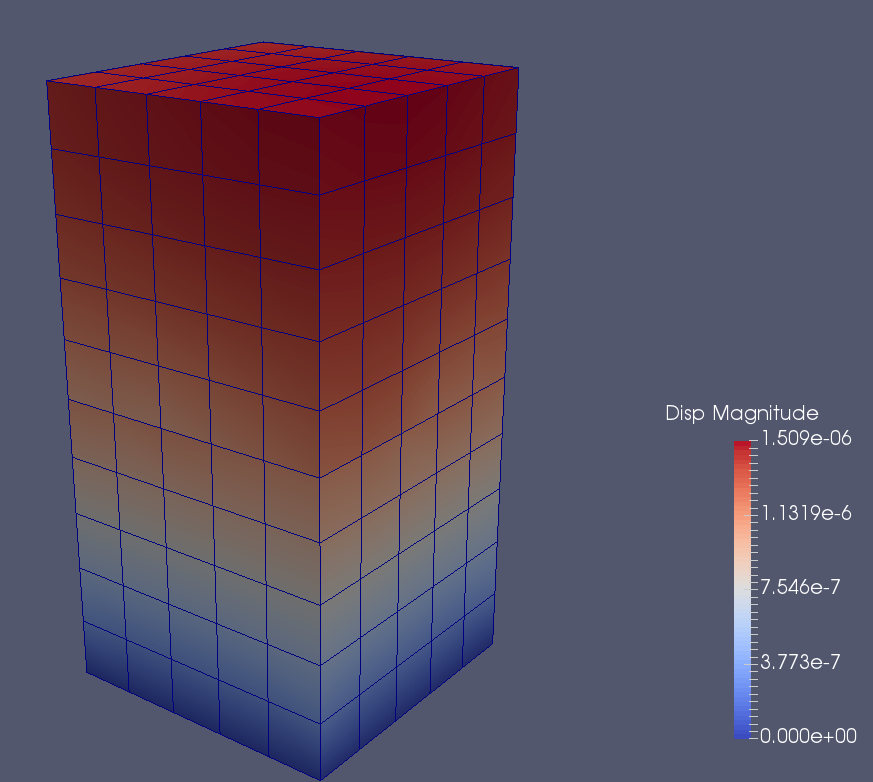
\includegraphics[height=\figillus]{../figure/Cubes_H8_5.png}$\quad$}
  \subfloat[LowWall\_FEM]{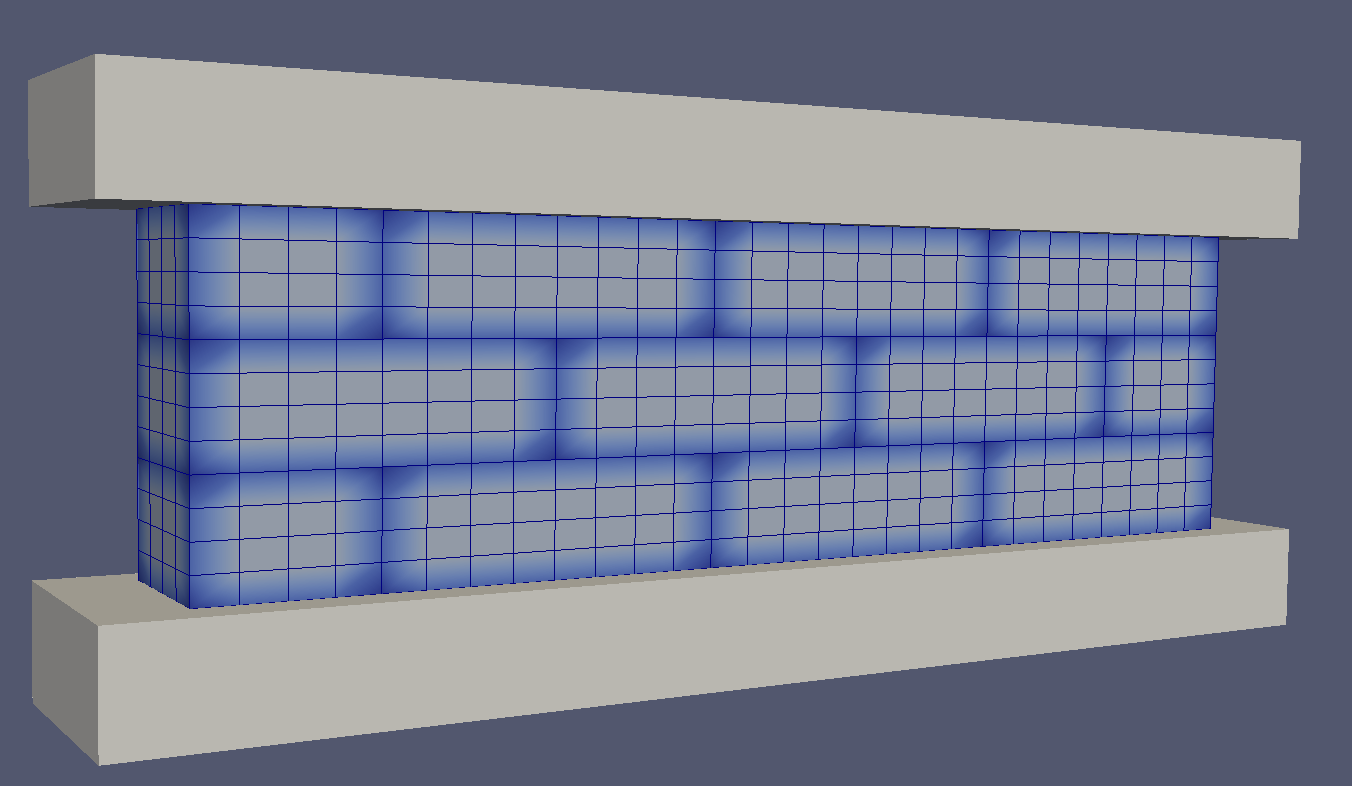
\includegraphics[height=\figillus]{../figure/LowWall_FEM.png}}\\
  \subfloat[Aqueduct\_PR]{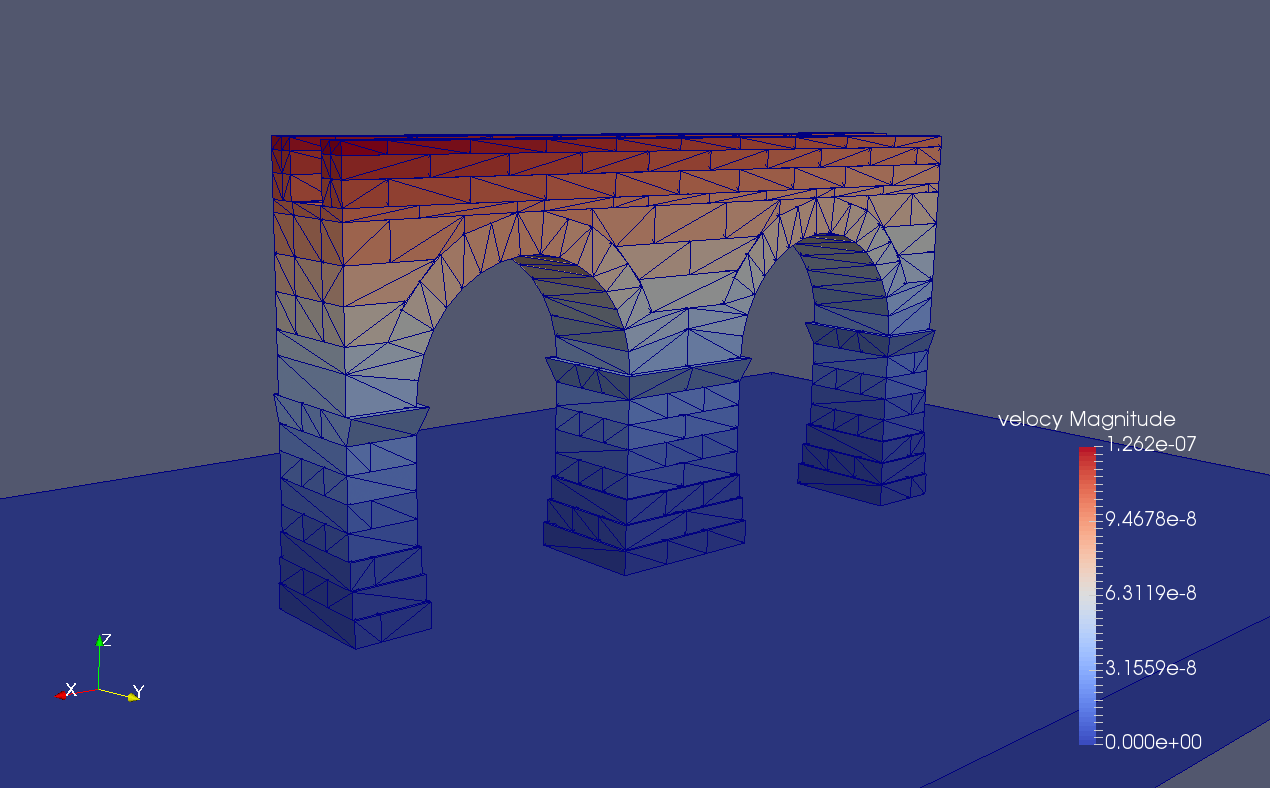
\includegraphics[height=\figillus]{../figure/Aqueduc_PR.png}$\quad$}
  \subfloat[Bridge\_PR]{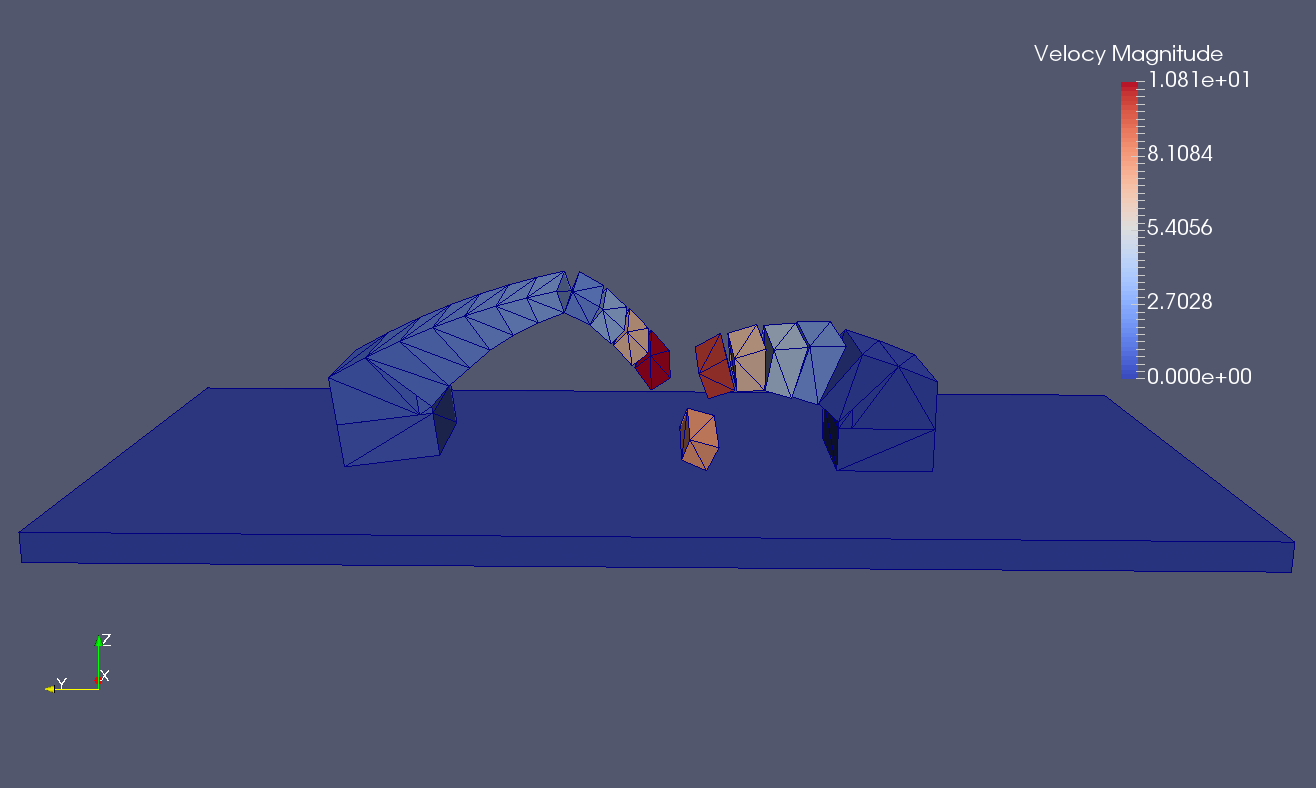
\includegraphics[height=\figillus]{../figure/Bridge_PR_1.png}}\\
  \subfloat[100\_PR\_Periobox]{\includegraphics[height=\figillus]{../figure/100_PR_Periobox.png}$\quad$}
  \subfloat[945\_SP\_Box\_PL]{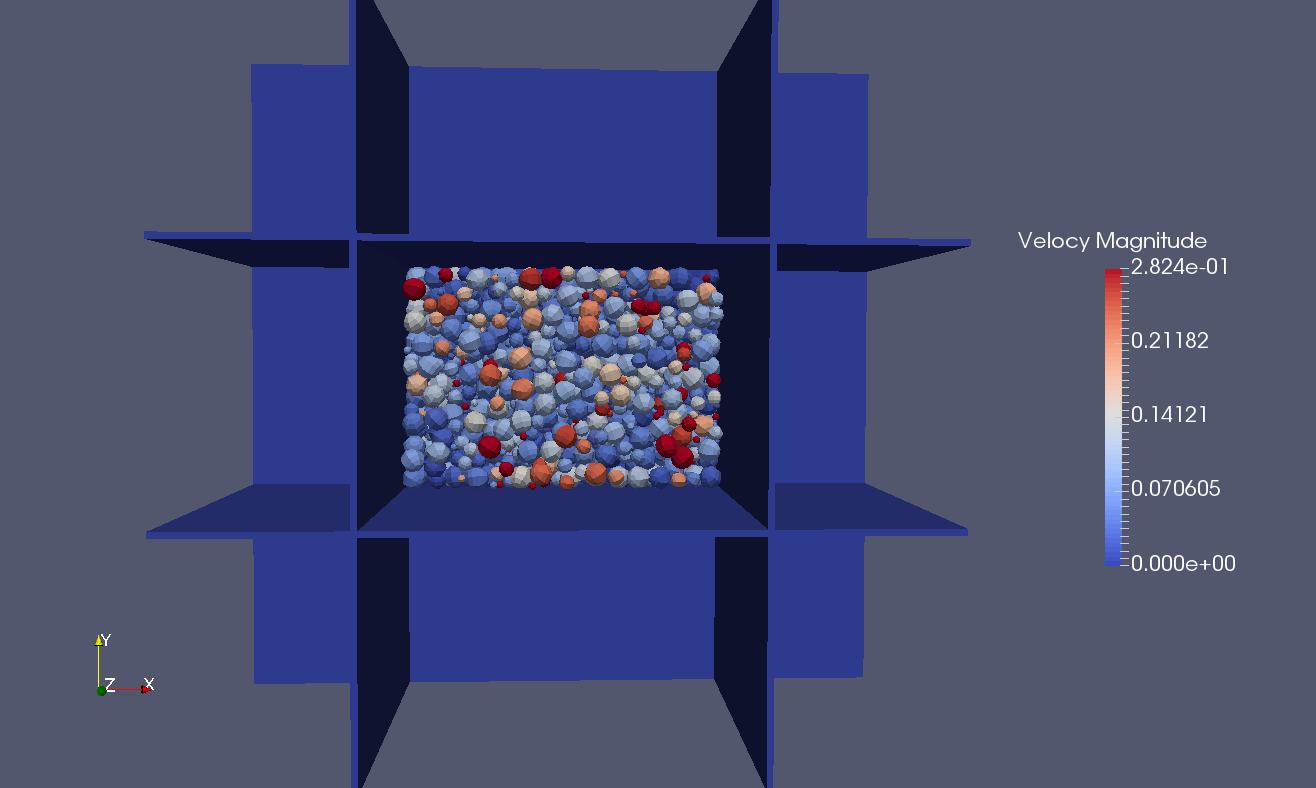
\includegraphics[height=\figillus]{../figure/945_SP_Box_PL.png}}\\
  \subfloat[Capsules]{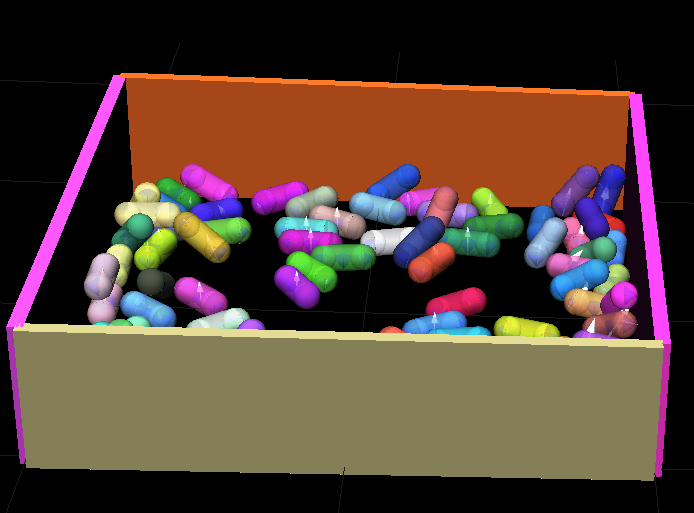
\includegraphics[height=\figillus]{../figure/Capsules.png}$\quad$}
  \subfloat[Chain]{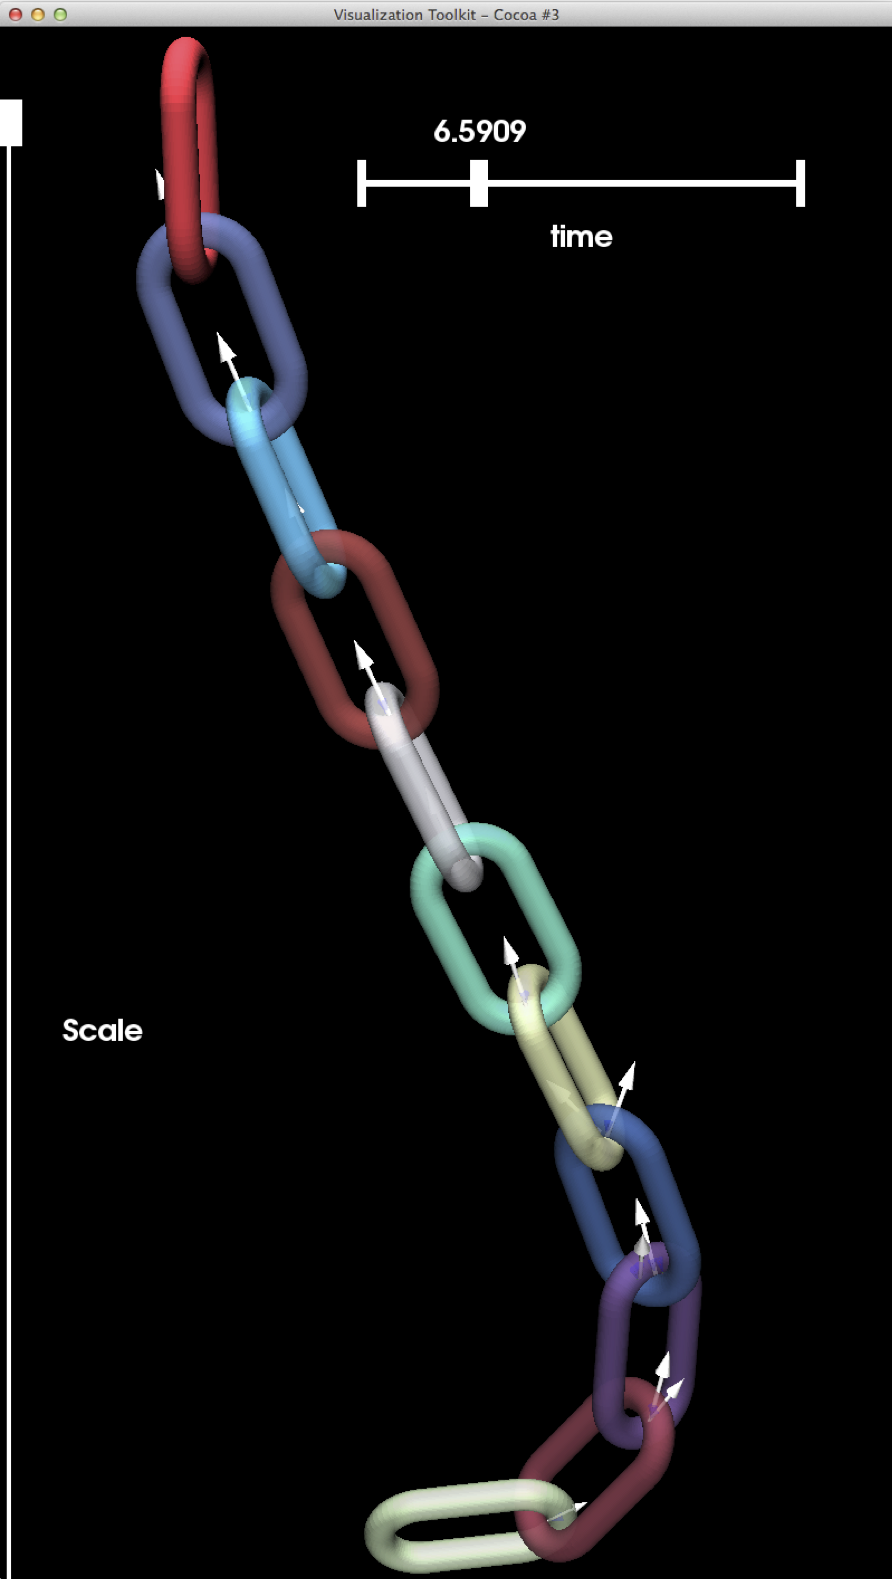
\includegraphics[height=\figillus]{../figure/Chains.png}$\quad$}
  \subfloat[KaplasTower]{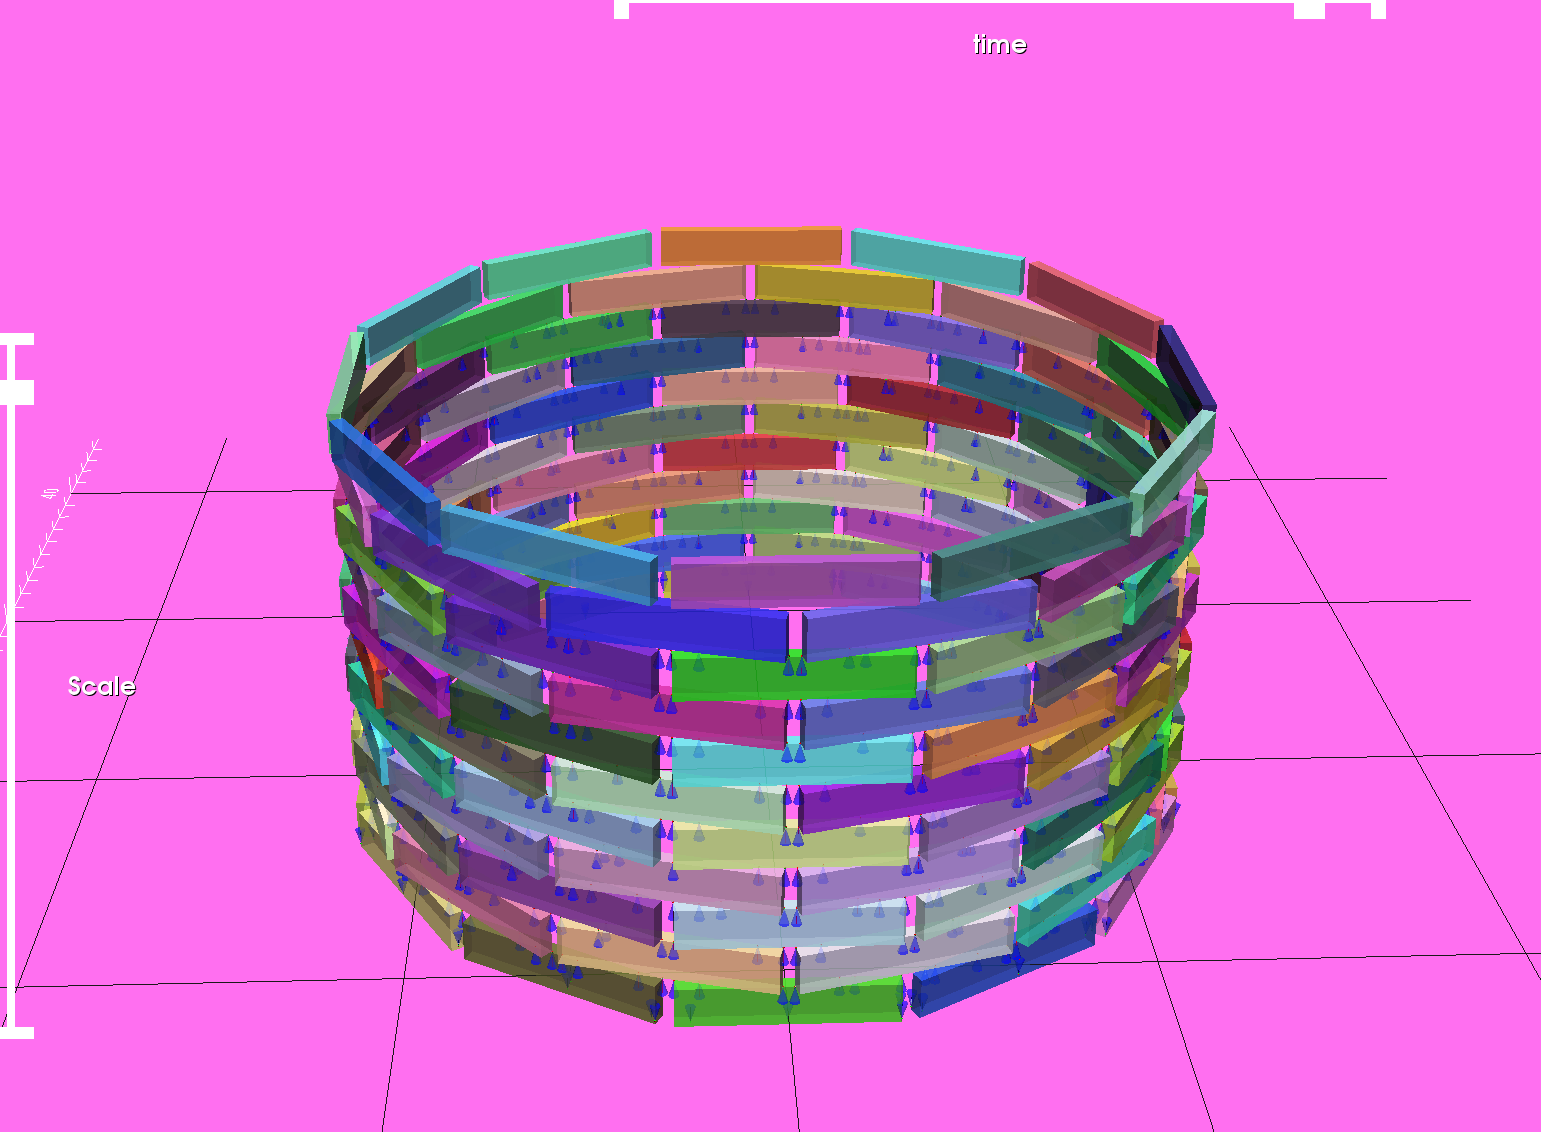
\includegraphics[height=\figillus]{../figure/KaplasTower.png}$\quad$}
  \subfloat[BoxesStack]{$\quad$$\quad$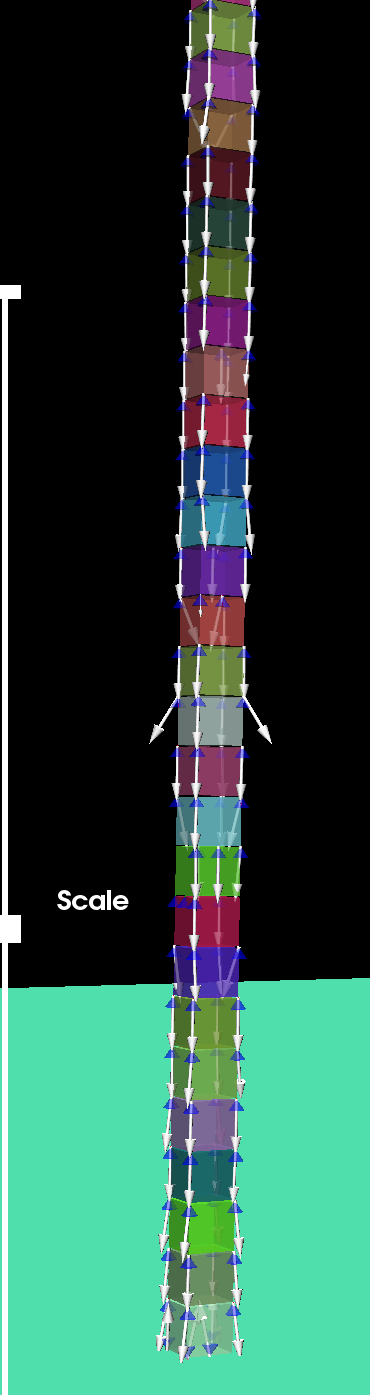
\includegraphics[height=\figillus]{../figure/BoxesStack.png}$\quad$$\quad$}\\
  \subfloat[Chute\_1000, Chute\_4000, Chute\_local\_problems]{$\quad$$\quad$$\quad$$\quad$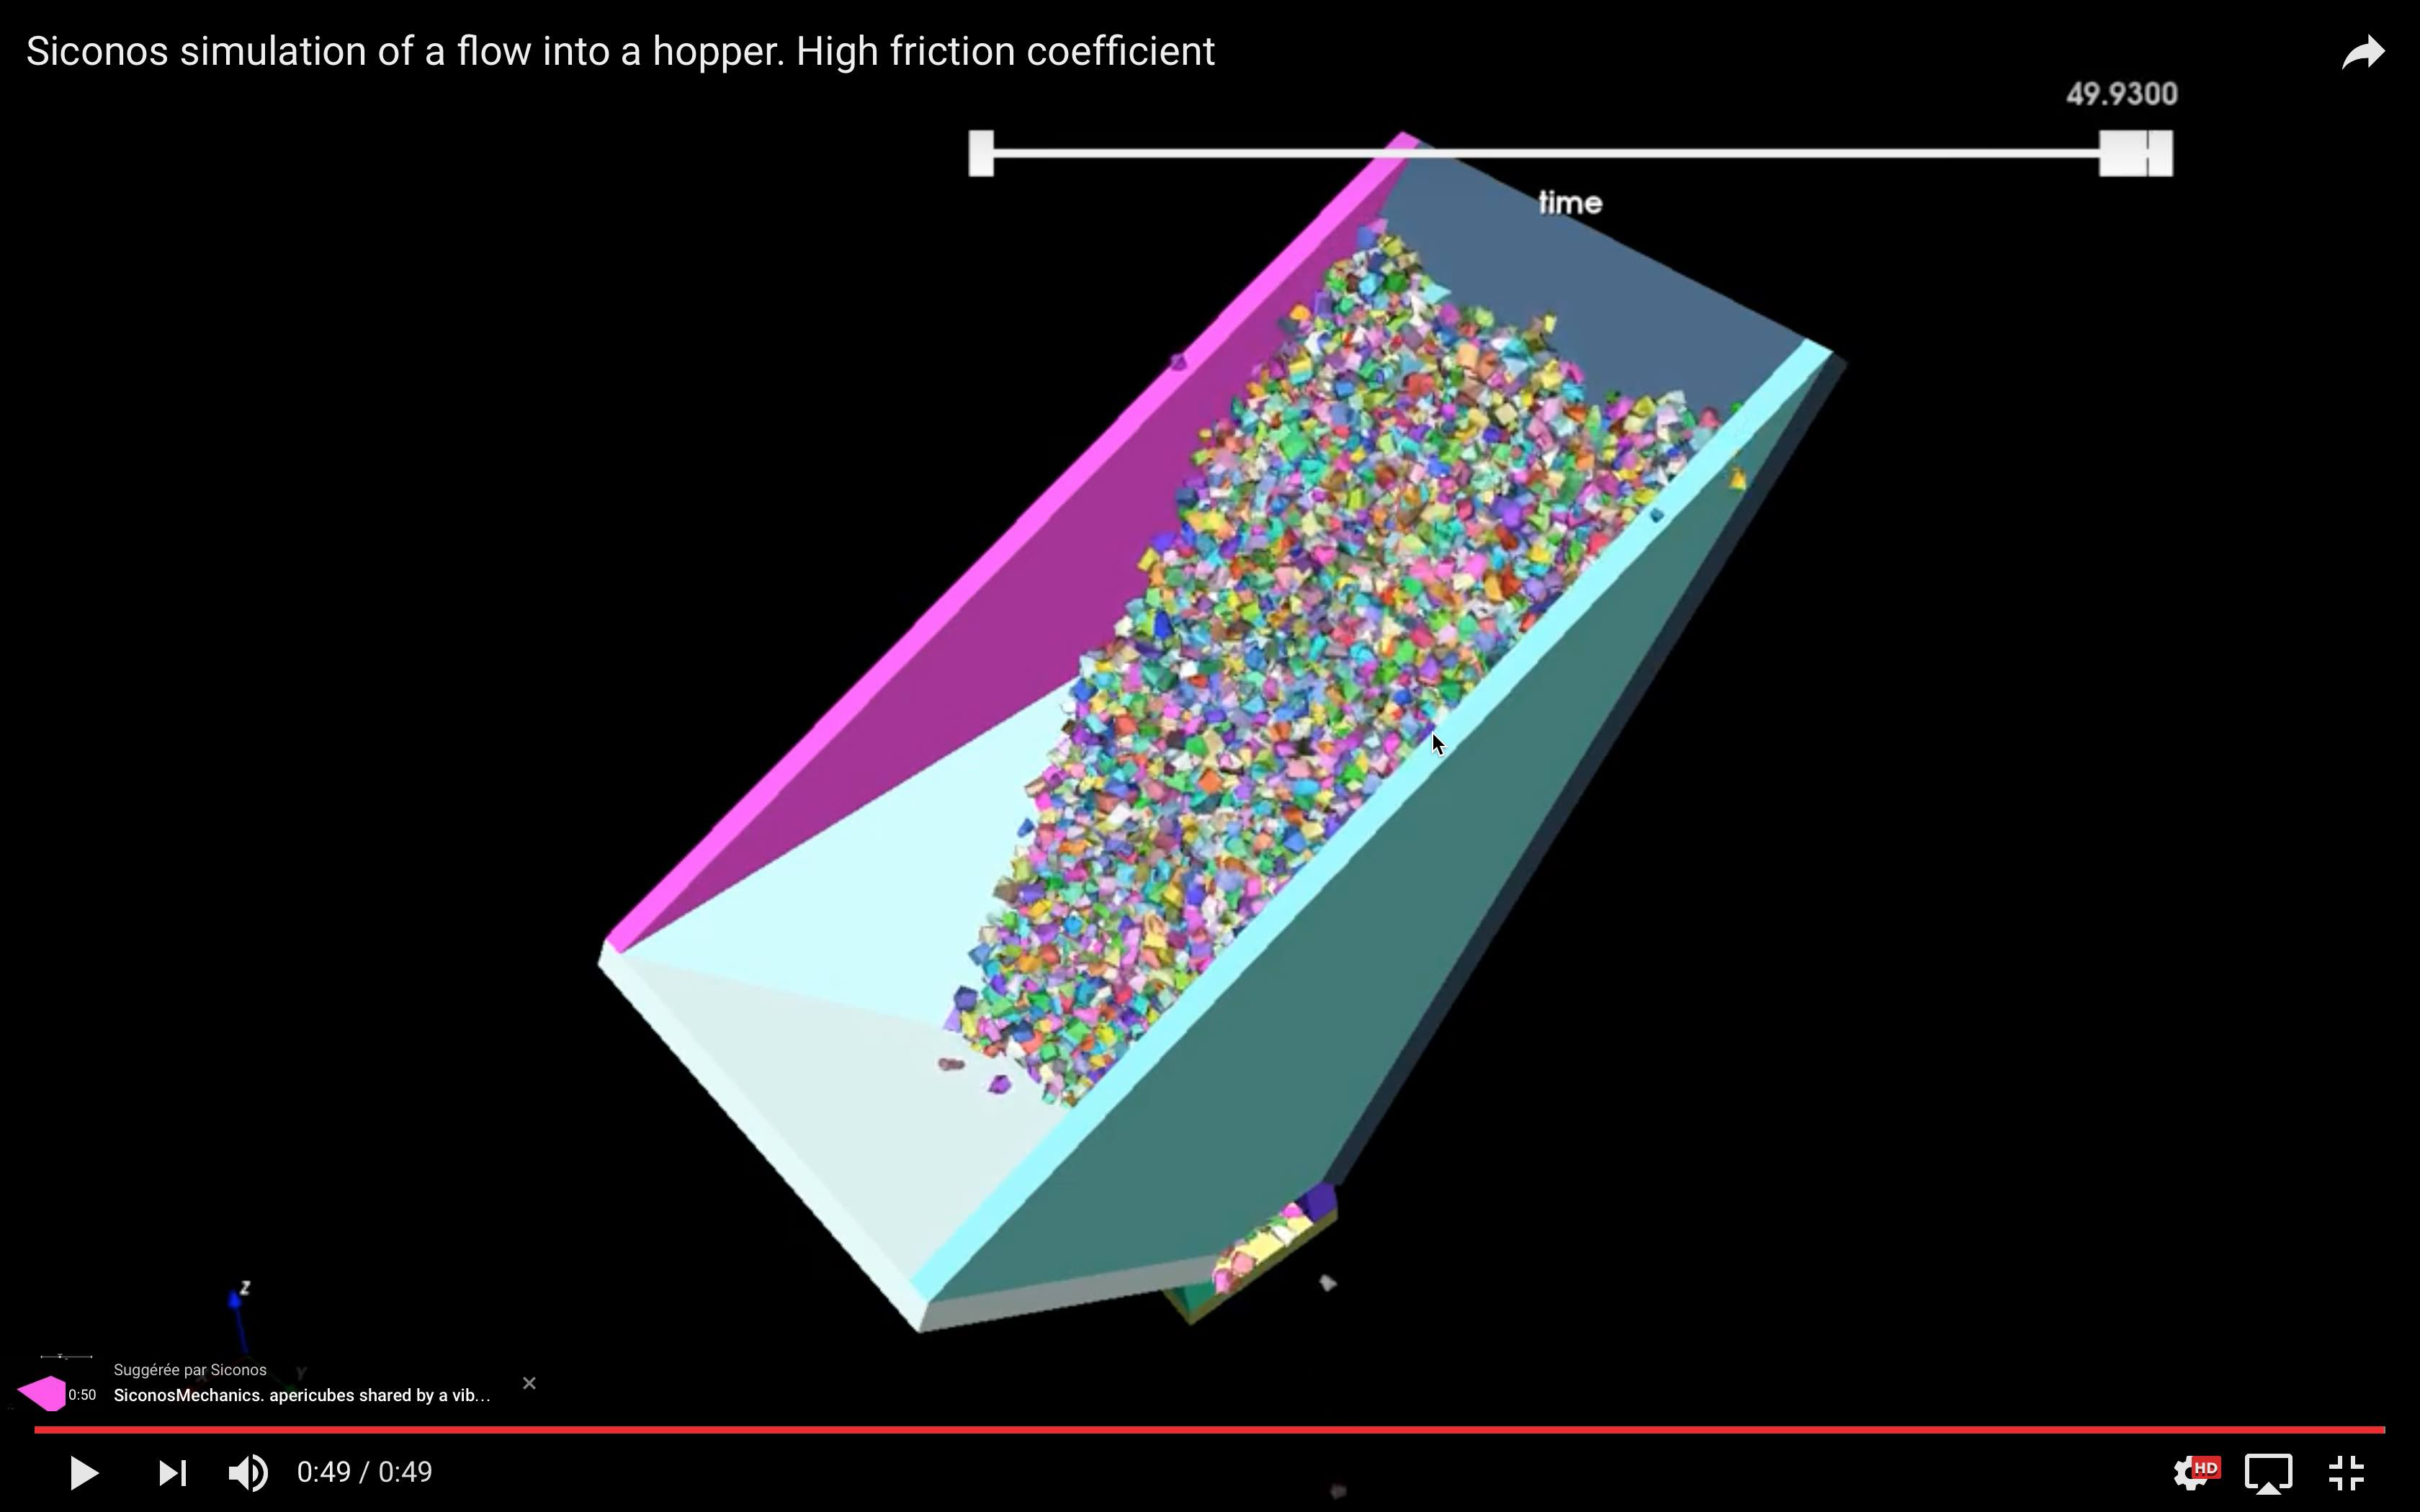
\includegraphics[height=\figillus]{../figure/Chute_1000_light.jpg}$\quad$$\quad$$\quad$$\quad$}
  \caption{Illustrations of the FClib test problems}
  \label{fig:fclib}
\end{figure}

% \begin{sidewaystable}
\begin{landscape}
  \vfill
  \begin{table}
\centering
\begin{tabular}{|l|l|l|l|l|l|l|l|l|l|l|}
  \hline
  Test set
  & code
  & \parbox[t]{2mm}{\rotatebox[origin=c]{-90}{  friction coefficient $\mu$  }}
  & \parbox[t]{2mm}{\rotatebox[origin=c]{-90}{ \# of problems }}
  & \parbox[t]{2mm}{\rotatebox[origin=c]{-90}{ \# of d.o.f. }}
  & \parbox[t]{2mm}{\rotatebox[origin=c]{-90}{ \# of contacts }}
  & \parbox[t]{2mm}{\rotatebox[origin=c]{-90}{contact density $c$}}
  %& \parbox[t]{2mm}{\rotatebox[origin=c]{-90}{rank(W)}}
  & \parbox[t]{2mm}{\rotatebox[origin=c]{-90}{rank ratio(W)}}
  & \parbox[t]{2mm}{\rotatebox[origin=c]{-90}{cond(W)}}
  & \parbox[t]{2mm}{\rotatebox[origin=c]{-90}{cond(W) LSMR}}
  \\
  \hline
  \hline
  Cubes\_H8\_2
  & LMGC90
  & 0.3
  & 15
  & 162
  & $[3:5]$
  & $[0.02:0.09]$
%  & $[6:15]$
  & 1
  & $[2.2.10^{1}:1.3.10^{3}]$
  & $[8.1.10^{5}:1.5.10^{6}]$\\
   \hline
  Cubes\_H8\_5
  & LMGC90
  & 0.3
  & 50
  & 1296
  & $[17:36]$
  & $[0.02:0.09]$
%  & $[48:108]$
  & 1
  & $[3.3.10^{4}: 7.2.10^{4} ]$
  & $[1.3.10^{6}: 3.1.10^{6} ]$\\
   \hline
  Cubes\_H8\_20
  & LMGC90
  & 0.3
  & 50
  & 55566
  & $[361:388]$
  & $[0.019:0.021]$
%  & $[1083:1164]$
  & 1
  & $[2.4.10^{5}: 2.5.10^{5} ]$
  & $[1.3.10^{6}: 5.2.10^{6} ]$\\
  \hline
  LowWall\_FEM
   & LMGC90
  & 0.83
  & 50
  & \{7212\}
  & $[624:688]$
  & $[0.28:0.29]$
%  & $[1873:2064]$
  & 1
  & --
  & $[9.3.10^{2}:5.0.10^{5}]$\\
  \hline
  Aqueduct\_PR
  & LMGC90
  & 0.8
  & 10
  & \{1932\}
  & $[4337:4811]$
  & $[6.81:7.47]$
%  & $[1934]$$
  & $[6.80:7.46]$
  & $[4.7.10^{7}:3.4.10^{8}]$
  & $[6.7.10^{1}:1.5.10^{2}]$\\
  \hline
  Bridge\_PR
  & LMGC90
  & 0.9
  & 50
  & \{138\}
  & $[70:108]$
  & $[1.5:2.3]$
%  & $[87:132]$
  & $[2.27:2.45]$
  & $[8.3.10^{4}:1.1.10^{5}]$
  & $[1.9.10^{3}:2.6.10^{4}]$\\
  \hline
  100\_PR\_Periobox
  & LMGC90
  & 0.8
  & 106
  & \{606\}
  & $[14:578]$
  & $[0.2:3]$
%  & $[23:600]$
  & $[1.76:3.215]$
  & $[4.3.10^{2}:1.0.10^{6}]$
  & $[6.3.10^{5}:3.5.10^{6}]$ \\
  \hline
  945\_SP\_Box\_PL
  & LMGC90
  & 0.8
  & 60
  & \{5700\}
  & $[2322:5037]$
  & $[1.22:2.65]$
%  & $[5333:7617]$
  & $[1.0:2.66]$
  & $[2.2.10^{4}:4.4.10^{5}]$
  & $[2.9.10^{1}:9.2.10^{2}]$\\
  \hline
  Capsules
  & Siconos
  & 0.7
  & 249
  & \{300\}
  & $[1:200]$
  & $[1.2:1.5]$
%  & $[47:587]$
  & $[1.08:1.55]$
  & $[1.2.10^{6}:7.5.10^{9}]$
  & -- \\
  \hline
  Chain
  & Siconos
  & 0.3
  & 242
  & \{60\}
  & $[8:28]$
  & $[0.5:1.3]$
%  & 53
  & $[1.05:1.6]$
  & $[7.4.10^{4}:4.0.10^{9}]$
  & $[1.5.10^{1}:4.7.10^{5}]$\\
  \hline
  KaplasTower
  & Siconos
  & 0.7
  & 201
  & $[72:792]$
  & $[48:933]$
  & $[3.0:3.6]$
%  & $[72:792]$
  & $[2.0:3.53]$
  & $[67:2174]$
  & $[8:67]$\\
  \hline
  BoxesStack
  & Siconos
  & 0.7
  & 255
  & $[6:300]$
  & $[1:200]$
  & $[1.86:2.00]$
%  & $[54:300]$
  & $[1.875:2.0]$
  & $[3.8.10^{4}:2.5.10^{7}]$
  & $[9.0:5.4.10^{3}]$\\
  \hline
  Chute\_1000
  & Siconos
  & 1.0
  & 156
  & $[276:5508]$
  & $[74:5056]$
  & $[0.69:2.95]$
%  & $[222:8133]$
  & $[1.0:2.95]$
  & $[2.1.10^{1}:1.9.10^{3}]$
  & \\
  \hline
  Chute\_4000
  & Siconos
  & 1.0
  & 40
  & $[17280:20034]$
  & $[15965:19795]$
  & $[2.51:3.06]$
  & --
  % & $[222:8133]$
  & --
  & $[5.5.10^{1}:9.0.10^{3}]$\\
  \hline
  Chute\_local\_problems
  & Siconos
  & 1.0
  & 834
  & 3
  & 1
  & 1
%  & 3
  & 1
  & $[1.04:4.66]$
  & $[2.6:2.6.10^{1}]$\\
  \hline
\end{tabular}
\caption{Description of the test sets of FCLib library (v1.0)}
\label{Tab:fclib}
\end{table}
  \vfill
\end{landscape}
%\end{sidewaystable}



\begin{ndrva}
  Can we say more on the description of the examples ?
\end{ndrva}
% \subsection{Parameters}

% \begin{itemize}
% \item size (n, m), sparsity,
% \item matrix storage
% \item conditionning $M$ $W$
% \item rank of $H$ or $W$ on active contact
% \item parameter $\nu = m_c/n$
% \end{itemize}

% \begin{itemize}
% \item algorithms parameters ($\rho$)
% \end{itemize}

\subsection{Sofware \& implementation details}

All the solvers that are used in this chapter are implemented in standard C in the component of the open source software Siconos called numerics. The aim of Siconos is to provide a common platform for the modeling, simulation, analysis and control of general nonsmooth dynamical systems\footnote{More information on the software is available at \href{http://siconos.gforge.inria.fr}{http://siconos.gforge.inria.fr} and the software can be downloaded at  \href{https://github.com/siconos/siconos}{https://github.com/siconos/siconos}}. The algebraic manipulations are based on BLAS/LAPACK. The algorithms {\sf VI-FP}, {\sf VI-EG}, {\sf NSGS} and {\sf PSOR} use the sparse block structure of the Delassus matrix $W$ and we solve . The {\sf NSN} solvers relies on a standard sparse implementation given by csparse\footnote{\href{http://people.sc.fsu.edu/~jburkardt/c_src/csparse/csparse.html}{http://people.sc.fsu.edu/~jburkardt/c\_src/csparse/csparse.html}} and we use the linear solver based on LU factorization embedded in csparse. The simulations are performed on the University of Grenoble-Alpes cluster {\sc ciment}\footnote{https://ciment-grid.ujf-grenoble.fr/}.





\begin{ndrva}
 something more ?
\end{ndrva}

\subsection{Simulation campaign}
The simulation campaign is described in Table~\ref{Tab:fclib-simulation}. For some test sets, two simulations runs have been performed with different precisions and prescribed time limits. A trade-off between the time limit and the precision has been chosen such that all the problems of the test sets are solved at least by one solver within the prescribed time limit.


\begin{table}
\centering
\begin{tabular}{|l|l|l|l|l|l|l|l|}
  \hline
  Test set
  & \parbox[t]{3mm}{\rotatebox[origin=c]{90}{ precision }}
  & \parbox[t]{3mm}{\rotatebox[origin=c]{90}{ prescribed time limit (s) }}
  & \parbox[t]{3mm}{\rotatebox[origin=c]{90}{ mean performance  }}
    \parbox[t]{3mm}{\rotatebox[origin=c]{90}{ of the fastest solver }}
    \parbox[t]{3mm}{\rotatebox[origin=c]{90}{$\mu\{\min\{t_{p,s}, s\in S\}\}$  }}
  &  \parbox[t]{3mm}{\rotatebox[origin=c]{90}{ std. deviation performance  }}
    \parbox[t]{3mm}{\rotatebox[origin=c]{90}{ of the fastest solver }}
    \parbox[t]{2mm}{\rotatebox[origin=c]{90}{ $\sigma({\min\{t_{p,s}, s\in S\}})$  }}
  & \parbox[t]{3mm}{\rotatebox[origin=c]{90}{ mean performance  }}
    \parbox[t]{3mm}{\rotatebox[origin=c]{90}{ of the fastest solver by contact }}
    \parbox[t]{3mm}{\rotatebox[origin=c]{90}{$\mu\{\min\{t_{p,s}/n_{c,p}, s\in S\}\}$  }}
  &  \parbox[t]{3mm}{\rotatebox[origin=c]{90}{ std. deviation performance  }}
    \parbox[t]{3mm}{\rotatebox[origin=c]{90}{ of the fastest solver by contact  }}
    \parbox[t]{2mm}{\rotatebox[origin=c]{90}{ $\sigma({\min\{t_{p,s}/n_{c,p}, s\in S\}})$  }}
  & \parbox[t]{3mm}{\rotatebox[origin=c]{90}{ \# of unsolved problems  }}
  \\
  \hline
  \hline
  Cubes\_H8\_$\star$
  & $10^{-08}$
  & 100
  & 1.73
  & 2.13
  & $4.83^{-03}$
  & $5.78^{-03}$
  & 0\\
  \hline
  Cubes\_H8\_$\star$ II
  & $10^{-04}$
  & 100
  & 0.92
  & 1.06
  & $2.66^{-03}$
  & $2.83^{-03}$
  & 0\\
  \hline
  LowWall\_FEM
  & $10^{-04}$
  & 400
  & 14.8
  & 2.85
  & $2.16^{-02}$
  & $4.54^{-03}$
  & 0
    \\
  \hline
  Aqueduct\_PR
  & $10^{-04}$
  & 200
  & 5.80
  & 6.36
  & $4.90^{-04}$
  & $3.03^{-04}$
  & 0
  \\
  \hline
  Bridge\_PR
  & $10^{-08}$
  & 400
  & 10.3
  & 12.9
  & $1.23^{-01}$
  & $2.88^{-01}$
  & 0\\
  \hline
  Bridge\_PR II
  & $10^{-04}$
  & 100
  & 0.048
  & 0.038
  & $1.30^{-03}$
  & $1.42^{-03}$
  & 0\\
  \hline
  100\_PR\_Periobox
  & $10^{-04}$
  & 100
  & 0.064
  & 0.062
  & $1.56^{-04}$
  & $1.22^{-04}$
  & 0
  \\
  \hline
  945\_SP\_Box\_PL
  & $10^{-04}$
  & 100
  & 3.20
  & 1.71
  & $6.45^{-04}$
  & $3.36^{-04}$
  & 0
  \\
  \hline
  Capsules
  & $10^{-08}$
  & 50
  & $1.46.10^{-02}$
  & $1.74.10^{-02}$
  & $5.67^{-05}$
  & $6.26^{-05}$
  & 0
  \\
  \hline
  Chain
  & $10^{-08}$
  & 50
  & $6.19.10^{-04}$
  & $3.68.10^{-04}$
  & $3.15.10^{-05}$
  & $1.46.10^{-05}$
  & 0
  \\
  \hline
  KaplasTower
  & $10^{-08}$
  & 200
  & $1.27.10^{-01}$
  & $3.75.10^{-01}$
  & $1.84.10^{-04}$
  & $4.57.10^{-04}$
  & 0
  \\
  \hline
  KaplasTower II
  & $10^{-04}$
  & 100
  & $2.84.10^{-02}$
  & $1.51.10^{-01}$
  & $3.39.10^{-05}$
  & $1.84.10^{-04}$
  & 0
  \\
  \hline
  BoxesStack
  & $10^{-08}$
  & 100
  & $3.42.10^{-02}$
  & $8.87.10^{-02}$
  & $3.24.10^{-04}$
  & $9.77.10^{-04}$
  & 0
  \\
  \hline
  Chute\_1000
  & $10^{-04}$
  & 200
  & 2.62
  & 3.06
  & $6.76^{-04}$
  & $6.58^{-04}$
  & 0
  \\
  \hline
  Chute\_4000
  & $10^{-04}$
  & 200
  & 10.52
  & 7.88
  & $5.71^{-04}$
  & $4.07^{-04}$
  & 0
  \\
  \hline
  Chute\_local\_problems
  & $10^{-08}$
  & 10
  & $1.80.10^{-04}$
  & $1.57.10^{-05}$
  & $1.80.10^{-04}$
  & $1.57.10^{-05}$
  &  0 \\
  \hline
  % Chute\_local\_problems II
  % & $10^{-04}$
  % & 10
  % & $2.00.10^{-04}$
  % & $1.91.10^{-05}$
  % & $2.00.10^{-04}$
  % & $1.91.10^{-05}$
  % &  0 \\
  % \hline
\end{tabular}
\caption{Parameters of the simulation campaign}
\label{Tab:fclib-simulation}
\end{table}

In Sections~\ref{Sec:ComparisonFamily} and~\ref{Sec:Comparison}, we report the results for the simulation campaign. The simulations campaign represents more that $27000$ runs to complete all the simulations of all problems with all the variants of the solvers.  Since the large amount of data and the numerous of performance profiles for each test sets that are generated, we do not report any profiles  when a list of solvers fails or is not able to meet the required tolerance within the prescribed time defined by the timeout values\footnote{Nevertheless, the reader can have access to the complete list of performance profiles at \href{https://github.com/siconos/faf/blob/master/TeX/Full-test/full-test_current.pdf}{https://github.com/siconos/faf/blob/master/TeX/Full-test/full-test\_current.pdf}}.


\begin{ndrva}
 a permanent address on hal  would be better
\end{ndrva}




%\newcommand\commentedfigure[1]{#1}
\newcommand\commentedfigure[1]{}


\makeatletter
\def\subfigcounter{\thesubfigure}
%\def\subfigcounter{\thefigure}
\makeatother



\def\subfiglayout{%
  \captionsetup[subfloat]{farskip=-0pt,captionskip=-2pt,font=scriptsize}%
  \setlength{\abovecaptionskip}{0pt}}
%\def\subfiglayout{}
\def\measurename{time}
\def\performance{time}
\def\widthfigure{0.6}
\def\figwidth{0.50\textwidth}
\def\legendwidth{0.6\textwidth}
\def\legendheight{0.15\textheight}

\section{Comparison of methods by family}
\label{Sec:ComparisonFamily}
In this section, we perform a comparison of the solvers by family by family. The goal is  to study the influence of the various parameters and possible strategies on the performance of the solvers.

\subsection{Numerical methods for VI: {\sf FP-DS, FP-VI-$\star$} and {\sf FP-EG-$\star$}}
\label{Sec:Comparison,VI,step-length}


In Figure~\ref{fig:VI/UpdateRule}, we compare the different numerical solvers for VI described in Section~\ref{sec:numericalmethods,vi}. The solvers are quite slow to converge in practice for large problems and/or with tight tolerances although they are robust except for {\sf FP-DS}. Only the test sets for which the solvers are reached the precision before the prescribed time limit are presented. For that reason, the results for the test sets LowWall\_FEM,  Cubes\_H8, Bridge\_PR, AqueducPR, 945\_SP\_Box\_PL, BoxesStack, Chute\_4000  and Chute\_1000  are not depicted. 
The main conclusions are as follows:
\begin{enumerate}
\item The solver {\sf FP-DS} suffers from robustness problems and a lot of divergence has been observed. This is mainly due to the fact that we set a priori the $\rho$ parameter in Algorithm~\ref{Algo:FP-vi} to a fixed value of $1$, independently of the problem.
\item The solvers {\sf FP-VI-$\star$} and {\sf FP-EG-$\star$} are really robust but slow. They are able to solve all the problems but they require a lot of time. We did not observe divergence issues on all the test sets for these solvers. Comparing to {\sf FP-DS}, the self-adaptive rule for sizing the paramater $\rho_k$ is of utmost importance for the  robustness and the convergence rate.
\item Except for the test set KaplasTower II, the  {\sf FP-EG-$\star$} performs better than  {\sf FP-VI-$\star$}.
\item The difference between the adaptive strategy for sizing $\rho_k$, {\sf UPK} and {\sf UPTS}, is negligible in all the test sets. Therefore, the choice of the update rule is not really important.
\end{enumerate}
\begin{figure*}[htbp]
  \centering
  \subfiglayout
%\subfloat[\scriptsize LowWall\_FEM]
%  {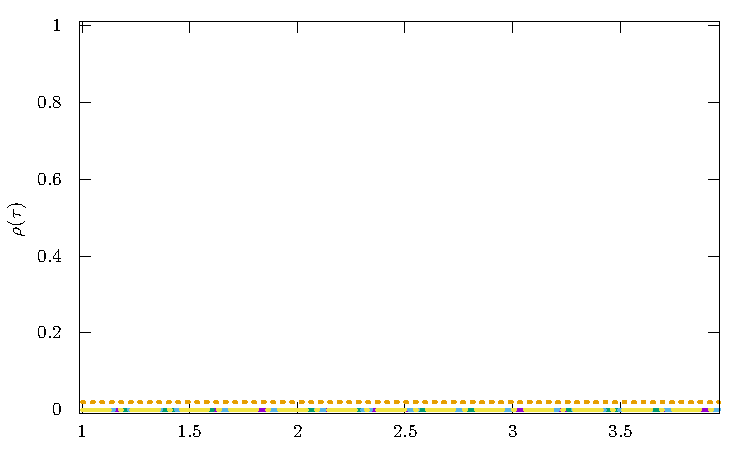
\includegraphics[width=\figwidth]{../figure/VI/UpdateRule/1.0e-04/400/time/profile-LMGC_LowWall_FEM.pdf}} %
\subfloat[ Cubes\_H8 II]
 {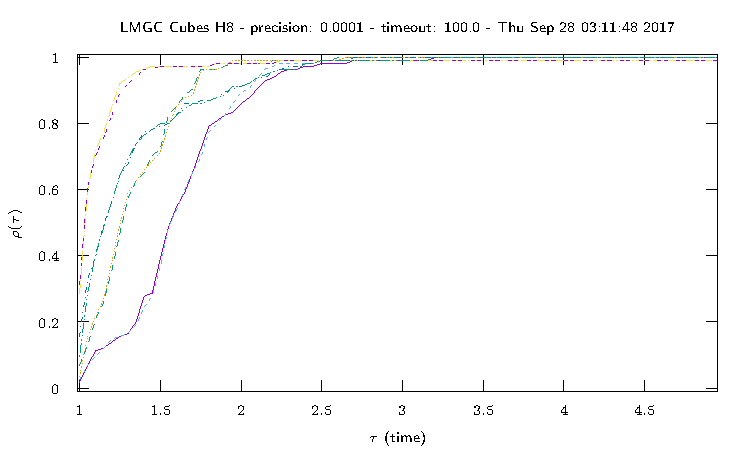
\includegraphics[width=\figwidth]{../figure/VI/UpdateRule/1.0e-04/100/time/profile-LMGC_Cubes_H8.pdf}} 
 % \subfloat[\scriptsize Cubes\_H8]
   % {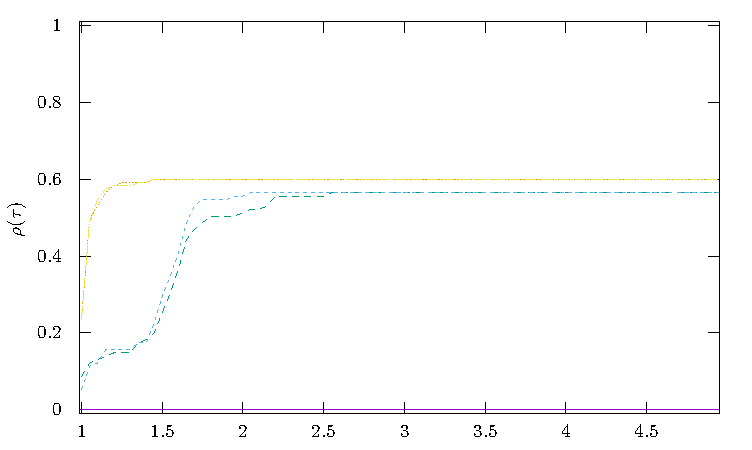
\includegraphics[width=\figwidth]{../figure/VI/UpdateRule/1.0e-08/100/time/profile-LMGC_Cubes_H8.pdf}} 
 \subfloat[\scriptsize Bridge\_PR II]
 {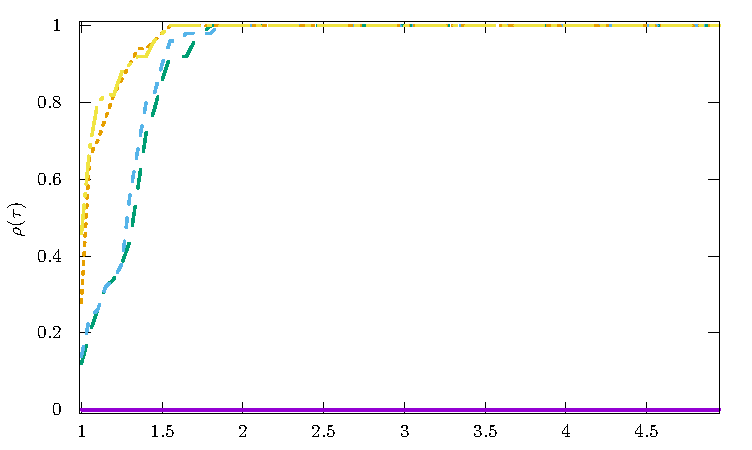
\includegraphics[width=\figwidth]{../figure/VI/UpdateRule/1.0e-04/100/time/profile-LMGC_Bridge_PR.pdf}}\\
% \subfloat[\scriptsize Bridge\_PR]
%    {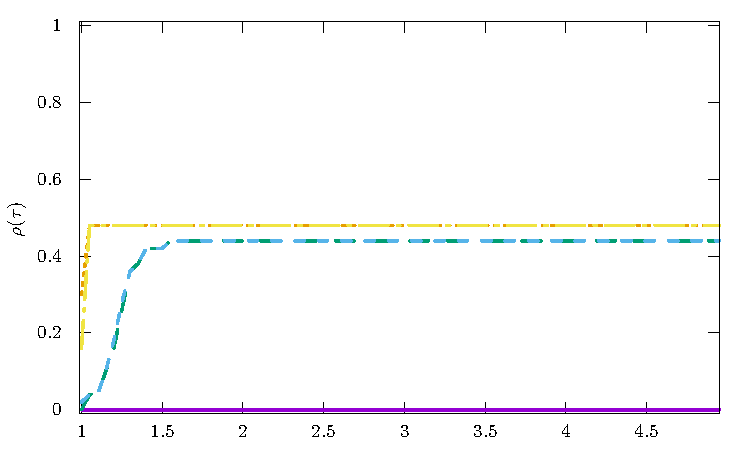
\includegraphics[width=\figwidth]{../figure/VI/UpdateRule/1.0e-08/400/time/profile-LMGC_Bridge_PR.pdf}} 
% \subfloat[\scriptsize AqueducPR]
%    {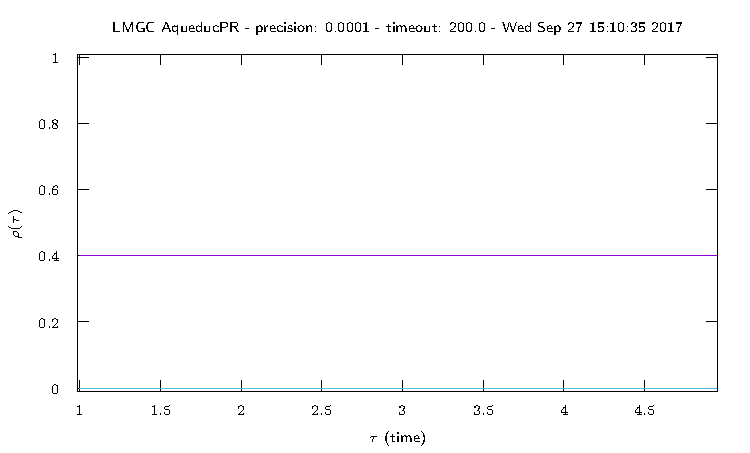
\includegraphics[width=\figwidth]{../figure/VI/UpdateRule/1.0e-04/200/time/profile-LMGC_AqueducPR.pdf}} 
% \subfloat[\scriptsize 945\_SP\_Box\_PL]
%    {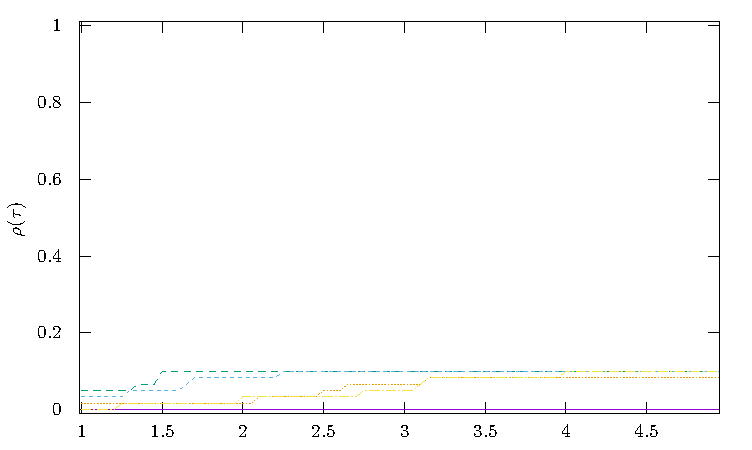
\includegraphics[width=\figwidth]{../figure/VI/UpdateRule/1.0e-04/100/time/profile-LMGC_945_SP_Box_PL.pdf}} 
 \subfloat[\scriptsize 100\_PR\_PerioBox]
{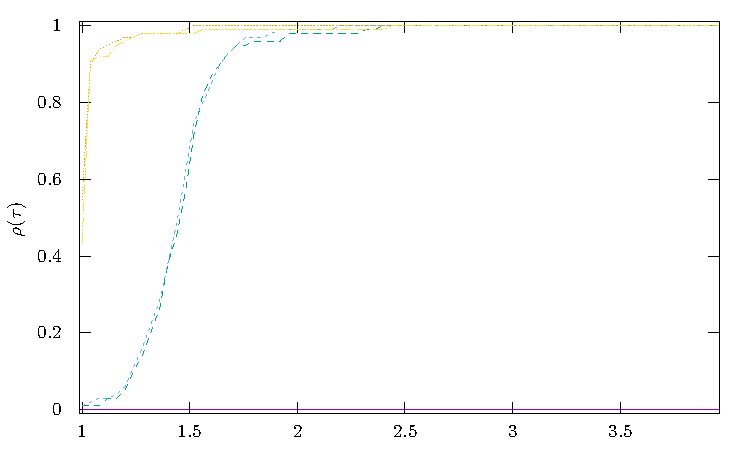
\includegraphics[width=\figwidth]{../figure/VI/UpdateRule/1.0e-04/100/time/profile-LMGC_100_PR_PerioBox.pdf}}
\subfloat[\scriptsize KaplasTower II]
   {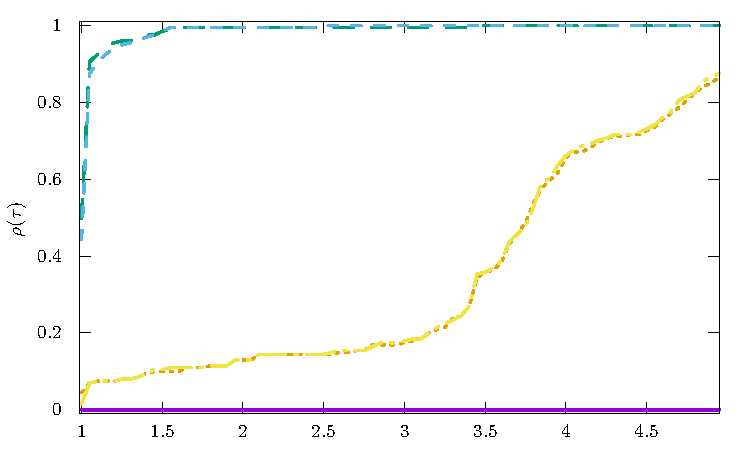
\includegraphics[width=\figwidth]{../figure/VI/UpdateRule/1.0e-04/100/time/profile-KaplasTower.pdf}} \\
\subfloat[\scriptsize KaplasTower]
   {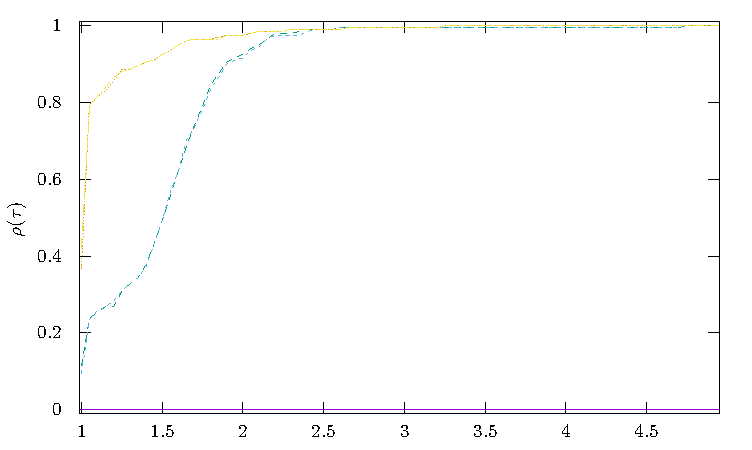
\includegraphics[width=\figwidth]{../figure/VI/UpdateRule/1.0e-08/200/time/profile-KaplasTower.pdf}} 
% \subfloat[\scriptsize Chute\_local\_problems]
%    {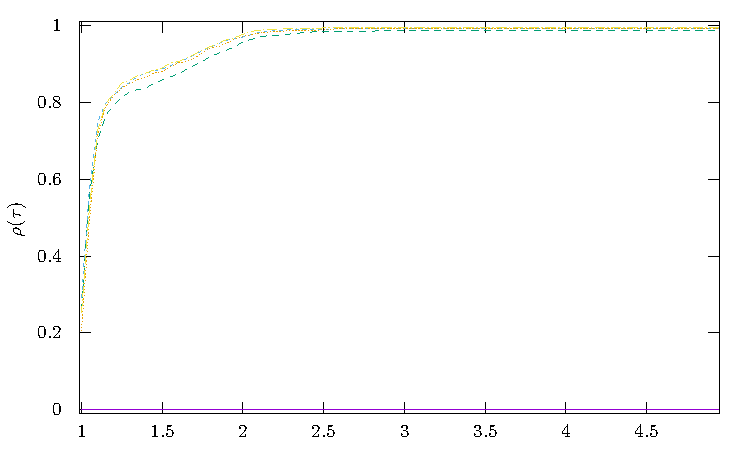
\includegraphics[width=\figwidth]{../figure/VI/UpdateRule/1.0e-08/10/time/profile-Chute_local_problems.pdf}} 
% \subfloat[\scriptsize Chute\_4000]
%    {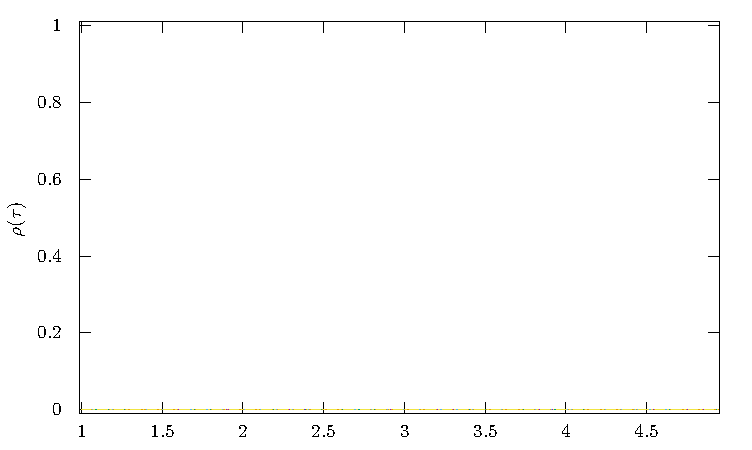
\includegraphics[width=\figwidth]{../figure/VI/UpdateRule/1.0e-04/200/time/profile-Chute_4000.pdf}} 
% \subfloat[\scriptsize Chute\_1000]
%    {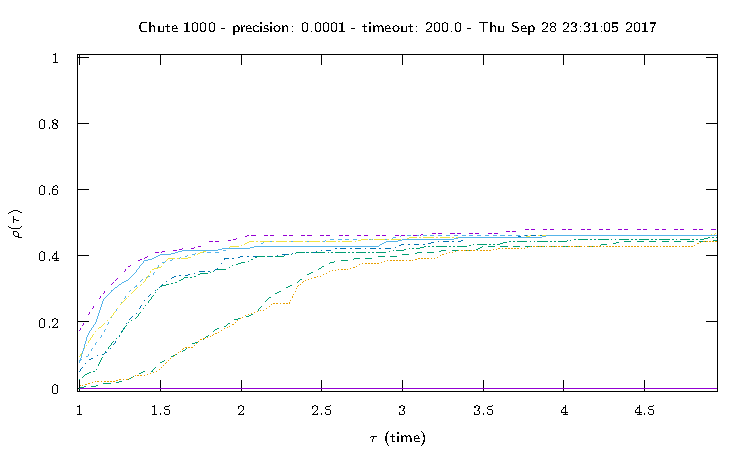
\includegraphics[width=\figwidth]{../figure/VI/UpdateRule/1.0e-04/200/time/profile-Chute_1000.pdf}} \\
% \subfloat[\scriptsize Chain]
%    {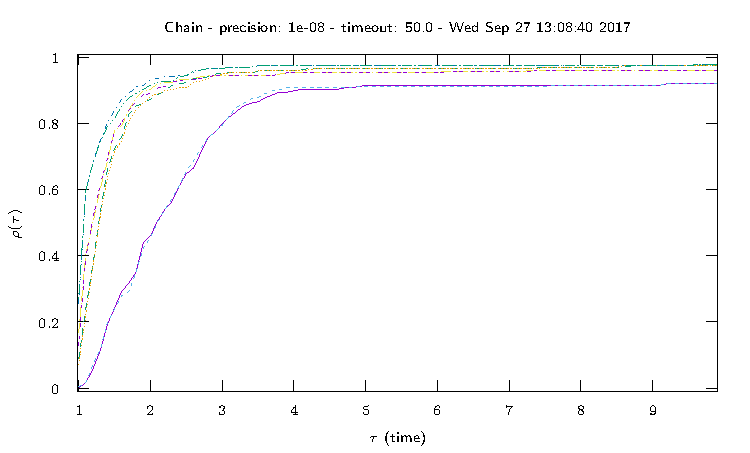
\includegraphics[width=\figwidth]{../figure/VI/UpdateRule/1.0e-08/50/time/profile-Chain.pdf}} 
\subfloat[\scriptsize Capsules]
   {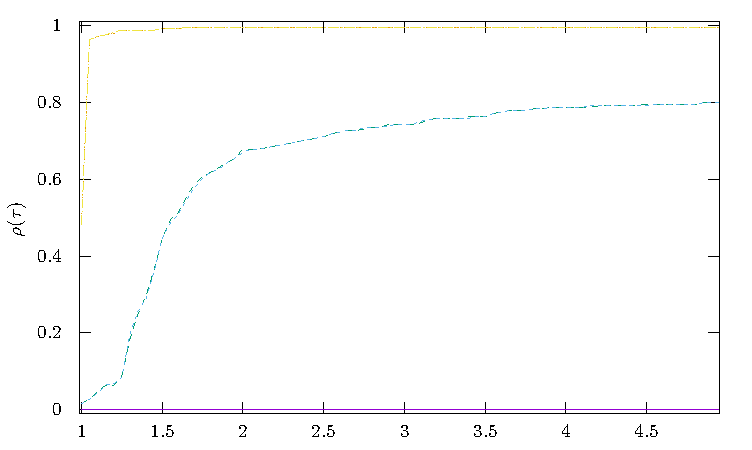
\includegraphics[width=\figwidth]{../figure/VI/UpdateRule/1.0e-08/50/time/profile-Capsules.pdf}} \\
% \subfloat[\scriptsize BoxesStack]
%    {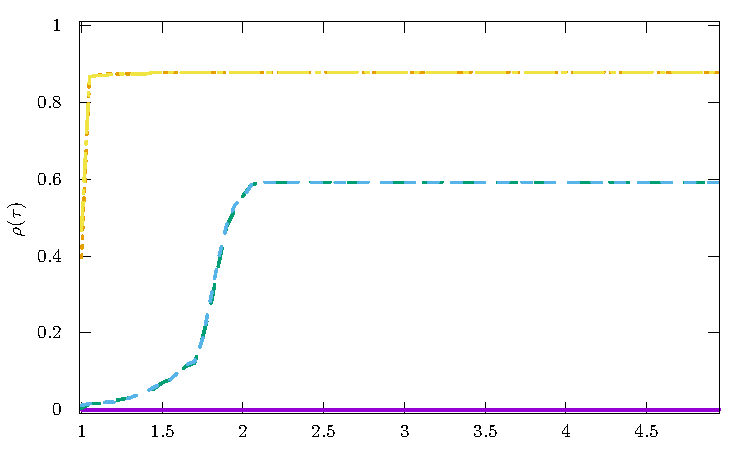
\includegraphics[width=\figwidth]{../figure/VI/UpdateRule/1.0e-08/100/time/profile-BoxesStack1.pdf}} \\
   {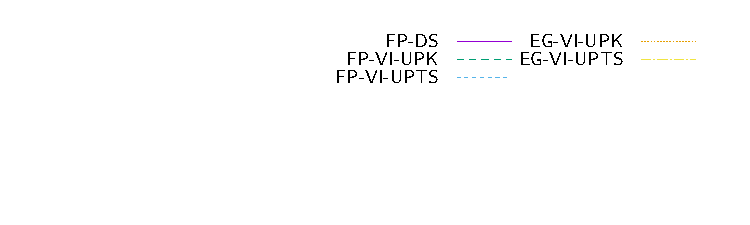
\includegraphics[height=\legendheight]{../figure/VI/UpdateRule/1.0e-08/50/time/profile-Chain_legend.pdf}}
   \setlength{\abovecaptionskip}{-40pt}
   \caption{Comparison of numerical methods {\sf FP-DS, FP-VI-$\star$} and {\sf FP-EG-$\star$}}
\label{fig:VI/UpdateRule}
\end{figure*}



\subsection{Splitting based algorithms: {\sf NSGS-$\star$} and {\sf PSOR-$\star$}}

In this section, we compare the family of solvers based on splitting and relaxation techniques described in Section~\ref{Sec:SplittingTechniques}. Firstly, we start by comparing the choice of the local solvers in {\sf NSGS-$\star$} and then the effect of the local tolerance $\sf tol_{local}$. Secondly, we study the influence of the order  of the contact list. Finally, we study the effect of the relaxation parameter $\omega$ in  {\sf PSOR-$\star$} solvers. 

\paragraph{Influence of the local solver in {\sf NSGS-$\star$}  algorithms} In Figure~\ref{fig:NSGS/LocalSolver}, we report the performance profiles of the  {\sf NSGS-$\star$} for the different local solvers.  The main conclusions are:
\begin{enumerate}
\item When the prescribed time limit is sufficiently large and the tolerance is low ($10^{-4}$), we observe the {\sf NSGS-$\star$} solvers are robust. Indeed, we are able to find to a local solver for each test sets that is able to give a solution at the required low accuracy. Nevertheless, there is no universal efficient local solver that outperforms the other ones.
  
\item When the tolerance is equal to $10^{-8}$,  the {\sf NSGS-$\star$} solvers have some difficulties to reach convergence for all the problems within the prescribed time limit. This is the case for the test sets Cubes\_H8, Bridge\_PR, Chain,  Capsules and BoxesStack. Generally, the convergence is so slow that it is difficult to reach tight tolerance with a reasonable time limit.
 
\item Except for the test sets KaplasTower II and BoxesStack, the solver {\sf NSGS-EXACT} behaves poorly. This is mainly due to the fact that the solver is not robust to find a solution for one contact when we are far from the global solution for all the contacts. This behavior was already reported in~\citep{Daviet.ea_SIGGRAPH2011} where another solver based a nonsmooth Newton technique is used when  the exact solution is not satisfactory.
  
\item  The {\sf NSGS-FP-DS-One} solver  is most efficient on the test sets Bridge\_PR II, KaplasTower II, Chain and BoxesStack. In these tests sets, a part of problems seem easier to solve and the {\sf NSGS-FP-DS-One} solver seems sufficient to get a global convergence.
  Nevertheless, this local solver seems slow or suffers from robustness issues for other test sets.
  
\item On the flexible test sets and 945\_SP\_Box\_PL, Chute\_4000, the best solver is {\sf NSGS-FP-VI-UPK} for a relatively low required tolerance ($\sf tol_{local} =10^{-06}$). For these test sets, an approximate solution of the single contact problems seems sufficient to ensure an efficient convergence towards the solution without entailing robustness.
  
\item On the test sets 100\_PR\_PerioBox, KaplasTower,  Chain, Capsules, the solver {\sf NSGS-NSN-$\star$} are the best solvers and behave very well on Bridge\_PR II. It seems that when a tight accuracy is required, the solvers {\sf NSGS-NSN-$\star$} are useful and helps with a tight local tolerance to speed-up the convergence.
  
\item For the Chute\_1000, Chute\_4000 test sets, we observe large differences between the local formulations of the nonsmooth equations for the Newton solvers ({\sf NSGS-NSN-AC} or {\sf NSGS-NSN-JM}). The solver {\sf NSGS-NSN-JM} is the best solver and really better than {\sf NSGS-NSN-AC} although their theoretical formulation are very close. Theses two test sets are characterized by difficult local problems where the Delassus matrix  $W$ is unsymmetric with large extra-diagonal terms.
\item For almost the tests, the line--search procedures slow down the solvers without increasing the robustness. The only test sets where is has interest is Chute\_4000 where the {\sf NSGS-AC} solver fails to get a solution and the line--search seems to stabilize the algorithm.
\end{enumerate}
  \begin{figure}
    \centering
    \subfiglayout
    \subfloat[\scriptsize LowWall\_FEM]
    {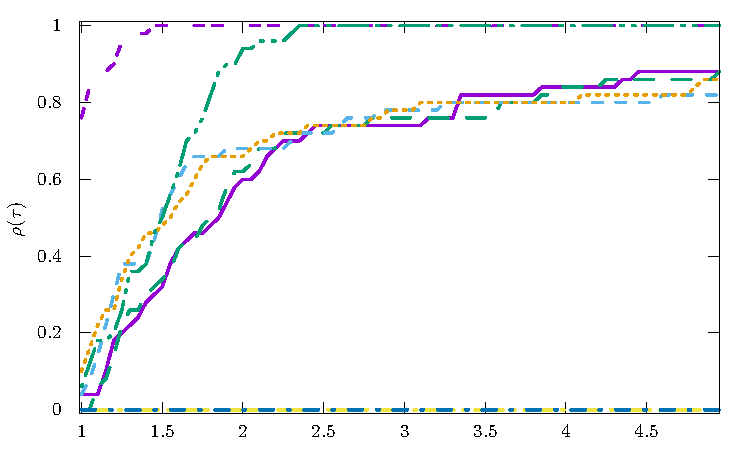
\includegraphics[width=\figwidth]{../figure/NSGS/LocalSolver/1.0e-04/400/time/profile-LMGC_LowWall_FEM.pdf}}
    \subfloat[\scriptsize Cubes\_H8 II]
    {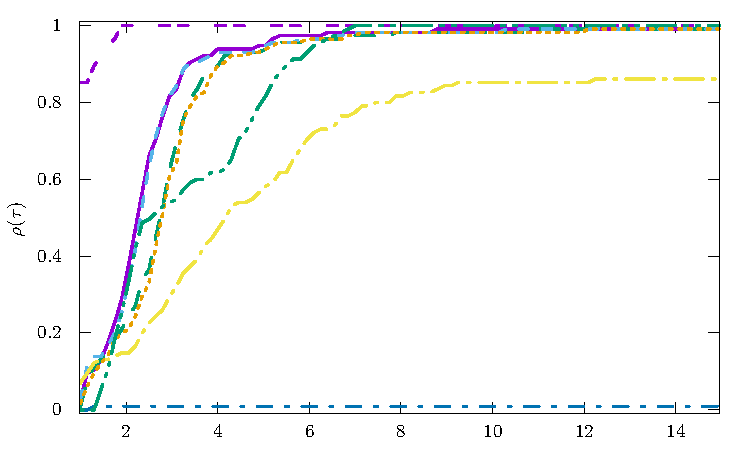
\includegraphics[width=\figwidth]{../figure/NSGS/LocalSolver/1.0e-04/100/time/profile-LMGC_Cubes_H8.pdf}} \\
    \subfloat[\scriptsize Cubes\_H8]
    {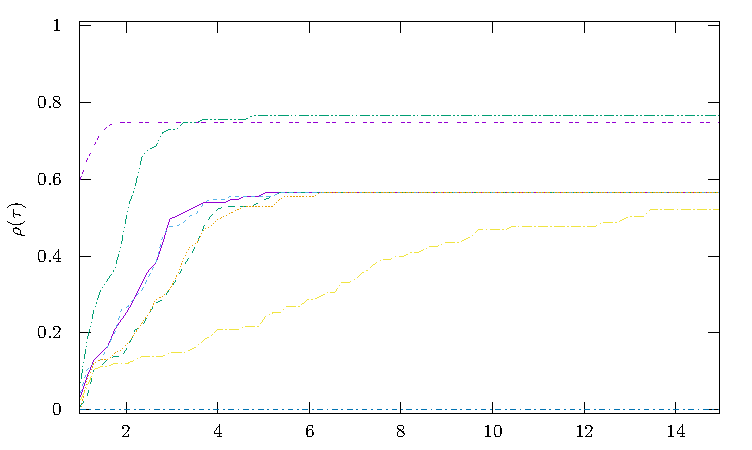
\includegraphics[width=\figwidth]{../figure/NSGS/LocalSolver/1.0e-08/100/time/profile-LMGC_Cubes_H8.pdf}}
    \subfloat[\scriptsize Bridge\_PR II]
    {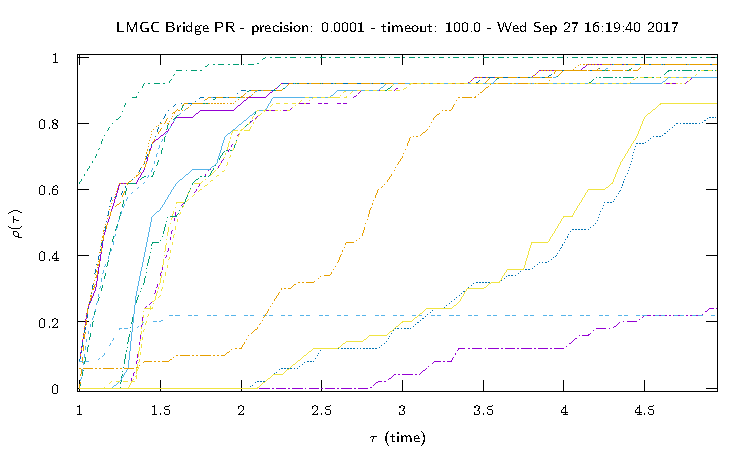
\includegraphics[width=\figwidth]{../figure/NSGS/LocalSolver/1.0e-04/100/time/profile-LMGC_Bridge_PR.pdf}} \\
    \subfloat[\scriptsize Bridge\_PR]
    {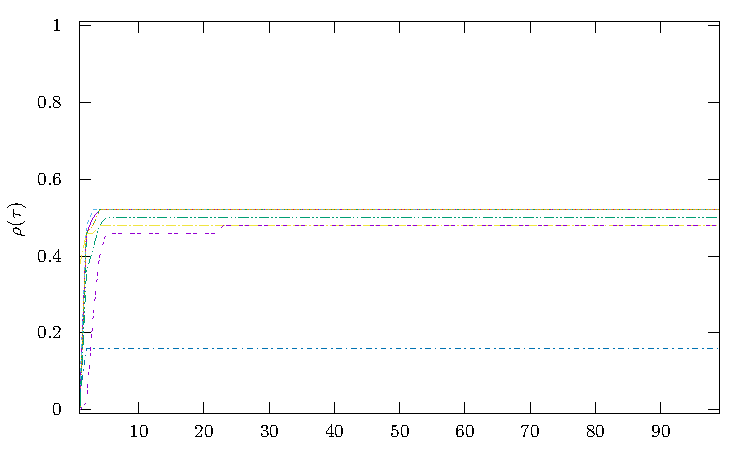
\includegraphics[width=\figwidth]{../figure/NSGS/LocalSolver/1.0e-08/400/time/profile-LMGC_Bridge_PR.pdf}}
    \subfloat[\scriptsize AqueducPR]
    {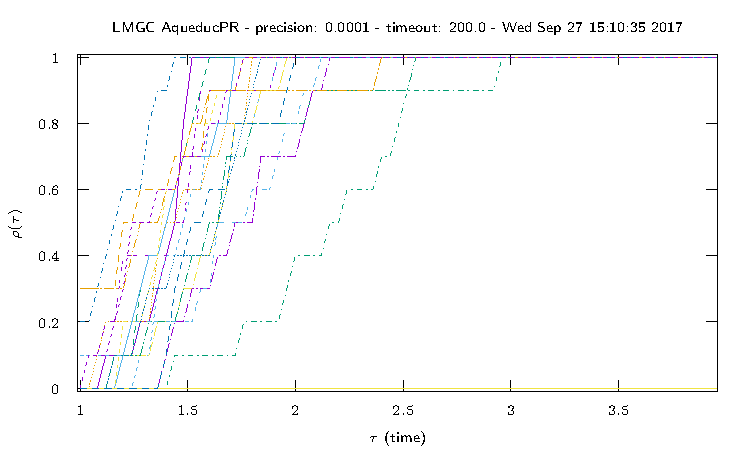
\includegraphics[width=\figwidth]{../figure/NSGS/LocalSolver/1.0e-04/200/time/profile-LMGC_AqueducPR.pdf}}\\
    \subfloat[\scriptsize 945\_SP\_Box\_PL]
    {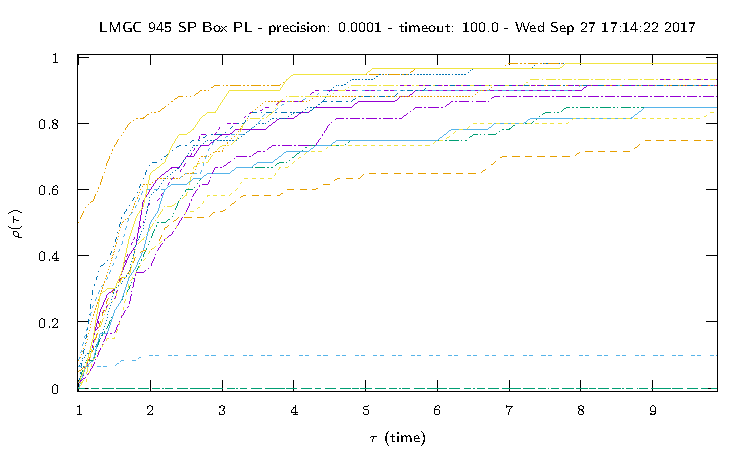
\includegraphics[width=\figwidth]{../figure/NSGS/LocalSolver/1.0e-04/100/time/profile-LMGC_945_SP_Box_PL.pdf}}
    \subfloat[\scriptsize 100\_PR\_PerioBox]
    {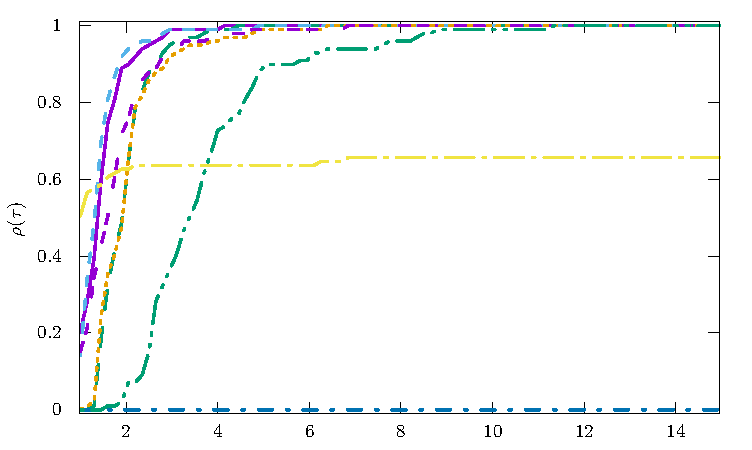
\includegraphics[width=\figwidth]{../figure/NSGS/LocalSolver/1.0e-04/100/time/profile-LMGC_100_PR_PerioBox.pdf}} \\
    \caption{Influence of the local solver in {\sf NSGS-$\star$} algorithms.}
  \end{figure}
  \begin{figure}
    \centering
    \ContinuedFloat
    \subfiglayout
    \subfloat[\scriptsize KaplasTower II]
    {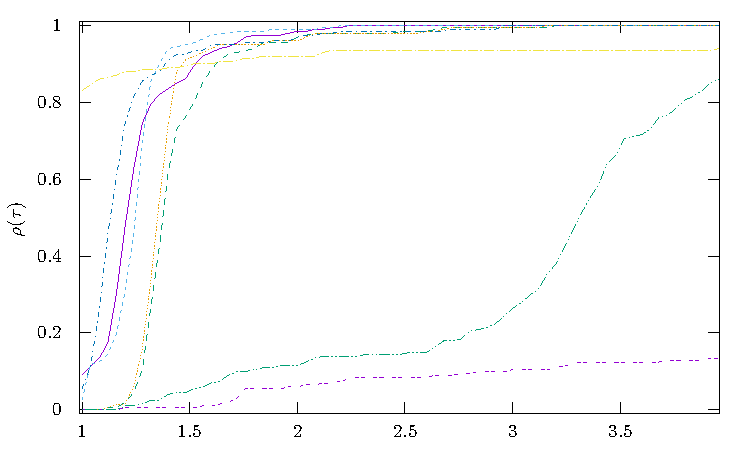
\includegraphics[width=\figwidth]{../figure/NSGS/LocalSolver/1.0e-04/100/time/profile-KaplasTower.pdf}}
    \subfloat[\scriptsize KaplasTower]
    {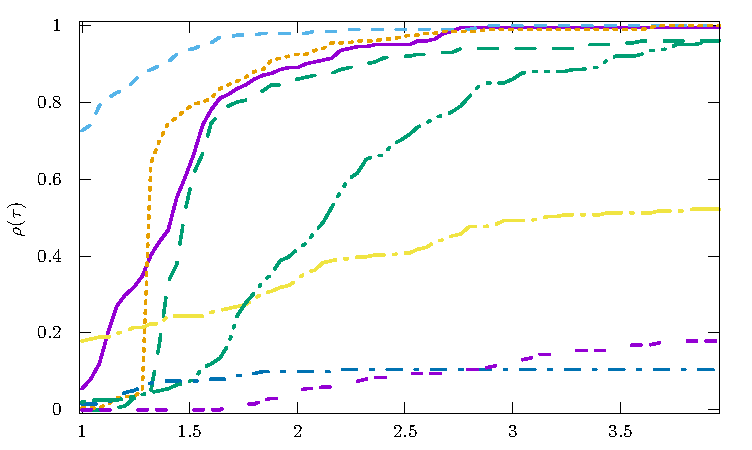
\includegraphics[width=\figwidth]{../figure/NSGS/LocalSolver/1.0e-08/200/time/profile-KaplasTower.pdf}} \\
    \subfloat[\scriptsize Chute\_local\_problems]
    {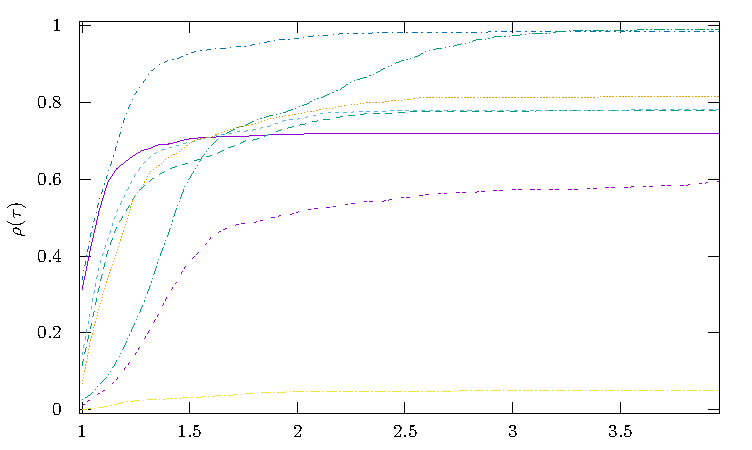
\includegraphics[width=\figwidth]{../figure/NSGS/LocalSolver/1.0e-08/10/time/profile-Chute_local_problems.pdf}}
    \subfloat[\scriptsize Chute\_4000]
    {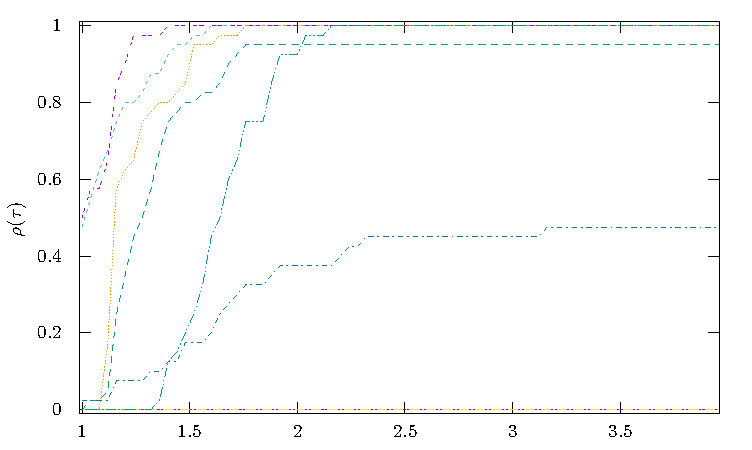
\includegraphics[width=\figwidth]{../figure/NSGS/LocalSolver/1.0e-04/200/time/profile-Chute_4000.pdf}} \\
    \subfloat[\scriptsize Chute\_1000]
    {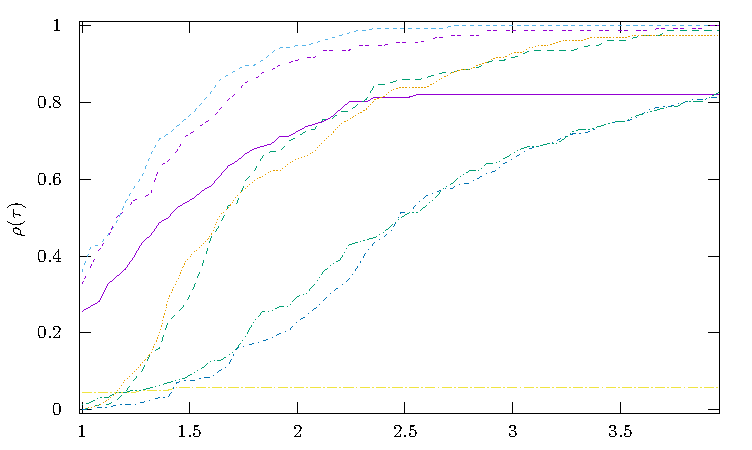
\includegraphics[width=\figwidth]{../figure/NSGS/LocalSolver/1.0e-04/200/time/profile-Chute_1000.pdf}}
    \subfloat[\scriptsize Chain]
    {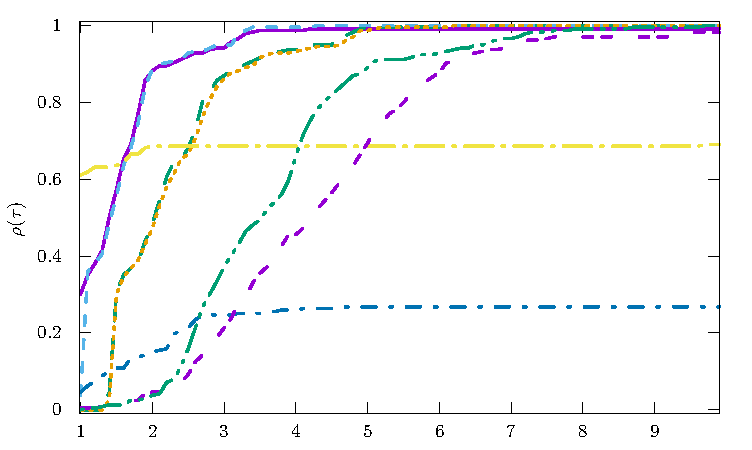
\includegraphics[width=\figwidth]{../figure/NSGS/LocalSolver/1.0e-08/50/time/profile-Chain.pdf}} \\
    \subfloat[\scriptsize Capsules]
    {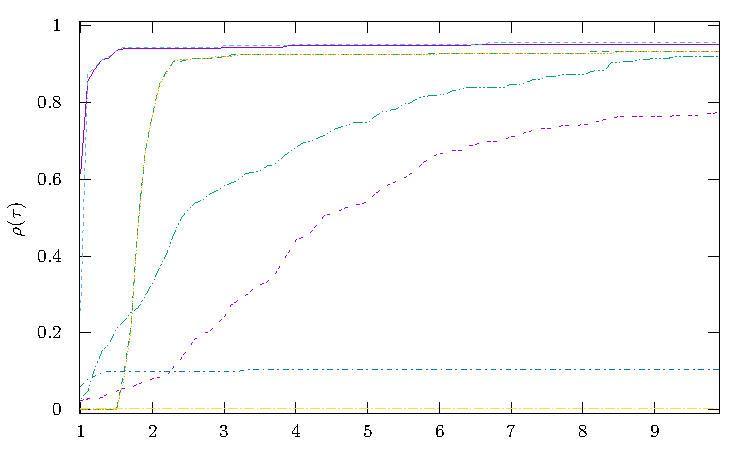
\includegraphics[width=\figwidth]{../figure/NSGS/LocalSolver/1.0e-08/50/time/profile-Capsules.pdf}}
    \subfloat[\scriptsize BoxesStack]
    {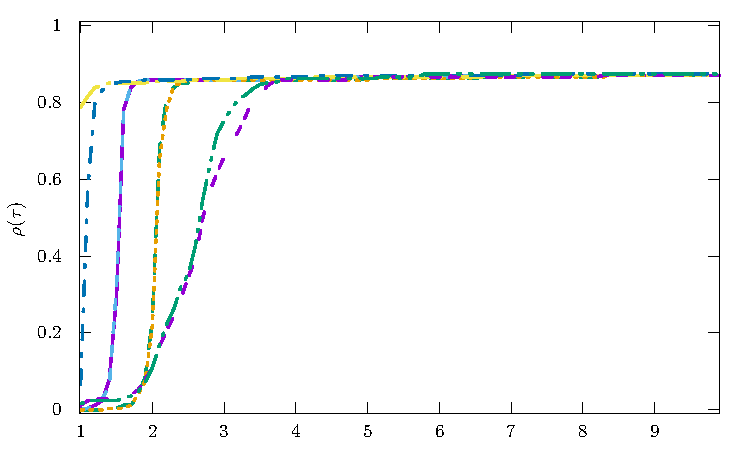
\includegraphics[width=\figwidth]{../figure/NSGS/LocalSolver/1.0e-08/100/time/profile-BoxesStack1.pdf}} \\
    {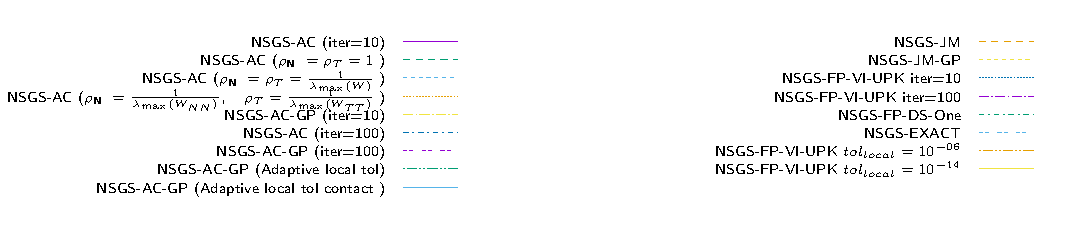
\includegraphics[height=\legendheight]{../figure/NSGS/LocalSolver/1.0e-08/50/time/profile-Chain_legend.pdf}}
    \caption{Influence of the local solver in {\sf NSGS-$\star$} algorithms (continued).}
    \label{fig:NSGS/LocalSolver}
  \end{figure}

\paragraph{Influence of the tolerance of the local solver $\sf tol_{local}$ in {\sf NSGS-FP-VI-UPK} algorithms}
In this paragraph, the tolerance of the local solver $\sf tol_{local}$  is varied and its effect on the global convergence of the solver is reported. In Figure~\ref{fig:NSGS/LocalTol/VI},  we report the performance profiles of {\sf NSGS-FP-VI-UPK} algorithms for the $\sf tol_{local}$ in the range $[10^{-04}, 10^{-16}]$. We also report the efficiency of the adaptive strategy for setting the value of the local tolerance (see Section~\ref{Sec:NSGS-LocalTol}). The main observations are:
\begin{enumerate}
\item For the test sets that are quickly solved (see Table~\ref{Tab:fclib-simulation}), such as   Capsules  a tight tolerance on the local solver $10^{-16}$ improves the efficiency  of the {\sf NSGS-FP-VI-UPK} solver. Similar results are obtained for BoxesStack, Chain, KaplasTower and KaplasTower II; they are not depicted. 
\item For the other problems that are longer to solve, that is, when we expect more iterations of the  {\sf NSGS-FP-VI-UPK} solver, the adaptive rule, or a tight local tolerance is better.
\end{enumerate}
From these results, it is quite difficult to guess in advance the internal dynamics of the solver. By internal dynamics, we mean the propagation in the algorithm between the local problem and the global loop. Note that the range of $\tau$ that we used in the graph is quite small so the difference in performance between the solvers is not crucial.

\begin{figure}
  \centering
    \subfiglayout
\subfloat[\scriptsize LowWall\_FEM]
   {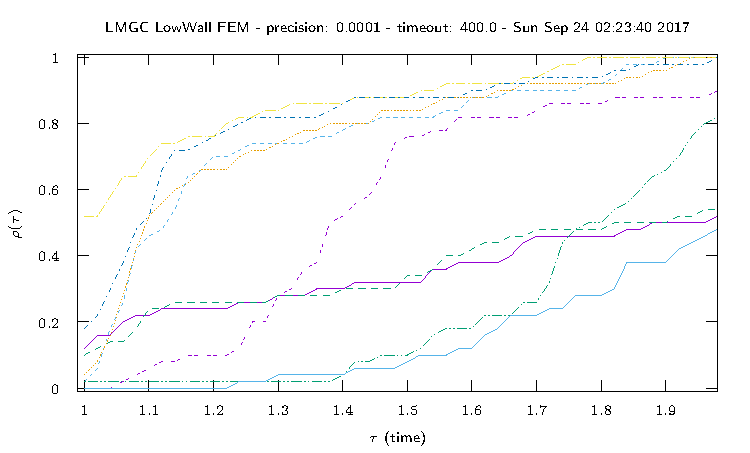
\includegraphics[width=\figwidth]{../figure/NSGS/LocalTol/VI/1.0e-04/400/time/profile-LMGC_LowWall_FEM.pdf}} 
\subfloat[\scriptsize Cubes\_H8 II]
   {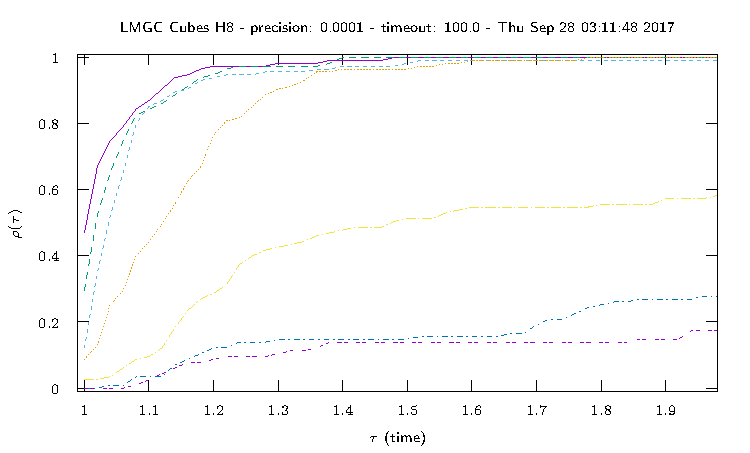
\includegraphics[width=\figwidth]{../figure/NSGS/LocalTol/VI/1.0e-04/100/time/profile-LMGC_Cubes_H8.pdf}} \\
% \subfloat[\scriptsize Cubes\_H8]
%    {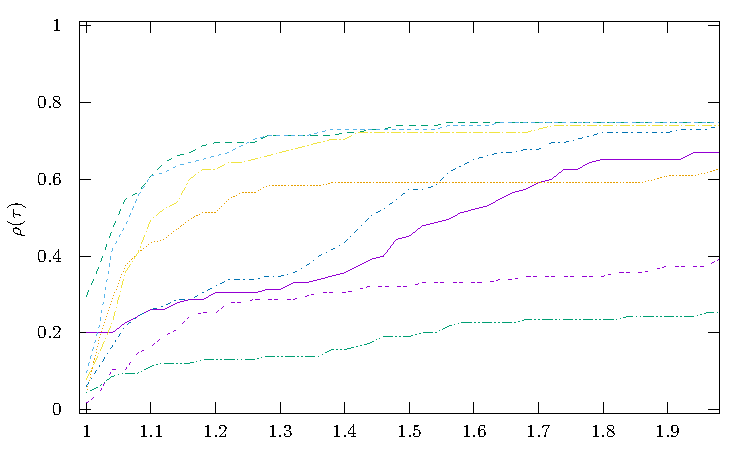
\includegraphics[width=\figwidth]{../figure/NSGS/LocalTol/VI/1.0e-08/100/time/profile-LMGC_Cubes_H8.pdf}} \\
\subfloat[\scriptsize Bridge\_PR II]
   {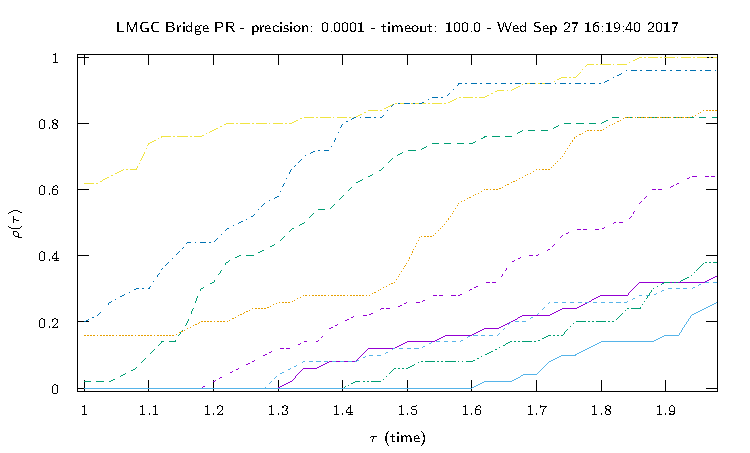
\includegraphics[width=\figwidth]{../figure/NSGS/LocalTol/VI/1.0e-04/100/time/profile-LMGC_Bridge_PR.pdf}} 
% \subfloat[\scriptsize Bridge\_PR]
%    {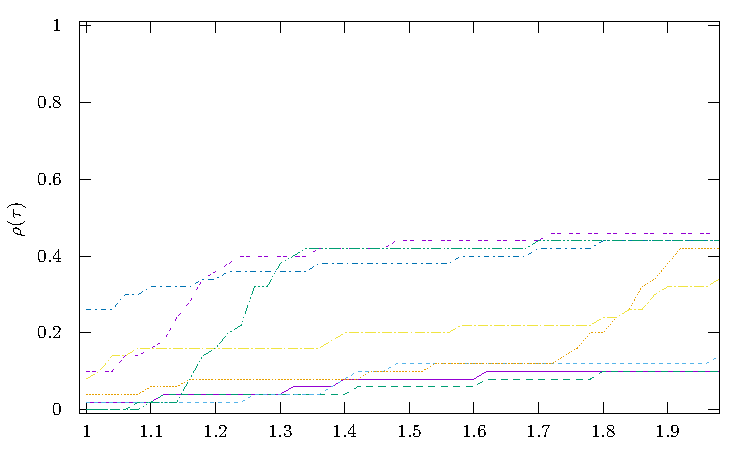
\includegraphics[width=\figwidth]{../figure/NSGS/LocalTol/VI/1.0e-08/400/time/profile-LMGC_Bridge_PR.pdf}}
% \subfloat[\scriptsize AqueducPR]
%    {\includegraphics[width=\figwidth]{../figure/NSGS/LocalTol/VI/1.0e-04/200/time/profile-LMGC_AqueducPR.pdf}}
% \subfloat[\scriptsize 945\_SP\_Box\_PL]
%    {\includegraphics[width=\figwidth]{../figure/NSGS/LocalTol/VI/1.0e-04/100/time/profile-LMGC_945_SP_Box_PL.pdf}} \\
   \subfloat[\scriptsize 100\_PR\_PerioBox]
    {\includegraphics[width=\figwidth]{../figure/NSGS/LocalTol/VI/1.0e-04/100/time/profile-LMGC_100_PR_PerioBox.pdf}} \\
% \subfloat[\scriptsize KaplasTower II]
%    {\includegraphics[width=\figwidth]{../figure/NSGS/LocalTol/VI/1.0e-04/100/time/profile-KaplasTower.pdf}} 
% \subfloat[\scriptsize KaplasTower]
%    {\includegraphics[width=\figwidth]{../figure/NSGS/LocalTol/VI/1.0e-08/200/time/profile-KaplasTower.pdf}} \\
\subfloat[\scriptsize Chute\_local\_problems]
    {\includegraphics[width=\figwidth]{../figure/NSGS/LocalTol/VI/1.0e-08/10/time/profile-Chute_local_problems.pdf}}
\subfloat[\scriptsize Chute\_4000]
   {\includegraphics[width=\figwidth]{../figure/NSGS/LocalTol/VI/1.0e-04/200/time/profile-Chute_4000.pdf}} \\
\subfloat[\scriptsize Chute\_1000]
    {\includegraphics[width=\figwidth]{../figure/NSGS/LocalTol/VI/1.0e-04/200/time/profile-Chute_1000.pdf}} 
% \subfloat[\scriptsize Chain]
%   {\includegraphics[width=\figwidth]{../figure/NSGS/LocalTol/VI/1.0e-08/50/time/profile-Chain.pdf}} 
\subfloat[\scriptsize Capsules]
   {\includegraphics[width=\figwidth]{../figure/NSGS/LocalTol/VI/1.0e-08/50/time/profile-Capsules.pdf}} 
% \subfloat[\scriptsize BoxesStack]
% {\includegraphics[width=\figwidth]{../figure/NSGS/LocalTol/VI/1.0e-08/100/time/profile-BoxesStack1.pdf}}
\\
{\includegraphics[width=\legendwidth]{../figure/NSGS/LocalTol/VI/1.0e-08/50/time/profile-Chain_legend.pdf}} 
\caption{Influence of the tolerance of the local solver $\sf tol_{local}$ in {\sf NSGS-FP-VI-UPK} algorithms.}
 \label{fig:NSGS/LocalTol/VI}
\end{figure}

\paragraph{Influence of the tolerance of the local solver $\sf tol_{local}$ in {\sf NSGS-AC-GP} algorithms.}
In Figure~\ref{fig:NSGS/LocalTol},  we report the performance profiles of {\sf NSGS-AC-GP} algorithms for the $\sf tol_{local}$ in the range $[10^{-04}, 10^{-16}]$. We also test the  adaptive strategy value for the local tolerance. Except for the test set Chute\_local\_problems,  the main observation is that the local tolerance does not change fundamentally the convergence of the solver. For the test set Chute\_local\_problems, there is no internal dynamics of the main loop of the {\sf NSGS} since there is only one contact. It is therefore reasonable to see that adaptive strategy performs better that the other.



\begin{figure}
  \centering
    \subfiglayout
\subfloat[\scriptsize LowWall\_FEM]
   {\includegraphics[width=\figwidth]{../figure/NSGS/LocalTol/1.0e-04/400/time/profile-LMGC_LowWall_FEM.pdf}} 
\subfloat[\scriptsize Cubes\_H8 II]
   {\includegraphics[width=\figwidth]{../figure/NSGS/LocalTol/1.0e-04/100/time/profile-LMGC_Cubes_H8.pdf}} \\
% \subfloat[\scriptsize Cubes\_H8]
%    {\includegraphics[width=\figwidth]{../figure/NSGS/LocalTol/1.0e-08/100/time/profile-LMGC_Cubes_H8.pdf}} 
% \subfloat[\scriptsize Bridge\_PR II]
%    {\includegraphics[width=\figwidth]{../figure/NSGS/LocalTol/1.0e-04/100/time/profile-LMGC_Bridge_PR.pdf}} 
% \subfloat[\scriptsize Bridge\_PR]
%    {\includegraphics[width=\figwidth]{../figure/NSGS/LocalTol/1.0e-08/400/time/profile-LMGC_Bridge_PR.pdf}} 
% \subfloat[\scriptsize AqueducPR]
%    {\includegraphics[width=\figwidth]{../figure/NSGS/LocalTol/1.0e-04/200/time/profile-LMGC_AqueducPR.pdf}} \\
% \subfloat[\scriptsize 945\_SP\_Box\_PL]
%    {\includegraphics[width=\figwidth]{../figure/NSGS/LocalTol/1.0e-04/100/time/profile-LMGC_945_SP_Box_PL.pdf}} \\
% \subfloat[\scriptsize 100\_PR\_PerioBox]
%    {\includegraphics[width=\figwidth]{../figure/NSGS/LocalTol/1.0e-04/100/time/profile-LMGC_100_PR_PerioBox.pdf}}
% \subfloat[\scriptsize KaplasTower II]
%    {\includegraphics[width=\figwidth]{../figure/NSGS/LocalTol/1.0e-04/100/time/profile-KaplasTower.pdf}} 
% \subfloat[\scriptsize KaplasTower]
%    {\includegraphics[width=\figwidth]{../figure/NSGS/LocalTol/1.0e-08/200/time/profile-KaplasTower.pdf}} 
\subfloat[\scriptsize Chute\_local\_problems]
   {\includegraphics[width=\figwidth]{../figure/NSGS/LocalTol/1.0e-08/10/time/profile-Chute_local_problems.pdf}} 
\subfloat[\scriptsize Chute\_4000]
   {\includegraphics[width=\figwidth]{../figure/NSGS/LocalTol/1.0e-04/200/time/profile-Chute_4000.pdf}} 
% \subfloat[\scriptsize Chute\_1000]
%    {\includegraphics[width=\figwidth]{../figure/NSGS/LocalTol/1.0e-04/200/time/profile-Chute_1000.pdf}} \\
% \subfloat[\scriptsize Chain]
%    {\includegraphics[width=\figwidth]{../figure/NSGS/LocalTol/1.0e-08/50/time/profile-Chain.pdf}} 
% \subfloat[\scriptsize Capsules]
%    {\includegraphics[width=\figwidth]{../figure/NSGS/LocalTol/1.0e-08/50/time/profile-Capsules.pdf}} 
% \subfloat[\scriptsize BoxesStack]
% {\includegraphics[width=\figwidth]{../figure/NSGS/LocalTol/1.0e-08/100/time/profile-BoxesStack1.pdf}}
   \\
{\includegraphics[width=\legendwidth]{../figure/NSGS/LocalTol/1.0e-08/50/time/profile-Chain_legend.pdf}} 
\caption{Influence of the tolerance of the local solver $\sf tol_{local}$ in {\sf NSGS-FP-NSN-AC-GP} algorithms.}
\label{fig:NSGS/LocalTol}
\end{figure}

\paragraph{Influence of the choice of the parameters $\rho_\n, \rho_\t$ in the local solver of the {\sf NSGS-AC} algorithms}

In Figure~\ref{fig:NSGS/rho}, we evaluate the influence of the choice of the parameters $\rho_\n, \rho_\t$ on the convergence of the solver. The main conclusion are:
\begin{enumerate}
\item For the test sets 945\_SP\_Box\_PL, 100\_PR\_PerioBox, KaplasTower II, KaplasTower, Chute\_local\_problems, Chute\_4000, Chute\_1000, Capsules, a fixed value of $\rho_\n=\rho_\t=1$ has a dramatic effect on the convergence of the algorithm. The scaling of $\rho$ is of utmost importance for the efficiency and the robustness of the solver. Note that the rule  \eqref{eq:rho-4} that takes into account the condition number of the local Delassus matrix $W$ deteriorates the performance for  Chute\_4000, Chute\_1000. In these problems, the local matrix is unsymmetric with large extra-diagonal terms due to large gyroscopic effects.
  
\item For the other tests, the choice of $\rho_\n,\rho_\t$ does not really change the results such as LowWall\_FEM, mainly due the fact that the order of magnitude of the chosen $\rho$ with the rules \eqref{eq:rho-2}, \eqref{eq:rho-3} or \eqref{eq:rho-4} is in $[10^{-01}, 1]$. Cubes\_H8 II, Cubes\_H8, Bridge\_PR II, Bridge\_PR, 100\_PR\_PerioBox, Chain, BoxesStack and AqueducPR are not displayed since the results are similar.
\end{enumerate}
One of the conclusion of this study is as follows, the rules \eqref{eq:rho-2}, \eqref{eq:rho-3} improves a lot some simulations without increasing the computational cost for the others. Therefore, it is strongly advised to use it. Some further theoretical studies are needed to understand the effect of $\rho$ on the convergence. In particular, the rule \eqref{eq:rho-4} is usually better, but sometimes destroy completely the convergence.
\begin{figure}
  \centering
    \subfiglayout
\subfloat[\scriptsize LowWall\_FEM]
   {\includegraphics[width=\figwidth]{../figure/NSGS/rho/1.0e-04/400/time/profile-LMGC_LowWall_FEM.pdf}}
% \subfloat[\scriptsize Cubes\_H8 II]
%    {\includegraphics[width=\figwidth]{../figure/NSGS/rho/1.0e-04/100/time/profile-LMGC_Cubes_H8.pdf}}
% \subfloat[\scriptsize Cubes\_H8]
%    {\includegraphics[width=\figwidth]{../figure/NSGS/rho/1.0e-08/100/time/profile-LMGC_Cubes_H8.pdf}} \\
% \subfloat[\scriptsize Bridge\_PR II]
%    {\includegraphics[width=\figwidth]{../figure/NSGS/rho/1.0e-04/100/time/profile-LMGC_Bridge_PR.pdf}}
% \subfloat[\scriptsize Bridge\_PR]
%    {\includegraphics[width=\figwidth]{../figure/NSGS/rho/1.0e-08/400/time/profile-LMGC_Bridge_PR.pdf}}
% \subfloat[\scriptsize AqueducPR]
%    {\includegraphics[width=\figwidth]{../figure/NSGS/rho/1.0e-04/200/time/profile-LMGC_AqueducPR.pdf}} \\
\subfloat[\scriptsize 945\_SP\_Box\_PL]
   {\includegraphics[width=\figwidth]{../figure/NSGS/rho/1.0e-04/100/time/profile-LMGC_945_SP_Box_PL.pdf}} \\
% \subfloat[\scriptsize 100\_PR\_PerioBox]
%    {\includegraphics[width=\figwidth]{../figure/NSGS/rho/1.0e-08/200/time/profile-LMGC_100_PR_PerioBox.pdf}} \\
\subfloat[\scriptsize KaplasTower II]
   {\includegraphics[width=\figwidth]{../figure/NSGS/rho/1.0e-04/100/time/profile-KaplasTower.pdf}} 
\subfloat[\scriptsize KaplasTower]
   {\includegraphics[width=\figwidth]{../figure/NSGS/rho/1.0e-08/200/time/profile-KaplasTower.pdf}} \\
\subfloat[\scriptsize Chute\_local\_problems]
   {\includegraphics[width=\figwidth]{../figure/NSGS/rho/1.0e-08/10/time/profile-Chute_local_problems.pdf}}
\subfloat[\scriptsize Chute\_4000]
   {\includegraphics[width=\figwidth]{../figure/NSGS/rho/1.0e-04/200/time/profile-Chute_4000.pdf}}\\
\subfloat[\scriptsize Chute\_1000]
   {\includegraphics[width=\figwidth]{../figure/NSGS/rho/1.0e-04/200/time/profile-Chute_1000.pdf}} 
% \subfloat[\scriptsize Chain]
%    {\includegraphics[width=\figwidth]{../figure/NSGS/rho/1.0e-08/50/time/profile-Chain.pdf}}
\subfloat[\scriptsize Capsules]
   {\includegraphics[width=\figwidth]{../figure/NSGS/rho/1.0e-08/50/time/profile-Capsules.pdf}}\\
% \subfloat[\scriptsize BoxesStack]
%    {\includegraphics[width=\figwidth]{../figure/NSGS/rho/1.0e-08/100/time/profile-BoxesStack1.pdf}} \\
{\includegraphics[height=\legendheight]{../figure/NSGS/rho/1.0e-08/50/time/profile-Chain_legend.pdf}}
  \caption{Influence of the choice of the parameters $\rho_\n, \rho_\t$ in the local solver of the {\sf NSGS-AC} algorithms }
  \label{fig:NSGS/rho}
\end{figure}



\paragraph{Influence of the contacts order  in NSGS algorithms}
In this section, we study the influence of the contact order within the loop of the {\sf NSGS-AC-GP} solver. We reproduce in Figure~\ref{fig:NSGS/Shuffled} the result of the solvers with the original contact list of the problem ({\sf NSGS-AC-GP}) and with two other ways of iterating over the contacts. The solver {\sf NSGS-AC-GP Shuffled} corresponds to a single randomization of the list of contacts at the beginning of the algorithm. In the solver  {\sf NSGS-AC-GP Fully shuffled}, the  list is shuffled at each iteration. The following observations can be made:
\begin{enumerate}
\item The solver  {\sf NSGS-AC-GP Fully shuffled} performs really better on the flexible test sets
\item For the rigid test sets, we reproduce here only the test set  100\_PR\_PerioBox because the other test sets behave similarly. The  {\sf NSGS-AC-GP Fully shuffled} has a really bad influence on the convergence of the solver. It seems that it modifies the internal dynamics of the solver in a way that the rate of convergence is really decreased.
\end{enumerate}
\begin{figure}
  \centering
    \subfiglayout
  \subfloat[\scriptsize LowWall\_FEM]
   {\includegraphics[width=\figwidth]{../figure/NSGS/Shuffled/1.0e-04/400/time/profile-LMGC_LowWall_FEM.pdf}} 
   \subfloat[\scriptsize Cubes\_H8 II]
   {\includegraphics[width=\figwidth]{../figure/NSGS/Shuffled/1.0e-04/100/time/profile-LMGC_Cubes_H8.pdf}} \\
% \subfloat[\scriptsize Cubes\_H8]
%    {\includegraphics[width=\figwidth]{../figure/NSGS/Shuffled/1.0e-08/100/time/profile-LMGC_Cubes_H8.pdf}} \\
\subfloat[\scriptsize Bridge\_PR II]
   {\includegraphics[width=\figwidth]{../figure/NSGS/Shuffled/1.0e-04/100/time/profile-LMGC_Bridge_PR.pdf}}  
% \subfloat[\scriptsize Bridge\_PR]
%    {\includegraphics[width=\figwidth]{../figure/NSGS/Shuffled/1.0e-08/400/time/profile-LMGC_Bridge_PR.pdf}} 
% \subfloat[\scriptsize AqueducPR]
%    {\includegraphics[width=\figwidth]{../figure/NSGS/Shuffled/1.0e-04/200/time/profile-LMGC_AqueducPR.pdf}} \\
% \subfloat[\scriptsize 945\_SP\_Box\_PL]
%    {\includegraphics[width=\figwidth]{../figure/NSGS/Shuffled/1.0e-04/100/time/profile-LMGC_945_SP_Box_PL.pdf}} 
\subfloat[\scriptsize 100\_PR\_PerioBox]
   {\includegraphics[width=\figwidth]{../figure/NSGS/Shuffled/1.0e-04/100/time/profile-LMGC_100_PR_PerioBox.pdf}} \\
% \subfloat[\scriptsize KaplasTower II]
%    {\includegraphics[width=\figwidth]{../figure/NSGS/Shuffled/1.0e-04/100/time/profile-KaplasTower.pdf}} 
% \subfloat[\scriptsize KaplasTower]
%    {\includegraphics[width=\figwidth]{../figure/NSGS/Shuffled/1.0e-08/200/time/profile-KaplasTower.pdf}} 
% \subfloat[\scriptsize Chute\_local\_problems]
%    {\includegraphics[width=\figwidth]{../figure/NSGS/Shuffled/1.0e-08/10/time/profile-Chute_local_problems.pdf}} 
% \subfloat[\scriptsize Chute\_4000]
%    {\includegraphics[width=\figwidth]{../figure/NSGS/Shuffled/1.0e-04/200/time/profile-Chute_4000.pdf}} 
% \subfloat[\scriptsize Chute\_1000]
%    {\includegraphics[width=\figwidth]{../figure/NSGS/Shuffled/1.0e-04/200/time/profile-Chute_1000.pdf}} \\
% \subfloat[\scriptsize Chain]
%    {\includegraphics[width=\figwidth]{../figure/NSGS/Shuffled/1.0e-08/50/time/profile-Chain.pdf}} 
% \subfloat[\scriptsize Capsules]
% {\includegraphics[width=\figwidth]{../figure/NSGS/Shuffled/1.0e-08/50/time/profile-Capsules.pdf}}
   % \subfloat[\scriptsize BoxesStack]
   % {\includegraphics[width=\figwidth]{../figure/NSGS/Shuffled/1.0e-08/100/time/profile-BoxesStack1.pdf}}
{\includegraphics[height=\legendheight]{../figure/NSGS/Shuffled/1.0e-08/50/time/profile-Chain_legend.pdf}} 
\caption{Influence of the contacts order in NSGS algorithms.}
\label{fig:NSGS/Shuffled}
\end{figure}

\paragraph{Comparison of {\sf PSOR}  algorithm with respect to  the relaxation parameter $\omega$}

In Figure~\ref{fig:PSOR},  the relaxation parameter $\omega$ is varied ranging in $[0.5,1.8]$.  Two conclusions can be drawn:
\begin{enumerate}
\item For the flexible tests, the efficiency of the solver is really improved as we decreased the value of $\omega$. Moreover, this is done without destroying the robustness of the solver.
\item For the rigid tests, the effect of the relaxation is not so clear. For values of $\omega$ greater than $1.0$, the efficiency is improved but the robustness deteriorates and we observe the contrary for the  $\omega$  less than $1.0$. Note in particular that for the test sets Chute\_1000, Chute\_4000 the convergence is completely destroyed for $\omega = 1.8$.
\end{enumerate}
To conclude, it is difficult to advice to use PSOR algorithm with $\omega\neq 1$. If it accelerates drastically the rate of convergence of the algorithm for some problems, but it deteriorates the convergence for others. Further studies would be needed to design self--adaptive schemes for sizing $\omega$.

% \begin{ndrva}
%   \item redo this comparison on a set of mixed examples
%   \item add some results with $\omega =1.8$ to show that higher values will destroy the convergence.
%   \item is it possible to find sizing rule in the literature ?
% \end{ndrva}
\begin{figure}
  \centering
    \subfiglayout
  \subfloat[\scriptsize LowWall\_FEM]
   {\includegraphics[width=\figwidth]{../figure/PSOR/1.0e-04/400/time/profile-LMGC_LowWall_FEM.pdf}} 
\subfloat[\scriptsize Cubes\_H8 II]
   {\includegraphics[width=\figwidth]{../figure/PSOR/1.0e-04/100/time/profile-LMGC_Cubes_H8.pdf}} 
% \subfloat[\scriptsize Cubes\_H8]
%    {\includegraphics[width=\figwidth]{../figure/PSOR/1.0e-08/100/time/profile-LMGC_Cubes_H8.pdf}}
   \\
% \subfloat[\scriptsize Bridge\_PR II]
%    {\includegraphics[width=\figwidth]{../figure/PSOR/1.0e-04/100/time/profile-LMGC_Bridge_PR.pdf}}
% \subfloat[\scriptsize Bridge\_PR]
%    {\includegraphics[width=\figwidth]{../figure/PSOR/1.0e-08/400/time/profile-LMGC_Bridge_PR.pdf}}
% \subfloat[\scriptsize AqueducPR]
%    {\includegraphics[width=\figwidth]{../figure/PSOR/1.0e-04/200/time/profile-LMGC_AqueducPR.pdf}} \\
% \subfloat[\scriptsize 945\_SP\_Box\_PL]
%    {\includegraphics[width=\figwidth]{../figure/PSOR/1.0e-04/100/time/profile-LMGC_945_SP_Box_PL.pdf}}
% \subfloat[\scriptsize 100\_PR\_PerioBox]
%    {\includegraphics[width=\figwidth]{../figure/PSOR/1.0e-04/100/time/profile-LMGC_100_PR_PerioBox.pdf}}
% \subfloat[\scriptsize KaplasTower II]
%    {\includegraphics[width=\figwidth]{../figure/PSOR/1.0e-04/100/time/profile-KaplasTower.pdf}}
% \subfloat[\scriptsize KaplasTower]
%    {\includegraphics[width=\figwidth]{../figure/PSOR/1.0e-08/200/time/profile-KaplasTower.pdf}}
% \subfloat[\scriptsize Chute\_local\_problems]
%    {\includegraphics[width=\figwidth]{../figure/PSOR/1.0e-08/10/time/profile-Chute_local_problems.pdf}} \\
\subfloat[\scriptsize Chute\_4000]
   {\includegraphics[width=\figwidth]{../figure/PSOR/1.0e-04/200/time/profile-Chute_4000.pdf}} 
\subfloat[\scriptsize Chute\_1000]
   {\includegraphics[width=\figwidth]{../figure/PSOR/1.0e-04/200/time/profile-Chute_1000.pdf}} \\
\subfloat[\scriptsize Chain]
   {\includegraphics[width=\figwidth]{../figure/PSOR/1.0e-08/50/time/profile-Chain.pdf}} 
\subfloat[\scriptsize Capsules]
   {\includegraphics[width=\figwidth]{../figure/PSOR/1.0e-08/50/time/profile-Capsules.pdf}} 
% \subfloat[\scriptsize BoxesStack]
% {\includegraphics[width=\figwidth]{../figure/PSOR/1.0e-08/100/time/profile-BoxesStack1.pdf}}
\\
{\includegraphics[height=\legendheight]{../figure/PSOR/1.0e-08/50/time/profile-Chain_legend.pdf}} 
  \caption{Effect of relation coefficient $\omega$ in {\sf PSOR-AC-GP} algorithm.}
  \label{fig:PSOR}
\end{figure}

\subsection{Comparison of {\sf NSN-$\star$} algorithms}

In this section,  the nonsmooth Newton methods  are compared.  The performance profiles are depicted in Figure~\ref{fig:NSN} for the test sets for which the {\sf NSN-$\star$} are able to solve at least 10\% of the problems. The main conclusion are as follows:
\begin{enumerate}
\item For the flexible tests, most of the Newton methods succeed to solve the problems within the prescribed time limit. The solver {\sf NSN-AC-HYBRID} appears to be the best solver.  The effect of computing an initial condition of the solver with a robust method such as {\sf EG-VI-UPK}  improves the convergence. In practice, we observe that the precomputation allows one to determine roughly the set of closed and sliding contacts and it helps a lot the convergence of the Newton solvers. The solvers without line--searches perform also better than those with a line--search procedure which  seems to slow down the convergence without improving the robustness.  For the different formulations, the {\sf NSN-AC} and {\sf NSN-JM} give equivalent results and are better that the {\sf NSN-NM} solver which is in turns better than the {\sf NSN-FB} solver. Note that the Goldstein--Price line search is usually better than the Armijo despite the fact the merit function is not necessarily smooth. Finally, we note that  {\sf NSN-FB}  and {\sf NSN-FB-A} are really the slowest solver on these flexible examples.
\item For the rigid test sets with an high value of the rank ratio or the contact density~$c$ (see Table~\ref{Tab:fclib}), the Newton methods fail to converge and a lot of divergence has been noted in practice. This is the case for the test sets Bridge\_PR II, Bridge\_PR, AqueducPR, 945\_SP\_Box\_PL, 100\_PR\_PerioBox that are not depicted in Figure~\ref{fig:NSN}.
\item For the rigid test sets with a low value of the rank ratio or the contact density $c$ less than $1$ such as Chute\_1000 and Chain, we observe that the Newton methods are able to solve some problems. We note also that in the Chain test set, the use of a fixed value of $\rho$ is penalizing a lot the convergence of the solver. Contrary to flexible test sets, the use of a line--search procedure helps  to get a better robustness  of the solver. This is particularly true for {\sf NSN-NM-GP}.
\item For the Chute\_local\_problems test set, we observe a large variability of the results depending on the formulation and the line--search procedures.
\item Finally, for the test sets KaplasTower and Capsules, the {\sf NSN-FB-GP} is able to solve more than 80\% in a very efficient way. Some further studies would be needed to understand why this specific solver performs really better than the others.
\end{enumerate}
As general conclusion, the success of the {\sf NSN-$\star$} algorithms is conditioned by  the rank of the Delassus matrix $W$, and then, by the contact density value $c$. For full rank matrix $W$, the solvers are robust and efficient. For values of $c$ not larger than $1$, the methods are able to find a solution with a tight accuracy. For larger values of $c$ and larger rank ratio, the nonsmooth Newton methods are not robust and generally diverge.

\begin{figure}
  \centering
    \subfiglayout
 \subfloat[\scriptsize LowWall\_FEM]
   {\includegraphics[width=\figwidth]{../figure/NSN/1.0e-04/400/time/profile-LMGC_LowWall_FEM.pdf}} 
\subfloat[\scriptsize Cubes\_H8 II]
   {\includegraphics[width=\figwidth]{../figure/NSN/1.0e-04/100/time/profile-LMGC_Cubes_H8.pdf}} \\
\subfloat[\scriptsize Cubes\_H8]
   {\includegraphics[width=\figwidth]{../figure/NSN/1.0e-08/100/time/profile-LMGC_Cubes_H8.pdf}}
% \subfloat[\scriptsize Bridge\_PR II]
%    {\includegraphics[width=\figwidth]{../figure/NSN/1.0e-04/100/time/profile-LMGC_Bridge_PR.pdf}}
% \subfloat[\scriptsize Bridge\_PR]
%    {\includegraphics[width=\figwidth]{../figure/NSN/1.0e-08/400/time/profile-LMGC_Bridge_PR.pdf}}
% \subfloat[\scriptsize AqueducPR]
%    {\includegraphics[width=\figwidth]{../figure/NSN/1.0e-04/200/time/profile-LMGC_AqueducPR.pdf}} \\
% \subfloat[\scriptsize 945\_SP\_Box\_PL]
%    {\includegraphics[width=\figwidth]{../figure/NSN/1.0e-04/100/time/profile-LMGC_945_SP_Box_PL.pdf}}
% \subfloat[\scriptsize 100\_PR\_PerioBox]
% \subfloat[\scriptsize KaplasTower II]
%    {\includegraphics[width=\figwidth]{../figure/NSN/1.0e-04/100/time/profile-KaplasTower.pdf}} \\
\subfloat[\scriptsize KaplasTower]
   {\includegraphics[width=\figwidth]{../figure/NSN/1.0e-08/200/time/profile-KaplasTower.pdf}} \\
\subfloat[\scriptsize Chute\_local\_problems]
   {\includegraphics[width=\figwidth]{../figure/NSN/1.0e-08/10/time/profile-Chute_local_problems.pdf}} 
% \subfloat[\scriptsize Chute\_4000]
%    {\includegraphics[width=\figwidth]{../figure/NSN/1.0e-04/200/time/profile-Chute_4000.pdf}}
\subfloat[\scriptsize Chute\_1000]
   {\includegraphics[width=\figwidth]{../figure/NSN/1.0e-04/200/time/profile-Chute_1000.pdf}} \\
\subfloat[\scriptsize Chain]
   {\includegraphics[width=\figwidth]{../figure/NSN/1.0e-08/50/time/profile-Chain.pdf}} 
\subfloat[\scriptsize Capsules]
   {\includegraphics[width=\figwidth]{../figure/NSN/1.0e-08/50/time/profile-Capsules.pdf}} 
% \subfloat[\scriptsize BoxesStack]
%    {\includegraphics[width=\figwidth]{../figure/NSN/1.0e-08/100/time/profile-BoxesStack1.pdf}}
   \\
{\includegraphics[height=\legendheight]{../figure/NSN/1.0e-08/50/time/profile-Chain_legend.pdf}} 
  \caption{Comparison of {\sf NSN-$\star$} algorithms.}
  \label{fig:NSN}
\end{figure}




\subsection{Comparison of the proximal point algorithm {\sf PPA-NSN-$\star$} and {\sf PPA-NSGS-$\star$}  algorithms}
\label{Sec:PROX/NSN/InternalSolvers}
In Figure~\ref{fig:PROX/NSN/InternalSolvers}, we compare the proximal point algorithm with various internal solvers based on nonsmooth Newton methods {\sf NSN-$\star$}. The main observations are:
\begin{enumerate}
\item For the flexible test sets (see for an illustration the test set LowWall\_FEM), for which the nonsmooth Newton solvers work pretty well, the use of a proximal point algorithm has no interest since it slows down the convergence of the algorithm by performing a first iteration with a given, and possibly large, value of the exact regularization parameter $\alpha$.
\item For the test sets KaplasTower,   Chute\_1000, Chain, Capsules and BoxesStack, the proximal point approach improves greatly the efficiency  of the {\sf NSN-AC-GP} solver and often improves also its reliability (see for comparison Figure~\ref{fig:NSN}). Clearly, the regularization introduced in the proximal point algorithm changes the rank of the matrix $W$ and it has a strong effect on the convergence of the nonsmooth  Newton methods.
\item The efficiency of the proximal point algorithm depends strongly  on the internal solver. As it is illustrated on the Capsules test, the improvement brought by the proximal point algorithm does not necessarily follows the success of the Newton solver when it is used alone.
\item The strategy for updating the regularization parameter $\alpha$ plays also an important role. Quite surprisingly, for the Bridge\_PR test set, the adaptive rule that does not take into account the current error is really efficient and allows to get a robust and efficient solver with respect to the others. Unfortunately, there is no updating method for the parameter $\alpha$ that works for all test sets.
\end{enumerate}
In Figure~\ref{fig:PROX/NSGS/InternalSolvers}, we compare the {\sf NSGS-AC} solver when it is used directly or inside the proximal point algorithm. On most of the test sets such as KaplasTower, a direct application of the {\sf NSGS-AC} solver is already efficient and its embedding into a proximal point algorithm does not bring any improvements. Nevertheless, we can see on Figure~\ref{fig:PROX/NSGS/InternalSolvers} that the proximal point algorithm improves the robustess and the efficiency for the test sets 945\_SP\_Box\_PL,  Chute\_4000, Chute\_1000 and Capsules has been improved. For the test set Chute\_4000, the result is particularly impressive.

\begin{figure}
  \centering
    \subfiglayout
\subfloat[\scriptsize LowWall\_FEM]
   {\includegraphics[width=\figwidth]{../figure/PROX/NSN/InternalSolvers/1.0e-04/400/time/profile-LMGC_LowWall_FEM.pdf}}
% \subfloat[\scriptsize Cubes\_H8 II]
%    {\includegraphics[width=\figwidth]{../figure/PROX/NSN/InternalSolvers/1.0e-04/100/time/profile-LMGC_Cubes_H8.pdf}}
% \subfloat[\scriptsize Cubes\_H8]
%    {\includegraphics[width=\figwidth]{../figure/PROX/NSN/InternalSolvers/1.0e-08/100/time/profile-LMGC_Cubes_H8.pdf}}
% \subfloat[\scriptsize Bridge\_PR II]
%    {\includegraphics[width=\figwidth]{../figure/PROX/NSN/InternalSolvers/1.0e-04/100/time/profile-LMGC_Bridge_PR.pdf}} \\
\subfloat[\scriptsize Bridge\_PR]
   {\includegraphics[width=\figwidth]{../figure/PROX/NSN/InternalSolvers/1.0e-08/400/time/profile-LMGC_Bridge_PR.pdf}} \\
% \subfloat[\scriptsize AqueducPR]
%    {\includegraphics[width=\figwidth]{../figure/PROX/NSN/InternalSolvers/1.0e-04/200/time/profile-LMGC_AqueducPR.pdf}} \\
% \subfloat[\scriptsize 945\_SP\_Box\_PL]
%    {\includegraphics[width=\figwidth]{../figure/PROX/NSN/InternalSolvers/1.0e-04/100/time/profile-LMGC_945_SP_Box_PL.pdf}}
% \subfloat[\scriptsize 100\_PR\_PerioBox]
%    {\includegraphics[width=\figwidth]{../figure/PROX/NSN/InternalSolvers/1.0e-04/100/time/profile-LMGC_100_PR_PerioBox.pdf}}
% \subfloat[\scriptsize KaplasTower II]
%    {\includegraphics[width=\figwidth]{../figure/PROX/NSN/InternalSolvers/1.0e-04/100/time/profile-KaplasTower.pdf}}
\subfloat[\scriptsize KaplasTower]
   {\includegraphics[width=\figwidth]{../figure/PROX/NSN/InternalSolvers/1.0e-08/200/time/profile-KaplasTower.pdf}}
\subfloat[\scriptsize Chute\_local\_problems II]
   {\includegraphics[width=\figwidth]{../figure/PROX/NSN/InternalSolvers/1.0e-04/10/time/profile-Chute_local_problems.pdf}} \\
% \subfloat[\scriptsize Chute\_local\_problems]
%    {\includegraphics[width=\figwidth]{../figure/PROX/NSN/InternalSolvers/1.0e-08/10/time/profile-Chute_local_problems.pdf}}
% \subfloat[\scriptsize Chute\_4000]
%    {\includegraphics[width=\figwidth]{../figure/PROX/NSN/InternalSolvers/1.0e-04/200/time/profile-Chute_4000.pdf}}
\subfloat[\scriptsize Chute\_1000]
   {\includegraphics[width=\figwidth]{../figure/PROX/NSN/InternalSolvers/1.0e-04/200/time/profile-Chute_1000.pdf}}
\subfloat[\scriptsize Chain]
   {\includegraphics[width=\figwidth]{../figure/PROX/NSN/InternalSolvers/1.0e-08/50/time/profile-Chain.pdf}} \\
\subfloat[\scriptsize Capsules]
   {\includegraphics[width=\figwidth]{../figure/PROX/NSN/InternalSolvers/1.0e-08/50/time/profile-Capsules.pdf}}
\subfloat[\scriptsize BoxesStack]
   {\includegraphics[width=\figwidth]{../figure/PROX/NSN/InternalSolvers/1.0e-08/100/time/profile-BoxesStack1.pdf}} \\
{\includegraphics[height=\legendheight]{../figure/PROX/NSN/InternalSolvers/1.0e-08/50/time/profile-Chain_legend.pdf}}
   \caption{Comparison of internal solvers in {\sf PPA-NSN-$\star$} algorithms.}
  \label{fig:PROX/NSN/InternalSolvers}
\end{figure}
\begin{figure}
  \centering
    \subfiglayout
% \subfloat[\scriptsize LowWall\_FEM]
%    {\includegraphics[width=\figwidth]{../figure/PROX/NSGS/InternalSolvers/1.0e-04/400/time/profile-LMGC_LowWall_FEM.pdf}}
% \subfloat[\scriptsize Cubes\_H8 II]
%    {\includegraphics[width=\figwidth]{../figure/PROX/NSGS/InternalSolvers/1.0e-04/100/time/profile-LMGC_Cubes_H8.pdf}}
% \subfloat[\scriptsize Cubes\_H8]
%    {\includegraphics[width=\figwidth]{../figure/PROX/NSGS/InternalSolvers/1.0e-08/100/time/profile-LMGC_Cubes_H8.pdf}} \\
% \subfloat[\scriptsize Bridge\_PR II]
%    {\includegraphics[width=\figwidth]{../figure/PROX/NSGS/InternalSolvers/1.0e-04/100/time/profile-LMGC_Bridge_PR.pdf}}
% \subfloat[\scriptsize Bridge\_PR]
%    {\includegraphics[width=\figwidth]{../figure/PROX/NSGS/InternalSolvers/1.0e-08/400/time/profile-LMGC_Bridge_PR.pdf}}
% \subfloat[\scriptsize AqueducPR]
%    {\includegraphics[width=\figwidth]{../figure/PROX/NSGS/InternalSolvers/1.0e-04/200/time/profile-LMGC_AqueducPR.pdf}} \\
% \subfloat[\scriptsize 100\_PR\_PerioBox]
%    {\includegraphics[width=\figwidth]{../figure/PROX/NSGS/InternalSolvers/1.0e-08/100/time/profile-LMGC_100_PR_PerioBox.pdf}} \\
\subfloat[\scriptsize KaplasTower II]
   {\includegraphics[width=\figwidth]{../figure/PROX/NSGS/InternalSolvers/1.0e-04/100/time/profile-KaplasTower.pdf}}
\subfloat[\scriptsize KaplasTower]
{\includegraphics[width=\figwidth]{../figure/PROX/NSGS/InternalSolvers/1.0e-08/200/time/profile-KaplasTower.pdf}} \\
\subfloat[\scriptsize 945\_SP\_Box\_PL]
   {\includegraphics[width=\figwidth]{../figure/PROX/NSGS/InternalSolvers/1.0e-04/100/time/profile-LMGC_945_SP_Box_PL.pdf}}
% \subfloat[\scriptsize Chute\_local\_problems II]
%    {\includegraphics[width=\figwidth]{../figure/PROX/NSGS/InternalSolvers/1.0e-04/10/time/profile-Chute_local_problems.pdf}} \\
% \subfloat[\scriptsize Chute\_local\_problems]
%    {\includegraphics[width=\figwidth]{../figure/PROX/NSGS/InternalSolvers/1.0e-08/10/time/profile-Chute_local_problems.pdf}}
\subfloat[\scriptsize Chute\_4000]
   {\includegraphics[width=\figwidth]{../figure/PROX/NSGS/InternalSolvers/1.0e-04/200/time/profile-Chute_4000.pdf}} \\
\subfloat[\scriptsize Chute\_1000]
   {\includegraphics[width=\figwidth]{../figure/PROX/NSGS/InternalSolvers/1.0e-04/200/time/profile-Chute_1000.pdf}}
% \subfloat[\scriptsize Chain]
%    {\includegraphics[width=\figwidth]{../figure/PROX/NSGS/InternalSolvers/1.0e-08/50/time/profile-Chain.pdf}} \\
\subfloat[\scriptsize Capsules]
{\includegraphics[width=\figwidth]{../figure/PROX/NSGS/InternalSolvers/1.0e-08/50/time/profile-Capsules.pdf}}
\\
% \subfloat[\scriptsize BoxesStack]
%    {\includegraphics[width=\figwidth]{../figure/PROX/NSGS/InternalSolvers/1.0e-08/100/time/profile-BoxesStack1.pdf}} \\
{\includegraphics[height=\legendheight]{../figure/PROX/NSGS/InternalSolvers/1.0e-08/50/time/profile-Chain_legend.pdf}}
 \caption{Comparison of internal solvers in {\sf PPA-NSGS-$\star$} algorithms.}
  \label{fig:PROX/NSGS/InternalSolvers}
\end{figure}
% \paragraph{ PPA-NSN-AC algorithm with respect to  the step-size parameter $\sigma$, $\mu$}}

% \begin{figure}
%   \centering
%   \subfiglayout
%   \subfloat[\scriptsize LowWall\_FEM]
%    {\includegraphics[width=\figwidth]{../figure/PROX/Parameters/nu05/1.0e-04/400/time/profile-LMGC_LowWall_FEM.pdf}}
% \subfloat[\scriptsize Cubes\_H8 II]
%    {\includegraphics[width=\figwidth]{../figure/PROX/Parameters/nu05/1.0e-04/100/time/profile-LMGC_Cubes_H8.pdf}}
% \subfloat[\scriptsize Cubes\_H8]
%    {\includegraphics[width=\figwidth]{../figure/PROX/Parameters/nu05/1.0e-08/100/time/profile-LMGC_Cubes_H8.pdf}} \\
% \subfloat[\scriptsize Bridge\_PR II]
%    {\includegraphics[width=\figwidth]{../figure/PROX/Parameters/nu05/1.0e-04/100/time/profile-LMGC_Bridge_PR.pdf}}
% \subfloat[\scriptsize Bridge\_PR]
%    {\includegraphics[width=\figwidth]{../figure/PROX/Parameters/nu05/1.0e-08/400/time/profile-LMGC_Bridge_PR.pdf}}
% \subfloat[\scriptsize AqueducPR]
%    {\includegraphics[width=\figwidth]{../figure/PROX/Parameters/nu05/1.0e-04/200/time/profile-LMGC_AqueducPR.pdf}} \\
% \subfloat[\scriptsize 945\_SP\_Box\_PL]
%    {\includegraphics[width=\figwidth]{../figure/PROX/Parameters/nu05/1.0e-04/100/time/profile-LMGC_945_SP_Box_PL.pdf}}
% \subfloat[\scriptsize 100\_PR\_PerioBox]
%    {\includegraphics[width=\figwidth]{../figure/PROX/Parameters/nu05/1.0e-04/100/time/profile-LMGC_100_PR_PerioBox.pdf}}
% \subfloat[\scriptsize KaplasTower II]
%    {\includegraphics[width=\figwidth]{../figure/PROX/Parameters/nu05/1.0e-04/100/time/profile-KaplasTower.pdf}}
% \subfloat[\scriptsize KaplasTower]
%    {\includegraphics[width=\figwidth]{../figure/PROX/Parameters/nu05/1.0e-08/200/time/profile-KaplasTower.pdf}}
% \subfloat[\scriptsize Chute\_local\_problems]
%    {\includegraphics[width=\figwidth]{../figure/PROX/Parameters/nu05/1.0e-08/10/time/profile-Chute_local_problems.pdf}}
% \subfloat[\scriptsize Chute\_4000]
%    {\includegraphics[width=\figwidth]{../figure/PROX/Parameters/nu05/1.0e-04/200/time/profile-Chute_4000.pdf}}
% \subfloat[\scriptsize Chute\_1000]
%    {\includegraphics[width=\figwidth]{../figure/PROX/Parameters/nu05/1.0e-04/200/time/profile-Chute_1000.pdf}} \\
% \subfloat[\scriptsize Chain]
%    {\includegraphics[width=\figwidth]{../figure/PROX/Parameters/nu05/1.0e-08/50/time/profile-Chain.pdf}}
% \subfloat[\scriptsize Capsules]
%    {\includegraphics[width=\figwidth]{../figure/PROX/Parameters/nu05/1.0e-08/50/time/profile-Capsules.pdf}}
% \subfloat[\scriptsize BoxesStack]
%    {\includegraphics[width=\figwidth]{../figure/PROX/Parameters/nu05/1.0e-08/100/time/profile-BoxesStack1.pdf}} \\
% {\includegraphics[height=\legendheight]{../figure/PROX/Parameters/nu05/1.0e-08/50/time/profile-Chain_legend.pdf}}
%   \caption{Effect of the step-size parameter $\sigma$, $\mu$ in PPA-NSN-AC algorithm}
%   \label{fig:PROX/Parameters/nu05}
% \end{figure}

% \begin{figure}
%   \centering
%   \subfiglayout
%   \subfloat[\scriptsize LowWall\_FEM]
%    {\includegraphics[width=\figwidth]{../figure/PROX/Parameters/nu10/1.0e-04/400/time/profile-LMGC_LowWall_FEM.pdf}}
% \subfloat[\scriptsize Cubes\_H8 II]
%    {\includegraphics[width=\figwidth]{../figure/PROX/Parameters/nu10/1.0e-04/100/time/profile-LMGC_Cubes_H8.pdf}}
% \subfloat[\scriptsize Cubes\_H8]
%    {\includegraphics[width=\figwidth]{../figure/PROX/Parameters/nu10/1.0e-08/100/time/profile-LMGC_Cubes_H8.pdf}} \\
% \subfloat[\scriptsize Bridge\_PR II]
%    {\includegraphics[width=\figwidth]{../figure/PROX/Parameters/nu10/1.0e-04/100/time/profile-LMGC_Bridge_PR.pdf}}
% \subfloat[\scriptsize Bridge\_PR]
%    {\includegraphics[width=\figwidth]{../figure/PROX/Parameters/nu10/1.0e-08/400/time/profile-LMGC_Bridge_PR.pdf}}
% \subfloat[\scriptsize AqueducPR]
%    {\includegraphics[width=\figwidth]{../figure/PROX/Parameters/nu10/1.0e-04/200/time/profile-LMGC_AqueducPR.pdf}} \\
% \subfloat[\scriptsize 945\_SP\_Box\_PL]
%    {\includegraphics[width=\figwidth]{../figure/PROX/Parameters/nu10/1.0e-04/100/time/profile-LMGC_945_SP_Box_PL.pdf}}
% \subfloat[\scriptsize 100\_PR\_PerioBox]
%    {\includegraphics[width=\figwidth]{../figure/PROX/Parameters/nu10/1.0e-04/100/time/profile-LMGC_100_PR_PerioBox.pdf}}
% \subfloat[\scriptsize KaplasTower II]
%    {\includegraphics[width=\figwidth]{../figure/PROX/Parameters/nu10/1.0e-04/100/time/profile-KaplasTower.pdf}}
% \subfloat[\scriptsize KaplasTower]
%    {\includegraphics[width=\figwidth]{../figure/PROX/Parameters/nu10/1.0e-08/200/time/profile-KaplasTower.pdf}}
% \subfloat[\scriptsize Chute\_local\_problems]
%    {\includegraphics[width=\figwidth]{../figure/PROX/Parameters/nu10/1.0e-08/10/time/profile-Chute_local_problems.pdf}}
% \subfloat[\scriptsize Chute\_4000]
%    {\includegraphics[width=\figwidth]{../figure/PROX/Parameters/nu10/1.0e-04/200/time/profile-Chute_4000.pdf}}
% \subfloat[\scriptsize Chute\_1000]
%    {\includegraphics[width=\figwidth]{../figure/PROX/Parameters/nu10/1.0e-04/200/time/profile-Chute_1000.pdf}} \\
% \subfloat[\scriptsize Chain]
%    {\includegraphics[width=\figwidth]{../figure/PROX/Parameters/nu10/1.0e-08/50/time/profile-Chain.pdf}}
% \subfloat[\scriptsize Capsules]
%    {\includegraphics[width=\figwidth]{../figure/PROX/Parameters/nu10/1.0e-08/50/time/profile-Capsules.pdf}}
% \subfloat[\scriptsize BoxesStack]
%    {\includegraphics[width=\figwidth]{../figure/PROX/Parameters/nu10/1.0e-08/100/time/profile-BoxesStack1.pdf}} \\
% {\includegraphics[height=\legendheight]{../figure/PROX/Parameters/nu10/1.0e-08/50/time/profile-Chain_legend.pdf}}
%   \caption{Effect of the step-size parameter $\sigma$, $\mu$ in PPA-NSN-AC algorithm}
%   \label{fig:PROX/Parameters/nu10}
% \end{figure}
% \begin{figure}
%   \centering
%   \subfiglayout
%   \subfloat[\scriptsize LowWall\_FEM]
%    {\includegraphics[width=\figwidth]{../figure/PROX/Parameters/nu20/1.0e-04/400/time/profile-LMGC_LowWall_FEM.pdf}}
% \subfloat[\scriptsize Cubes\_H8 II]
%    {\includegraphics[width=\figwidth]{../figure/PROX/Parameters/nu20/1.0e-04/100/time/profile-LMGC_Cubes_H8.pdf}}
% \subfloat[\scriptsize Cubes\_H8]
%    {\includegraphics[width=\figwidth]{../figure/PROX/Parameters/nu20/1.0e-08/100/time/profile-LMGC_Cubes_H8.pdf}} \\
% \subfloat[\scriptsize Bridge\_PR II]
%    {\includegraphics[width=\figwidth]{../figure/PROX/Parameters/nu20/1.0e-04/100/time/profile-LMGC_Bridge_PR.pdf}}
% \subfloat[\scriptsize Bridge\_PR]
%    {\includegraphics[width=\figwidth]{../figure/PROX/Parameters/nu20/1.0e-08/400/time/profile-LMGC_Bridge_PR.pdf}}
% \subfloat[\scriptsize AqueducPR]
%    {\includegraphics[width=\figwidth]{../figure/PROX/Parameters/nu20/1.0e-04/200/time/profile-LMGC_AqueducPR.pdf}} \\
% \subfloat[\scriptsize 945\_SP\_Box\_PL]
%    {\includegraphics[width=\figwidth]{../figure/PROX/Parameters/nu20/1.0e-04/100/time/profile-LMGC_945_SP_Box_PL.pdf}}
% \subfloat[\scriptsize 100\_PR\_PerioBox]
%    {\includegraphics[width=\figwidth]{../figure/PROX/Parameters/nu20/1.0e-04/100/time/profile-LMGC_100_PR_PerioBox.pdf}}
% \subfloat[\scriptsize KaplasTower II]
%    {\includegraphics[width=\figwidth]{../figure/PROX/Parameters/nu20/1.0e-04/100/time/profile-KaplasTower.pdf}}
% \subfloat[\scriptsize KaplasTower]
%    {\includegraphics[width=\figwidth]{../figure/PROX/Parameters/nu20/1.0e-08/200/time/profile-KaplasTower.pdf}}
% \subfloat[\scriptsize Chute\_local\_problems]
%    {\includegraphics[width=\figwidth]{../figure/PROX/Parameters/nu20/1.0e-08/10/time/profile-Chute_local_problems.pdf}}
% \subfloat[\scriptsize Chute\_4000]
%    {\includegraphics[width=\figwidth]{../figure/PROX/Parameters/nu20/1.0e-04/200/time/profile-Chute_4000.pdf}}
% \subfloat[\scriptsize Chute\_1000]
%    {\includegraphics[width=\figwidth]{../figure/PROX/Parameters/nu20/1.0e-04/200/time/profile-Chute_1000.pdf}} \\
% \subfloat[\scriptsize Chain]
%    {\includegraphics[width=\figwidth]{../figure/PROX/Parameters/nu20/1.0e-08/50/time/profile-Chain.pdf}}
% \subfloat[\scriptsize Capsules]
%    {\includegraphics[width=\figwidth]{../figure/PROX/Parameters/nu20/1.0e-08/50/time/profile-Capsules.pdf}}
% \subfloat[\scriptsize BoxesStack]
%    {\includegraphics[width=\figwidth]{../figure/PROX/Parameters/nu20/1.0e-08/100/time/profile-BoxesStack1.pdf}} \\
% {\includegraphics[height=\legendheight]{../figure/PROX/Parameters/nu20/1.0e-08/50/time/profile-Chain_legend.pdf}}
%   \caption{Effect of the step-size parameter $\sigma$, $\mu$ in PPA-NSN-AC algorithm}
%   \label{fig:PROX/Parameters/nu20}
% \end{figure}






\subsection{Comparison of optimization-based algorithms {\sf PANA-$\star$, TRESCA-$\star$ and ACLM-$\star$}}

In Figure~\ref{fig:OPTI}, we compare the algorithms based on the optimization approach presented in Section~\ref{Sec:OptimisationBasedMethods}. The pure convex relaxation {\sf SOCLCP-NSGS-PLI}  method has been added to understand the effect of the nonconvexity of the problems on the efficiency and robustness of the solvers. The main conclusions are
\begin{enumerate}
\item The pure convex relaxation in {\sf SOCLCP-NSGS-PLI}  simplifies drastically the problems in the test sets  LowWall\_FEM, AqueducPR, KaplasTower, BoxesStack  and is slightly better in Bridge\_PR II, 100\_PR\_PerioBox, KaplasTower II test sets. Especially, we note that if we want to reach a better accuracy as in the KaplasTower test set, the convex relaxation helps a lot but this conclusion cannot be made in the test set Bridge\_PR. Let us also note that  the convex relaxation does not help a lot in the test sets Cubes\_H8, Bridge\_PR, Chute\_1000, Chute\_4000 and Capsules. One of the conclusion may be that the nonconvexity of the problem is not the only difficulty in such problems. Using a convex relaxation is not sufficient to solve all the problems.
\item The solvers based on the optimization approach are generally robust but slow. This is mainly due to two reasons. Firstly,  we use internal iterative solvers with a slow convergence rate. The fact that  the Delassus matrix has not full rank in the rigid tests prevents the use of second order methods as nonsmooth Newton methods.  For the flexible test, it could be of interest to implement dedicated new internal solvers of the internal convex problems based on nonsmooth Newton methods. Furthermore, the tests with standard implementations of optimization methods was not really concluding. The general convex solvers are not  able to exploit the particular structure of the constraints given by a Cartesian product of a large number of second order cones. Secondly, the fixed point iteration that drives the convergence is generally slow. Once again, it would valuable to implement a second order method for driving the external loop.
\item On the choice of a specific optimization based strategy with respect to the others, we can observe that the comparison is really problem--dependent. On the test sets Cubes\_H8, Bridge\_PR,  Bridge\_PR II, LowWall\_FEM and AqueducPR, the {\sf ACLM-$\star$} solvers perform better than the others.  For the test-sets KaplasTower, 945\_SP\_Box\_PL, Chute\_4000, Chute\_1000 and BoxesStack, the {\sf TRESCA-$\star$} solvers are better. Finally, the {\sf PANA-$\star$} solvers are better on the 100\_PR\_PerioBox test set. Since the convex relaxation of the internal problem is made in different manners, we may expect that the different families  of solvers will not behave in the same way. In particular, if the coefficient of friction is large or if the number of sliding contacts is low, we may expect that the {\sf ACLM-$\star$} solvers behave better because the $s$ variable in the fixed point iteration will not drastically influence the convergence. On the contrary, when the coefficient of friction is low, we may expect that the splitting introduced in the {\sf PANA-$\star$} will be better. Unfortunately, we have further investigated this point with an analysis of the contact status (closed, sliding, sticking) in the problems.
\end{enumerate}



\begin{figure}
  \centering
    \subfiglayout
\subfloat[\scriptsize LowWall\_FEM]
   {\includegraphics[width=\figwidth]{../figure/OPTI/1.0e-04/400/time/profile-LMGC_LowWall_FEM.pdf}}
\subfloat[\scriptsize Cubes\_H8 II]
   {\includegraphics[width=\figwidth]{../figure/OPTI/1.0e-04/100/time/profile-LMGC_Cubes_H8.pdf}} \\
\subfloat[\scriptsize Cubes\_H8]
   {\includegraphics[width=\figwidth]{../figure/OPTI/1.0e-08/100/time/profile-LMGC_Cubes_H8.pdf}}
\subfloat[\scriptsize Bridge\_PR II]
   {\includegraphics[width=\figwidth]{../figure/OPTI/1.0e-04/100/time/profile-LMGC_Bridge_PR.pdf}} \\
\subfloat[\scriptsize Bridge\_PR]
   {\includegraphics[width=\figwidth]{../figure/OPTI/1.0e-08/400/time/profile-LMGC_Bridge_PR.pdf}}
\subfloat[\scriptsize AqueducPR]
   {\includegraphics[width=\figwidth]{../figure/OPTI/1.0e-04/200/time/profile-LMGC_AqueducPR.pdf}}  \\
\subfloat[\scriptsize 945\_SP\_Box\_PL]
   {\includegraphics[width=\figwidth]{../figure/OPTI/1.0e-04/100/time/profile-LMGC_945_SP_Box_PL.pdf}}
\subfloat[\scriptsize 100\_PR\_PerioBox]
   {\includegraphics[width=\figwidth]{../figure/OPTI/1.0e-04/100/time/profile-LMGC_100_PR_PerioBox.pdf}} \\
% \subfloat[\scriptsize 100\_PR\_PerioBox]
%    {\includegraphics[width=\figwidth]{../figure/OPTI/1.0e-08/200/time/profile-LMGC_100_PR_PerioBox.pdf}} \\
% {\includegraphics[height=\legendheight]{../figure/OPTI/1.0e-08/50/time/profile-Chain_legend.pdf}}
   \caption{Comparison of the optimization based solvers}
%   \label{fig:OPTI-1}
\end{figure}
\begin{figure}
  \centering
  \ContinuedFloat
    \subfiglayout
\subfloat[\scriptsize KaplasTower II]
   {\includegraphics[width=\figwidth]{../figure/OPTI/1.0e-04/100/time/profile-KaplasTower.pdf}}
\subfloat[\scriptsize KaplasTower]
   {\includegraphics[width=\figwidth]{../figure/OPTI/1.0e-08/200/time/profile-KaplasTower.pdf}} \\
\subfloat[\scriptsize Chute\_local\_problems]
   {\includegraphics[width=\figwidth]{../figure/OPTI/1.0e-08/10/time/profile-Chute_local_problems.pdf}}
\subfloat[\scriptsize Chute\_4000]
   {\includegraphics[width=\figwidth]{../figure/OPTI/1.0e-04/200/time/profile-Chute_4000.pdf}} \\
\subfloat[\scriptsize Chute\_1000]
   {\includegraphics[width=\figwidth]{../figure/OPTI/1.0e-04/200/time/profile-Chute_1000.pdf}}
\subfloat[\scriptsize Chain]
   {\includegraphics[width=\figwidth]{../figure/OPTI/1.0e-08/50/time/profile-Chain.pdf}}\\
\subfloat[\scriptsize Capsules]
   {\includegraphics[width=\figwidth]{../figure/OPTI/1.0e-08/50/time/profile-Capsules.pdf}}
\subfloat[\scriptsize BoxesStack]
   {\includegraphics[width=\figwidth]{../figure/OPTI/1.0e-08/100/time/profile-BoxesStack1.pdf}} \\
{\includegraphics[height=\legendheight]{../figure/OPTI/1.0e-08/50/time/profile-Chain_legend.pdf}}
 \caption{Comparison of the optimization based solvers}
  \label{fig:OPTI}
\end{figure}



\section{Comparison of different families of solvers.}
\label{Sec:Comparison}

In this last section, the most efficient solvers by family has been chosen and are compared. The performance profiles are reported in Figure~\ref{fig:COMP}. The main conclusions are as follows:
\begin{enumerate}
\item First of all, we can observe that for all the test sets, a least one solver is able to solve all the problems within the prescribed time.  Unfortunately, there is no universal solver that outperforms all the other solvers for all the test sets.
\item For the flexible test sets, the nonsmooth Newton solvers {\sf NSN-$\star$} are the best solvers. In the test set LowWall\_FEM, the {\sf NSN-$\star$} are followed the {\sf NSGS-FP-VI-UPK} and {\sf NSGS-AC} solvers. On this test set, the requires accuracy is limited to $10^{-04}$ and the  {\sf NSGS-$\star$} are still able to reach the tolerance in a competitive time. Between the test sets {\sf Cubes\_H8 II} and {\sf Cubes\_H8}, the required accuracy is decreased to $10^{-08}$. With a tighter tolerance, we observe that the relative efficiency of the {\sf NSN-$\star$} solvers increase. In other words, on the flexible tests we are able to use nonsmooth Newton methods efficiently since the Delassus matrix $W$ has full rank. In that case, we observe that we retrieve a quadratic convergent rate that enables to reach tighter tolerances. Note that in the flexible test sets, the proximal point algorithms {\sf PPA-NSN-$\star$} are not really interesting but as the required accuracy decreased, they start to compete with {\sf NSGS-$\star$} algorithms.\\
  {\tt redo simulation of LowWall at $10^{-08}$ or cite \citep{Acary.ea_CSMA2017}}
\item For most of the rigid test sets with a low required accuracy of $10^{-04}$ as AqueducPR, 945\_SP\_Box\_PL, 100\_PR\_PerioBox , KaplasTower, Chute\_4000 and Chute\_1000,   the {\sf NSGS-$\star$} are the most efficient and robust solvers. In the case of the test sets Chute\_4000 and Chute\_1000,  the {\sf NSGS-FP-VI-UPK} solvers are better than the {\sf NSGS-AC-$\star$} due to some robustness issues in the local solvers based on nonsmooth Newton methods. These solvers are generally followed by optimization based solvers such as {\sf ACLM-$\star$} and {\sf TRESCA-$\star$} solvers, except for the test set 945\_SP\_Box\_PL where the more robust solver is {\sf TRESCA-NSGS-FP-VI-UPK}.
  
\item For the rigid test sets with a low requires accuracy of $10^{-08}$ as Bridge\_PR, Chain, Capsules and BoxesStack, the solvers {\sf PPA-$\star$} are the most efficient and robust solvers. The regularization of the Delassus matrix  introduced by the proximal point algorithm has a very positive effect on the internal solvers. Especially, it enables the use of nonsmooth Newton techniques that allows one to reach a tighter accuracy thank to their quadratic convergent rates. The {\sf PPA-$\star$} algorithms are generally followed {\sf NSGS-$\star$} except in the case of the Chain test set where the  {\sf NSN-$\star$} is able to solve 60\% of the problems quite efficiently. In the case of the Bridge\_PR test set, the use of proximal point technique {\sf PPA-NSN-AC-GP adaptive $\nu0 = 10^{+03}$} is the only one  to solve all the problems at the tolerance of  $10^{-08}$. As discussed in Section~\ref{Sec:PROX/NSN/InternalSolvers}, the rule for updating the proximal point parameter $\alpha$ play an important role and deserves further studies.
  
\item In the case of the Chute\_local\_problems test set, we observe that the optimization based solver are the best solvers and allows one to circumvent the issues of robustness of {\sf NSGS-AC-$\star$} solvers that are reduced in that case to the {\sf NSN-$\star$} solvers. We recall that these local problems are extracted from Chute\_4000 and selected as most difficult local problems. These problems are characterized by strongly unsymmetric matrices with large extra-diagonal terms compared to the diagonal ones. In that case, the optimization solver based on a convexification helps to solve the problems. We can also note as in the Chute\_4000 and Chute\_1000 that  the {\sf NSGS-FP-VI-UPK} solvers are not sensitive to this asymmetry of the Delassus matrix.
 \end{enumerate}


\begin{figure}
  \centering
    \subfiglayout
\subfloat[\scriptsize LowWall\_FEM]
   {\includegraphics[width=\figwidth]{../figure/COMP/large/1.0e-04/400/time/profile-LMGC_LowWall_FEM.pdf}}
\subfloat[\scriptsize Cubes\_H8 II]
   {\includegraphics[width=\figwidth]{../figure/COMP/large/1.0e-04/100/time/profile-LMGC_Cubes_H8.pdf}} \\
\subfloat[\scriptsize Cubes\_H8]
   {\includegraphics[width=\figwidth]{../figure/COMP/large/1.0e-08/100/time/profile-LMGC_Cubes_H8.pdf}}
\subfloat[\scriptsize Bridge\_PR II]
   {\includegraphics[width=\figwidth]{../figure/COMP/large/1.0e-04/100/time/profile-LMGC_Bridge_PR.pdf}} \\
\subfloat[\scriptsize Bridge\_PR]
   {\includegraphics[width=\figwidth]{../figure/COMP/large/1.0e-08/400/time/profile-LMGC_Bridge_PR.pdf}}
\subfloat[\scriptsize AqueducPR]
   {\includegraphics[width=\figwidth]{../figure/COMP/large/1.0e-04/200/time/profile-LMGC_AqueducPR.pdf}} \\
\subfloat[\scriptsize 945\_SP\_Box\_PL]
   {\includegraphics[width=\figwidth]{../figure/COMP/large/1.0e-04/100/time/profile-LMGC_945_SP_Box_PL.pdf}}
   \subfloat[\scriptsize 100\_PR\_PerioBox]
   {\includegraphics[width=\figwidth]{../figure/COMP/large/1.0e-04/100/time/profile-LMGC_100_PR_PerioBox.pdf}} \\
 \caption{Comparison of the solvers between families}
\end{figure}
\begin{figure}
  \centering
  \ContinuedFloat
    \subfiglayout
\subfloat[\scriptsize KaplasTower II]
   {\includegraphics[width=\figwidth]{../figure/COMP/large/1.0e-04/100/time/profile-KaplasTower.pdf}}
\subfloat[\scriptsize KaplasTower]
   {\includegraphics[width=\figwidth]{../figure/COMP/large/1.0e-08/200/time/profile-KaplasTower.pdf}}\\
\subfloat[\scriptsize Chute\_local\_problems]
   {\includegraphics[width=\figwidth]{../figure/COMP/large/1.0e-08/10/time/profile-Chute_local_problems.pdf}}
\subfloat[\scriptsize Chute\_4000]
   {\includegraphics[width=\figwidth]{../figure/COMP/large/1.0e-04/200/time/profile-Chute_4000.pdf}}\\
\subfloat[\scriptsize Chute\_1000]
   {\includegraphics[width=\figwidth]{../figure/COMP/large/1.0e-04/200/time/profile-Chute_1000.pdf}}
\subfloat[\scriptsize Chain]
   {\includegraphics[width=\figwidth]{../figure/COMP/large/1.0e-08/50/time/profile-Chain.pdf}}\\
\subfloat[\scriptsize Capsules]
   {\includegraphics[width=\figwidth]{../figure/COMP/large/1.0e-08/50/time/profile-Capsules.pdf}}
\subfloat[\scriptsize BoxesStack]
   {\includegraphics[width=\figwidth]{../figure/COMP/large/1.0e-08/100/time/profile-BoxesStack1.pdf}} \\
{\includegraphics[height=\legendheight]{../figure/COMP/large/1.0e-08/50/time/profile-Chain_legend.pdf}}
 \caption{Comparison of the solvers between families (continued)}
  \label{fig:COMP}
\end{figure}

% \subsection{CPU and memory efforts for a given tolerance}

% Analyze the quickest one and the more robust one.

% \subsection{Analyze reached accuracy for a given time}


\section{General conclusions}

In this chapter, we have reviewed several formulations of the discrete frictional contact problems. These formulations open the way to various solving procedures that have detailed. Most of these solving procedures are already known in the literature such  as a) the  splitting and relaxation techniques ({\sf NSGS-$\star$} and {\sf PSOR-$\star$} solvers), b) the nonsmooth Newton methods ({\sf NSN-$\star$} solvers) and c) the optimization based solvers ({\sf PANA-$\star$, TRESCA-$\star$ and ACLM-$\star$} solvers). For the first time, we present general solvers based on the variational inequalities formulation ({\sf FP-VI-$\star$} and {\sf FP-EG-$\star$}). These methods extends the {\sf FP-DS} algorithm in various directions and provides some self-adaptive rule to update the $\rho$ parameters that appears to be crucial in practice fro the efficiency of the methods. As far as we know, it is also the first application of the proximal point algorithms ({\sf PPA-$\star$}) to the discrete frictional contact problems.  This new family of solvers appears to be a promising alternative when we want to reach tight accuracy for collections of rigid bodies such as granular material.

This review of solvers has been used for a thorough comparison of solvers over a large set of test problems. Using performance profiles, the solvers has been compared by families and then alltogether. The main conclusions and perspectives of this study are as follows:
\begin{itemize}
\item The method based on variational inequality formulations ({\sf FP-VI-$\star$}) are robust solver if a consistent self-adaptive rule for the parameter $\rho$ is used. In this chapter, two rules has been described that gives very satisfactory results. Thanks to their robustness, these methods provides a good robust solver for the local problems in splitting techniques. Nevertheless, the convergence rate of the method is low. The methods have difficulties to get a solution within the prescribed time for tight tolerances or if the problem size is large. The main perspectives for these methods are a) to adapt the values of $\rho$ contact by contact to try to improve the convergence speed and b) to perform computation in parallel for large systems. Indeed, each iteration of the {\sf FP-VI-$\star$} solvers may be straightforwardly implemented on distributed computer architectures.

\item The methods based on a splitting techniques, the {\sf NSGS-$\star$} solvers provides us with robust and efficient solvers provided that the solver of the internal solver is also robust. They are generally more efficient than the {\sf FP-VI-$\star$} since they exploit the particular structure of the problem (sparse block sparsity and local solver routines). Nevertheless, they suffer from the same problems as the  {\sf FP-VI-$\star$} solvers. The convergence rate is low and high accuracy is difficult to reach within the prescribed time for tight tolerances. The main perspective for this solver is to able to improve the robustness and the efficiency of the local solver for instance by using proximal point technique or optimization based solvers. Concerning the {\sf PSOR-$\star$} solvers, for a certain value of the relaxation parameters $\omega$, they improve greatly the convergence rate with respect to the {\sf NSGS-$\star$} solvers. The problem is that it is very difficult to guess the correct value of the parameter $\omega$. A wrong value may destroy the efficiency of the solver and can also implies divergence of the algorithm. It is clear that such solvers deserve more attention to try to find a self adaptive rule for sizing the relaxation parameter $\omega$.

\item The nonsmooth Newton solvers {\sf NSN-$\star$} appears to be an efficient family of solvers for problems that have a full-rank Delassus matrix or a very low contact density. For instance, in the case of the flexible tests, they are the best solvers among others and they are able to reach tight tolerances that are not reachable with the {\sf FP-VI-$\star$}  and {\sf NSGS-$\star$} solvers. For the other test sets, they suffer from robustness issues. To improve the robustness, we work on several options:  a) the choice of the $\rho$ parameters in the equation based formulation, b) the line-search procedures may help to stabilize the convergence at the price to slow down the convergence and c) improving the initial staring point of the solver with a {\sf FP-VI-$\star$}. All these improvements appear to be increase the robustness. Unfortunately, it was not sufficient to circumvent all the divergence problems. Some pointers in the literature try to modified the iteration matrix in the Newton loop to improve robustness when the iterates are far form the solution. This solution has still not been tested. The main perspectives for this solver is to work to improve their robustness by testing modification of the iteration matrix or self-adapting rule for sizing $\rho$. The question of the scaling and the preconditioning must be studied deeper. When the solvers are robust, theses solvers are also highly paralelizable for large systems since we can rely on massively parallel solvers for linear systems.

\item As we discussed before, the {\sf PPA-$\star$} solvers are a possible solution for improving the robustness of  {\sf NSN-$\star$} while keeping their convergence rates. This solution proves its efficiency on a lot of test sets. Nevertheless, we were not able to find an universal rule for updating the exact regularization parameter $\alpha$ such that it works for all test sets. Clearly, this deserves more studies  on this aspect.

\item The optimization based solvers ({\sf PANA-$\star$, TRESCA-$\star$ and ACLM-$\star$} might be also a good alternative to provide us with robust solvers. Unfortunately, they do not prove to more efficient than the others solvers mainly due to the fact the decrease of the convergence rate implied by the fixed point external loop is not compensated by the efficiency of the internal solver for convex problems. As we have seen, the nonconvexity of the problems is not the only difficult that we have to face and most of the time the rank deficiency of the matrix Delassus matrix is the main cause of the slow convergence or divergence. Finally, it could be interesting to understand why an optimization formulation is better than another for some test sets. One of the reasons might that the contact status (closed, sticking, sliding) are not distributed in the same  way along the test sets. A study based on the contact status would be complementary to the measure of the rank ratio and the contact density for guessing the cause of the issues.


\end{itemize}




%%% Local Variables: 
%%% mode: latex
%%% TeX-master: "Acary_Bremond_Huber"
%%% End: 

\clearpage
\bibliographystyle{plainnat}
\bibliography{./biblio/String,biblio,./biblio/NonSmooth,./biblio/Math,./biblio/Multibody,./biblio/Fem.bib,./biblio/Dae.bib,./biblio/Meca,./biblio/AnaNum.bib,./biblio/Math-Impact,./biblio/Contact,./biblio/Optim}

\clearpage
\clearpage
\appendix

\section{Basics in Convex Analysis}
\label{Sec:Ann:ConvexAnalysis}
\begin{eqnarray}
y = P_K(x) & \Longleftrightarrow &
\begin{array}{ll}
  \min &\frac 1 2 (y-x)^\top (y-x ) \\
  \text {s.t. } & y \in K
\end{array}
\\
& \Longleftrightarrow & - (y-x) \in N_K(y) \\
& \Longleftrightarrow & (x-y)^\top(y-z) \geq 0, \forall z \in K 
\label{eq:tutu}
\end{eqnarray}

\begin{eqnarray}
-F(x) \in N_K(x) & \Longleftrightarrow & -\rho F(x)^\top(y-x) \geq 0, \forall y \in K\\
& \Longleftrightarrow &  (x-(x - \rho F(x))^\top(y-x) \geq 0, \forall y \in K \\
& \Longleftrightarrow &  x = P_K(x- \rho F(x)) \text{ thanks to (\ref{eq:tutu})} 
\end{eqnarray}

\begin{equation}
  \label{eq:sub-norm}
  \partial \|z\|_2 =
  \begin{cases}
      \Frac z {\|z\|}\\
      \{x, \|x\|=1 \}
    \end{cases}
\end{equation}
\subsection{Euclidean projection on the disk  in $\RR^2$.}
Let $D=\{x \in \RR^3, \|x\| \leq 1\}$. We have 
\begin{equation}
  \label{eq:projD}
  P_{D}(z) =\left\{
  \begin{array}{lcl}
    z &\text{if}& z \in D \\
    \Frac {z} {\|z\|}& \text{if}&z \notin D
    \end{array}\right. 
  \end{equation}
 and
\begin{equation}
  \label{eq:sub-projD}
  \partial P_{D}(z) =\left\{
  \begin{array}{lcl}
   I &\text{if }& z \in D \setminus \partial D \\
   I + (s-1)z z^\top , s\in [0,1]   &\text{if }& z \in  \partial D \\
   \Frac I {\|z\|} - \Frac{z z^\top}{\|z\|^3} &\text{if }& z \notin D  
   \end{array}\right. 
\end{equation}


\subsection{Euclidean projection on the second order cone of $\RR^3$.}
Let $K=\{x = [x_\n x_\t]^T \in \RR^3, x_\n \in \RR, \|x_{\t}\| \leq \mu x_{\n}\}$. We have 
\begin{equation}
  \label{eq:proj}
  P_{K}(z) =\left\{
  \begin{array}{lcl}
    z &\text{if}& z \in K \\
    0 &\text{if}& -z \in K^* \\
    \Frac 1 {1+\mu^2}(z_\n + \mu \|z_\t\| )
    \left[\begin{array}{c}
      1 \\
      \mu \Frac {z_\t} {\|z_\t\|}
      \end{array}\right]&\text{if}& z \notin K \text{ and } -z \notin K^*
    \end{array}\right. 
  \end{equation}

\paragraph{Direct computation of an element of the subdifferential}

The computation of the subdifferential are given as follows
\begin{itemize}
\item if $z\in K\setminus \partial K$, $\partial_z P_K(z) =I$,
\item if $-z \in K^*\setminus \partial K^*$, $\partial_z P_K(z) =0$,
\item if $z \notin K$ and $-z \notin K^*$ and, $\partial_z P_K(z) =0$, we get
\begin{equation}
  \label{eq:sub-proj_n}
  \partial_{z_\n} P_{K}(z) =
  % \left\{\begin{array}{lcl}
  \Frac 1 {1+\mu^2}
  \left[
    \begin{array}{c}
      1 \\
      \mu z_\t
    \end{array}\right] 
  % \end{array}\right. 
\end{equation}
and
\begin{equation}
  \label{eq:sub-proj_t1}
  \partial_{z_\t} [P_{K}(z)]_\n =
  % \left\{\begin{array}{lcl}
  \Frac \mu {1+\mu^2} \Frac {z_\t} {\|z_\t\|}
  % \end{array}\right. 
\end{equation}
\begin{equation}
  \label{eq:sub-proj_2}
  \partial_{z_\t} [P_{K}(z)]_\t =
  % \left\{\begin{array}{lcl}
  \Frac {\mu} {(1+\mu^2)} \left[\mu \Frac {z_\t} {\|z_\t\|} \Frac {z^\top_\t} {\|z_\t\|}+ (z_\n + \mu \|z_\t\|) (\Frac{I_2}{\|z_\t\|} - \Frac{z_\t z_\t^\top}{\|z_\t\|^3} )\right]
  % \end{array}\right. 
\end{equation}
that is
\begin{equation}
  \label{eq:sub-proj_2}
  \partial_{z_\t} [P_{K}(z)]_\t =
  % \left\{\begin{array}{lcl}
  \Frac {\mu} {(1+\mu^2)\|z_\t\|} \left[ (z_\n + \mu \|z_\t\|) \,I_2   +  z_\n  \Frac{z_\t z_\t^\top}{\|z_\t\|^2} )\right]
  % \end{array}\right. 
\end{equation}
\begin{ndrva}
  to be checked carefully
\end{ndrva}

\end{itemize}


\paragraph{Computation of the subdifferential using the spectral decomposition}


In~\cite{Hayashi.ea_SIOPT2005}, the computation of the Clarke subdifferential of the projection operator is also done by inspecting the different cases using the spectral decomposition
\begin{equation}
  \label{eq:Jordan-projection-Jacobian}
  \partial P_K(x) =
  \left\{
    \begin{array}{ll}
      I & \quad (\lambda_1>0, \lambda_2 >0 ) \\
      \Frac{\lambda_2}{\lambda_1+\lambda_2} I +Z & \quad (\lambda_1< 0, \lambda_2 >0 ) \\
      0 & \quad (\lambda_1< 0, \lambda_2 <0 ) \\
      \co\{I, I+Z\} & \quad (\lambda_1=0, \lambda_2 >0 ) \\
      \co\{0, Z\} & \quad (\lambda_1<0, \lambda_2 =0 ) \\
      \co\{0 \cup  I \cup S\}  & \quad (\lambda_1=0, \lambda_2 =0 )
    \end{array}
  \right.
\end{equation}
where
\begin{equation}
  \label{eq:Jordan-projection-Jacobian2}
  \begin{array}{l}
  Z  = \frac 1 2
  \begin{bmatrix}
    - y_\n & y_\t^\top\\
    y_\t & - y_\n y_\t y_\t^\top
  \end{bmatrix},\\
  S = \left\{\frac 1 2 (1+\beta) I + \frac 1 2
    \begin{bmatrix}
      -\beta & w^\top \\
      w & -\beta w w^\top
    \end{bmatrix}\mid -1 \leq \beta \leq 1, \|w\|=1\right\}
\end{array}
\end{equation}
with $y = x / \|x_\t\|$. A simple verification shows that the previous computation is an element of the subdifferential.



\begin{ndrva}
  to be checked carefully
\end{ndrva}





\section{Computation of Generalized Jacobians for Nonsmooth Newton methods}
\subsection{Computation of components of subgradient of $F_{\vitwo}^\nat$}



 Let us introduce the following notation for an element of the sub--differential
\begin{equation}
  \label{eq:Phi-natural-typeII}
  \Phi(u, r)  = \left[
  \begin{array}{cc}
    \rho  I  &   - \rho W \\
     \Phi_{r u}(u,r) &   \Phi_{r r}(u,r)
  \end{array}\right] \in \partial F_{\vitwo}^\nat(u,r)
\end{equation}
where $ \Phi_{x y}(u,r) \in \partial_{x}[F_{\vitwo}^\nat]_{y}(u,r)$. Since $\Phi_{u u}(u,r) = I $, a reduction of the system is performed in practise and Algorithm~\ref{Algo:NSN} is applied or $z =r$ with
\begin{equation}
  \label{eq:phiphi}
  \begin{cases}
    G(z) = [F_{\vitwo}^\nat]_{r}(Wr+q,r) \\
    \Phi(z) = \Phi_{rr}(r,Wr+q) + \Phi_{ru}(r,Wr+q) W
  \end{cases}
\end{equation}
\begin{ndrva}
  to be checked carefully. compare with \cite{Hayashi.ea_SIOPT2005}
\end{ndrva}

 Let us introduce the following notation for an element of the sub--differential with a obvious simplification
\begin{equation}
  \label{eq:Phi-natural-typeI}
  \Phi(v,  r)  = \left[
  \begin{array}{ccc}
   \rho M &  - \rho H  \\
   -\rho H^\top &  \rho I &   0  \\
   0  &   \Phi_{r u}(v,u,r) &   \Phi_{r r}(v,u,r)
 \end{array}\right] \in \partial F_{\vitwo}^\nat(u,r)
\end{equation}
where $ \Phi_{x y}(v,u,r) \in \partial_{x}[F_{\vione}^\nat]_{y}(v,u,r)$. A possible computation of  $\Phi_{r u}(v,u,r)$ and $\Phi_{r r}(v,u,r) $ is directly given by~(\ref{eq:Phi-natural-typeII-ru}) and (\ref{eq:Phi-natural-typeII-rr}). In this case, the variable $u$ can be also substituted.







\label{Sec:Phi-natural-typeII}
 For one contact, a possible computation of the remaining parts in $\Phi(u, r)$  is given by
\begin{equation}
  \label{eq:Phi-natural-typeII-rr}
   \Phi_{r u}(u,r)  = 
  \left\{
    \begin{array}{lcl}
      0  & \text { if } & r- \rho(u+g(u)) \in K    \\ \\
      I - \partial_{r}[P_K(r-\rho(u+g(u)))]  & \text { if } &r- \rho(u+g(u))   \notin K
    \end{array}\right.
\end{equation}

\begin{equation}
  \label{eq:Phi-natural-typeII-ru}
  \Phi_{r u}(u,r) = 
  \left\{
    \begin{array}{lcl}
      \rho \left(I +
      \left[\begin{array}{ccc}
          0 & 0 & 0 \\
          \Frac{u_\t}{\|u_\t\|} & 0 & 0 \\
        \end{array}\right]
      \right)  & \text { if } &
      \begin{cases}
        r- \rho(u+g(u)) \in K \\ u_\t \neq 0
      \end{cases}
      \\ \\
      \rho\left(I +  \left[\begin{array}{ccc}
          0 & 0 & 0 \\
          s & 0 & 0 \\
        \end{array}\right]\right), s \in \RR^2 , \|s\|=1  & \text { if } &
    \begin{cases}
      r- \rho(u+g(u)) \in K \\ u_\t = 0
    \end{cases}
    \\ \\
      I        +\rho \left(I +  \left[\begin{array}{ccc}
          0 & 0 & 0 \\
          \Frac{u_\t}{\|u_\t\|} & 0 & 0 \\
        \end{array}\right]\right)    \partial_{u}[P_K(r-\rho(u+g(u)))] & \text { if } &r- \rho(u+g(u))   \notin K
    \end{array}\right.
\end{equation}
The computation of an element of $\partial P_K$ is given in Appendix~\ref{Sec:Ann:ConvexAnalysis}.


\subsection{Alart--Curnier function and its variants}
\label{Sec:Phi-AC-II}

For one contact, a possible computation of the remaining parts in $\Phi(u, r)$  is given by

\begin{equation}
  \label{eq:Phi-AC-II-rnun}
   \Phi_{r_\n u_\n}(u,r) =  \left\{
   \begin{array}{ll}
     \rho_{\n} & \text{ if }  r_{\n} - \rho_{\n} u_{\n} > 0 \\
     0  & \text{ otherwise }
    \end{array}\right.
\end{equation}
\begin{equation}
  \label{eq:Phi-AC-II-rnrn}
  \Phi_{r_\n r_\n}(u,r) =
  \left\{
    \begin{array}{ll}
      0 & \text{ if }  r_{\n} - \rho_{\n} u_{\n} > 0 \\
      1  & \text{ otherwise }
    \end{array}\right.
\end{equation}

\begin{equation}
  \label{eq:Phi-AC-II-rtun}
  \Phi_{r_\t u_\n}(u,r) =
  \left\{
    \begin{array}{ll}
      0 & \text{ if }  \|r_{\t}  - \rho_{\t} u_{\t}\| \leq  \mu \max (0 ,r_{\n} - \rho_{\n} u_\n )  \\
      0 & \text{ if }
      \begin{cases}
        \|r_{\t}  - \rho_{\t} u_{\t}\| >  \mu \max (0 ,r_{\n} - \rho_{\n} u_\n )  \\
        r_{\n} - \rho_{\n} u_n\leq 0
      \end{cases} \\
     \mu \rho_{\n}  \Frac{r_{\t} - \rho_{\t} u_{\t} }{ \| r_{\t} - \rho_{\t} u_{\t}\| }   &  \text{ if }
      \begin{cases}
        \|r_{\t}  - \rho_{\t} u_{\t}\| >  \mu \max (0 ,r_{\n} - \rho_{\n} u_\n )  \\
        r_{\n} - \rho_{\n} u_n > 0
      \end{cases} \\
    \end{array}\right.
\end{equation}
\begin{equation}
  \label{eq:Phi-AC-II-rtut}
  \Phi_{r_\t u_\t}(u,r) =
  \left\{
    \begin{array}{ll}
      \rho_{\t} & \text{ if }  \|r_{\t}  - \rho_{\t} u_{\t}\| \leq  \mu \max (0 ,r_{\n} - \rho_{\n} u_\n )  \\
     \mu\rho_{\t}(r_{\n} - \rho_{\n} u_\n )_+ \Gamma(r_{\t} - \rho_{\t} u_{\t})
      &  \text{ if }
      \begin{cases}
        \|r_{\t}  - \rho_{\t} u_{\t}\| >  \mu \max (0 ,r_{\n} - \rho_{\n} u_\n )  \\
        r_{\n} - \rho_{\n} u_n > 0
      \end{cases} \\
    \end{array}\right.
\end{equation}
\begin{equation}
  \label{eq:Phi-AC-II-rtrn}
  \Phi_{r_\t r_\n}(u,r) =
  \left\{
    \begin{array}{ll}
      0 & \text{ if }  \|r_{\t}  - \rho_{\t} u_{\t}\| \leq  \mu \max (0 ,r_{\n} - \rho_{\n} u_\n )  \\
      0 & \text{ if }
      \begin{cases}
        \|r_{\t}  - \rho_{\t} u_{\t}\| >  \mu \max (0 ,r_{\n} - \rho_{\n} u_\n )  \\
        r_{\n} - \rho_{\n} u_n\leq 0
      \end{cases} \\
       -\mu  \Frac{r_{\t} - \rho_{\t} u_{\t} }{ \| r_{\t} - \rho_{\t} u_{\t}\| }  &  \text{ if }
      \begin{cases}
        \|r_{\t}  - \rho_{\t} u_{\t}\| >  \mu \max (0 ,r_{\n} - \rho_{\n} u_\n )  \\
         r_{\n} - \rho_{\n} u_n > 0
      \end{cases} \\
    \end{array}\right.
\end{equation}
\begin{equation}
  \label{eq:Phi-AC-II-rtrt}
  \Phi_{r_\t r_\t}(u,r) =
  \left\{
    \begin{array}{ll}
      0 & \text{ if }  \|r_{\t}  - \rho_{\t} u_{\t}\| \leq  \mu \max (0 ,r_{\n} - \rho_{\n} u_\n )  \\
      I_2-\mu(r_{\n} - \rho_{\n}u_\n )_+ \Gamma(r_{\t} - \rho_{\t} u_{\t})    &  \text{ if }
      \begin{cases}
        \|r_{\t}  - \rho_{\t} u_{\t}\| >  \mu \max (0 ,r_{\n} - \rho_{\n} u_\n )  \\
        r_{\n} - \rho_{\n} u_n > 0
      \end{cases} \\
    \end{array}\right.
\end{equation}
with
 the function $\Gamma(\cdot)$  defined by
\begin{equation}
  \label{eq:AC-L12}
  \Gamma(x) = \Frac{I_{2\times 2}}{\|x\|} - \Frac{x\,x^\top}{\|x\|^3}
\end{equation}

If the variant~(\ref{eq:Moreau--Jean-1}) is chosen, the computation of $\Phi_{r_\t \bullet}$  simplify in
\begin{equation}
  \label{eq:Phi-CKPS-II-rtun}
  \Phi_{r_\t u_\n}(u,r) =   0
\end{equation}
\begin{equation}
  \label{eq:Phi-CKPS-II-rtut}
  \Phi_{r_\t u_\t}(u,r) =
  \left\{
    \begin{array}{ll}
      \rho_{\t} & \text{ if }  \|r_{\t}  - \rho_{\t} u_{\t}\| \leq  \mu r_\n  \\
      -\mu\rho_\t r_{n,+} \Gamma(r_\t-\rho_\t u_\t) & \text{ if }
      \|r_{\t}  - \rho_{\t} u_{\t}\| >  \mu r_\n  \\
    \end{array}\right.
\end{equation}
\begin{equation}
  \label{eq:Phi-CKPS-II-rtrn}
  \Phi_{r_\t r_\n}(u,r) =
  \left\{
    \begin{array}{ll}
      0 & \text{ if }  \|r_{\t}  - \rho_{\t} u_{\t}\| \leq  \mu r_{\n}  \\
      0 & \text{ if }
      \begin{cases}
        \|r_{\t}  - \rho_{\t} u_{\t}\| >  \mu r_n  \\
        r_{\n} \leq 0
      \end{cases} \\
       -\mu  \Frac{r_{\t} - \rho_{\t} u_{\t} }{ \| r_{\t} - \rho_{\t} u_{\t}\| }  &  \text{ if }
      \begin{cases}
        \|r_{\t}  - \rho_{\t} u_{\t}\| >  \mu r_n  \\
        r_{\n}  > 0
      \end{cases} \\
    \end{array}\right.
\end{equation}

\begin{equation}
  \label{eq:Phi-CKPS-II-rtrt}
  \Phi_{r_\t r_\t}(u,r) =
  \left\{
    \begin{array}{ll}
      0 & \text{ if }  \|r_{\t}  - \rho_{\t} u_{\t}\| \leq  \mu r_{\n}\\
      I_2-\mu (r_{\n})_+ \Gamma(r_{\t} - \rho_{\t} u_{\t})    &  \text{ if }
        \|r_{\t}  - \rho_{\t} u_{\t}\| >  \mu r_{\n}  \\
    \end{array}\right.
\end{equation}

\begin{ndrva}
  \begin{list}{*}{}
  \item     Is    there    a    difference    with    the    computation    of    Florent    in    his    thesis?
  \item
  \end{list}
\end{ndrva}


\subsection{Fischer-Burmeister function}


%%% Local Variables: 
%%% mode: latex
%%% TeX-master: "paper"
%%% End: 


\end{document}
\endinput
%%
%% End of file `squelette-rr.tex'.
